%%% This is file `elsarticle-template-2-harv.tex',
%%
%% Copyright 2009 Elsevier Ltd
%%
%% This file is part of the 'Elsarticle Bundle'.
%% ---------------------------------------------
%%
%% It may be distributed under the conditions of the LaTeX Project Public
%% License, either version 1.2 of this license or (at your option) any
%% later version.  The latest version of this license is in
%%    http://www.latex-project.org/lppl.txt
%% and version 1.2 or later is part of all distributions of LaTeX
%% version 1999/12/01 or later.
%%
%% The list of all files belonging to the 'Elsarticle Bundle' is
%% given in the file `manifest.txt'.
%%
%% Template article for Elsevier's document class `elsarticle'
%% with harvard style bibliographic references
%%
%% $Id: elsarticle-template-2-harv.tex 155 2009-10-08 05:35:05Z rishi $
%% $URL: http://lenova.river-valley.com/svn/elsbst/trunk/elsarticle-template-2-harv.tex $
%%
%%\documentclass[preprint,authoryear,12pt]{elsarticle}

%% Use the option review to obtain double line spacing
\documentclass[authoryear,preprint,review,12pt]{elsarticle}

%% Use the options 1p,twocolumn; 3p; 3p,twocolumn; 5p; or 5p,twocolumn
%% for a journal layout:
%% \documentclass[final,authoryear,1p,times]{elsarticle}
%% \documentclass[final,authoryear,1p,times,twocolumn]{elsarticle}
%% \documentclass[final,authoryear,3p,times]{elsarticle}
%% \documentclass[final,authoryear,3p,times,twocolumn]{elsarticle}
%% \documentclass[final,authoryear,5p,times]{elsarticle}
%% \documentclass[final,authoryear,5p,times,twocolumn]{elsarticle}

%% if you use PostScript figures in your article
%% use the graphics package for simple commands
%% \usepackage{graphics}
%% or use the graphicx package for more complicated commands
%% \usepackage{graphicx}
%% or use the epsfig package if you prefer to use the old commands
%% \usepackage{epsfig}



%% The amssymb package provides various useful mathematical symbols
\usepackage{amssymb}
\usepackage{multirow}
\usepackage[english]{babel}
\usepackage[latin1]{inputenc}
\usepackage{amsmath}
\usepackage{amsfonts}
\usepackage{amssymb}
\usepackage{fixltx2e}
\usepackage{graphicx}
\usepackage{float}
\usepackage{lscape}
\usepackage{soul}
\usepackage{rotating}

%% The amsthm package provides extended theorem environments

\usepackage{amsthm}

\let\oldhat\hat
\renewcommand{\vec}[1]{\mathbf{#1}}
\renewcommand{\hat}[1]{\oldhat{\mathbf{#1}}}

%% The lineno packages adds line numbers. Start line numbering with
%% \begin{linenumbers}, end it with \end{linenumbers}. Or switch it on
%% for the whole article with \linenumbers after \end{frontmatter}.

\usepackage{lineno}

%% natbib.sty is loaded by default. However, natbib options can be
%% provided with \biboptions{...} command. Following options are
%% valid:

%%   round  -  round parentheses are used (default)
%%   square -  square brackets are used   [option]
%%   curly  -  curly braces are used      {option}
%%   angle  -  angle brackets are used    <option>
%%   semicolon  -  multiple citations separated by semi-colon (default)
%%   colon  - same as semicolon, an earlier confusion
%%   comma  -  separated by comma
%%   authoryear - selects author-year citations (default)
%%   numbers-  selects numerical citations
%%   super  -  numerical citations as superscripts
%%   sort   -  sorts multiple citations according to order in ref. list
%%   sort&compress   -  like sort, but also compresses numerical citations
%%   compress - compresses without sorting
%%   longnamesfirst  -  makes first citation full author list
%%
%% \biboptions{longnamesfirst,comma}

% \biboptions{}

\journal{Ecological Economics}

\begin{document}

\begin{frontmatter}

%% Title, authors and addresses

%% use the tnoteref command within \title for footnotes;
%% use the tnotetext command for the associated footnote;
%% use the fnref command within \author or \address for footnotes;
%% use the fntext command for the associated footnote;
%% use the corref command within \author for corresponding author footnotes;
%% use the cortext command for the associated footnote;
%% use the ead command for the email address,
%% and the form \ead[url] for the home page:
%%
%% \title{Title\tnoteref{label1}}
%% \tnotetext[label1]{}
%% \author{Name\corref{cor1}\fnref{label2}}
%% \ead{email address}
%% \ead[url]{home page}
%% \fntext[label2]{}
%% \cortext[cor1]{}
%% \address{Address\fnref{label3}}
%% \fntext[label3]{}

\title{A dynamic approach to input-output modeling}

%% use optional labels to link authors explicitly to addresses:
%% \author[label1,label2]{<author name>}
%% \address[label1]{<address>}
%% \address[label2]{<address>}

\author[Calvin]{Matthew Kuperus Heun}
\author[Stanford]{Michael Dale \corref{cor1}}
\ead{mikdale@stanford.edu, tel: 01-650-725-8571, fax: 01-650-723-9091, skype: mikdale}



\cortext[cor1]{Corresponding author}
\address[Calvin]{Engineering Department, Calvin College, Grand Rapids, MI 49503, USA}
\address[Stanford]{Department of Energy Resources Engineering, Stanford University, Stanford, CA 94305, USA}


\begin{abstract}
%% Text of abstract

Previous frameworks for input-output modeling have made the assumption that flows into and out of each economic sector balance, such that there is no accumulation of economic factors or embodied energy within any of the sectors. This may be an adequate assumption for a sector of the economy operating at `steady-state', however the assumption introduces errors for example in analysis of sectors that are growing rapidly, where a non-negligible proportion of input factors may be invested in accumulation within the sector. This paper presents an extension to the traditional input-output framework, wherein accumulation is incorporated explicitly using a dynamic (transient) analysis method. This new approach gives new insight into macro-economics including an alternative metric for social development. It also raises issues for input-output-based methods for net energy analysis. The alternative perspective offered by this new method is used to explore the implications of extraction of declining quality resources from the environment.

\end{abstract}

\begin{keyword}

input-output modeling \sep physical resource modeling \sep dynamic economic modeling \sep net energy analysis (NEA) \sep energy return on investment (EROI)

%% keywords here, in the form: keyword \sep keyword

%% MSC codes here, in the form: \MSC code \sep code
%% or \MSC[2008] code \sep code (2000 is the default)

\end{keyword}

\end{frontmatter}

\linenumbers

%% main text

%%%%%%%%%%%%%%%%%%%%%%%%%%%%%%%%%%%%%%%%%%%%%%%%%%%%%%%%%%%%%%%%%%%%%%%%%%%%%%%%%%%%%%%%%%%%%%%%%%%%%%%%%%%%%%%%%%%%%%%%%%%%%%%%%%%%%%%%%%%%%%%%%%%%%%%%%%%%%%%%%%%%%%%%%%%%%

\section{Introduction}

BLAH BLAH BLAH

\subsection{Brief history of input-output (I-O) modeling}

Input-output analysis, developed by Wassilly Leontief in the 1930's as an extension to the work of Quesnay and Walras \cite{Leontief1936}, is of primary importance in national accounting, allowing determination of the structure of an economy as well as, among other things, calculation of a nation's gross domestic product (GDP), the predominant measure of economic activity.

\subsection{Basic I-O method}

The basic premise of the I-O method, as outlined in Figure \ref{fig:basic_unit}A, is that each economic sector takes in factors of production from other sectors (and possibly itself) to produce an economic good at some rate. E.g., the automotive sector takes in steel, rubber, glass, etc. and produces a number of cars per year. In contrast to high-level economic growth models that include only a few factors of production (such as land, capital, and labor), the I-O analysis technique allows many differentiated factors of production and raw material feedstocks. \cite{Costanza1980} In I-O frameworks, each factor of production is considered to be the output from a sector of the economy. As will be discussed later [MAKE SURE TO DISCUSS THIS LATER!], the traditional primary factors of production (land, capital, and labor) are not \emph{flows} into the production processes. Rather, they are \emph{stocks} that, when present, allow factors of production (steel, rubber, and glass) to be transformed into final products (automobiles).

In addition to stocks of land, capital, and labor, a flow of energy (or more precisely, the degradation of an exergetic gradient/destruction of exergy) is also required for economic activity. These energy flows originate from the natural environment, recognition of which has provoked researchers from fields of net energy analysis (NEA), material flow analysis (MFA), industrial ecology (IE) and life-cycle assessment (LCA) to extend the traditional (Leontief) input-output framework to include important material and energy flows to and from the environment, as depicted in Figure \ref{fig:basic_unit}B \cite{Carter1974,Bullard1975, Bullard1978, Herendeen1978, Costanza1980, Casler1984, Joshi1999, Suh2009}. While the Leontief I-O approach relies exclusively on monetary units to represent value flows among sectors of an economy, the key insight of these extensions of the Leontief I-O framework is to rely upon physical units (especially energy units of joules) to represent some of the value flows among economic sectors. In doing so, energy and material intensities of value flows can be estimated. Their approaches are similar to Figure \ref{fig:basic_unit}B. 

Both the original Leontief I-O framework and the extensions cited above assume steady-state conditions in an economy, i.e., flows of value and material into and out of each economic sector are in balance. Dynamic or transient behavior of the economic system is not considered. Thus, there is no accumulation of economic factors or embodied energy within any of the sectors. The analysis techniques provide ``snapshots'' of economic activity at an instant in time.

[MIK'S NEW ADDITION]

Assuming no accumulation of materials, within economic sectors or society itself, is tantamount to assuming that \emph{all} material flows through the economy are directed toward the production of non-durable goods. However, evidence of the durability of goods and the accumulation of materials surrounds us. Furthermore, energy was required to both fabricate and emplace the durable goods and infrastructure of modern economies. (The energy it took to create the durable goods and infrastructure can be considered ``embodied'' within the built environment, a point to which we will return in detail later). As Georgescu-Roegen notes, ``in the everyday world one cannot possibly cross a river only on the flow of maintenance materials of a non-existent bridge.'' \cite{G-R1975}. 

Analysis methods that neglect the accumulation of materials and embodied energy in the durable goods and infrastructure of the everyday world lack explanatory power. Such models can tell us how at what rates materials and energy are required to \emph{use} our built environment. But, such models cannot tell us \emph{how} the built environment came to be (and how much energy was required to construct it) or \emph{why} flows of goods are needed. To use Georgescu-Roegen's imagery, models that neglect accumulation fail to explain why we need any material flows to maintain a non-existent bridge. Stocks of accumulated materials (capital, appliances, even people) are the drivers of demand. It is to service their needs and wants that we put the economy to work. %[THESE LAST TWO SENTENCES ARE EXCELLENT! --MKH] 

Because economic activity requires energy, we need to understand the way energy flows through economies. The steady-state I-O techniques of Bullard, Herendeen, and others\cite{Bullard1975,Herendeen1978} [REFERENCES NEEDED --MKH] offer a means to that end. We contend, however, that these techniques need to be extended and modified to include transient effects that arise when durability of goods and infrastructure (and associated embodied energy) are considered. This paper attempts to address that need.

%\subsection{Issues of resource quality}
%
%[DO WE NEED THIS SECTION? IT FEELS LIKE WE SHOULD MOVE FROM THE PREVIOUS SECTION WHEREIN WE CLEARLY DEMONSTRATE THE NEED FOR OUR WORK TO BEGINNING THE PROCESS OF DEVELOPING THE METHOD. IF WE WANT TO KEEP THIS SECTION, WE SHOULD DO A BETTER JOB AT SHOWING WHY IT IS NEEDED. WE SHOULD POINT BACK TO BULLARD AND HERENDEEN AND SAY THAT THEIR METHOD DOESN'T ACCOUNT FOR DECREASING RESOURCE QUALITY AND WHY A METHOD IS NEEDED THAT DOES ACCOUNT FOR DECLINING RESOURCE QUALITY. --MKH] Raw material and energy resources must first be extracted from the natural environment before they may be utilized in the economy to provide goods and service to society. Despite increasing levels of technological efficiency, for example in consumer goods such as refrigerators and cars, evidence shows that the energy intensity of primary resource extraction, i.e. the energy required to extract raw materials from the environment, has been steadily increasing over the last fifty years \cite{Hall1986, Mudd2010, Brandt2011}. This increasing energy requirement for primary extraction means that less \textit{net energy} is available for downstream uses. If this decline in net energy availability outpaces technological advances in energy efficiency, there may be deleterious impacts on the economic output of the economy.

\subsection{An I-O method for dynamic (transient) economic analysis}

In this paper, we develop a physical input-output, matrix-based method for modeling multi-sector economies, in the tradition of Georgescu-Roegen's ``flow-fund'' model \cite{G-R1979a, G-R1979b}. The method presented in this paper takes a decidedly engineering approach to extend the techniques of Bullard, Herendeen, and others to account for durability of goods and embodied energy. This method allows us to see how energy and materials flow through the economy, where embodied energy accumulates in the economy, and how declining resource quality may affect these dynamics. [NEED TO MAKE SURE WE ACHIEVE THIS LAST POINT]

This paper is organized as follows. We first discuss methodology and the model economy. Thereafter, we present three examples, each with increasing levels of disaggregation among society, the energy sector, and goods and services sectors, culminating with a matrix formulation of the new method. The examples leverage the First Law of Thermodynamics, account for total energy (($T$), and develop accounting relationships for embodied energy ($B$). Within the examples, we develop a precise definition for embodied energy and a matrix formulation of the method that can be extended to an arbitrarily large number of economic sectors. Finally, we draw several implications from the development of the new method.

%%%%%%%%%%
\section{Methodology}
%%%%%%%%%%

%%%%%%%%%% Methodology %%%%%%%%%%
\subsection{Model economy}
%%%%%%%%%%

The model economy employed herein consists of sectors that produce a single product, either an energy product (energy sectors) or other goods and services (non-energy sectors). Economic sectors receive as inputs direct energy ($E$) and materials in which energy is embodied ($B$).\footnote{A formal definition for embodied energy ($B$) is presented in Section \ref{sec:embodied_energy}.} Economic sectors emit waste heat ($Q$).

%%%%%%%%%% Methodology %%%%%%%%%%
\subsection{Direct energy ($E$), indirect (embodied) energy ($B$), and waste heat ($Q$)}
%%%%%%%%%%

We distinguish between direct energy resources ($E$), such as coal or oil, and indirect energy ($B$) ``embodied'' in outputs from economic sectors. $E$ represents the energetic value of an energy resource (measured as heating value, chemical potential energy, or exergy). In contrast, $B$ represents the energy expended in the production and delivery of goods in the economy, and, as such, measures accumulated upstream energy consumption from the network of economic sectors within the economy. `Indirect' energy and `embodied' energy are synonyms. Both $E$ and $B$ are measured in energy units (joules or BTUs). The flow rates of direct energy ($\dot{E}$) and indirect energy ($\dot{B}$) among sectors of the economy, the Earth, and society are in units of power (energy per unit time, J/time or BTU/time).

Waste heat ($\dot{Q}$) flows from sectors of the economy and society to the Earth and its atmosphere, the necessary result of inefficient consumption of direct energy $E$. Like $\dot{E}$ and $\dot{B}$, the units of $\dot{Q}$ are energy per unit time.

\begin{figure}[H]
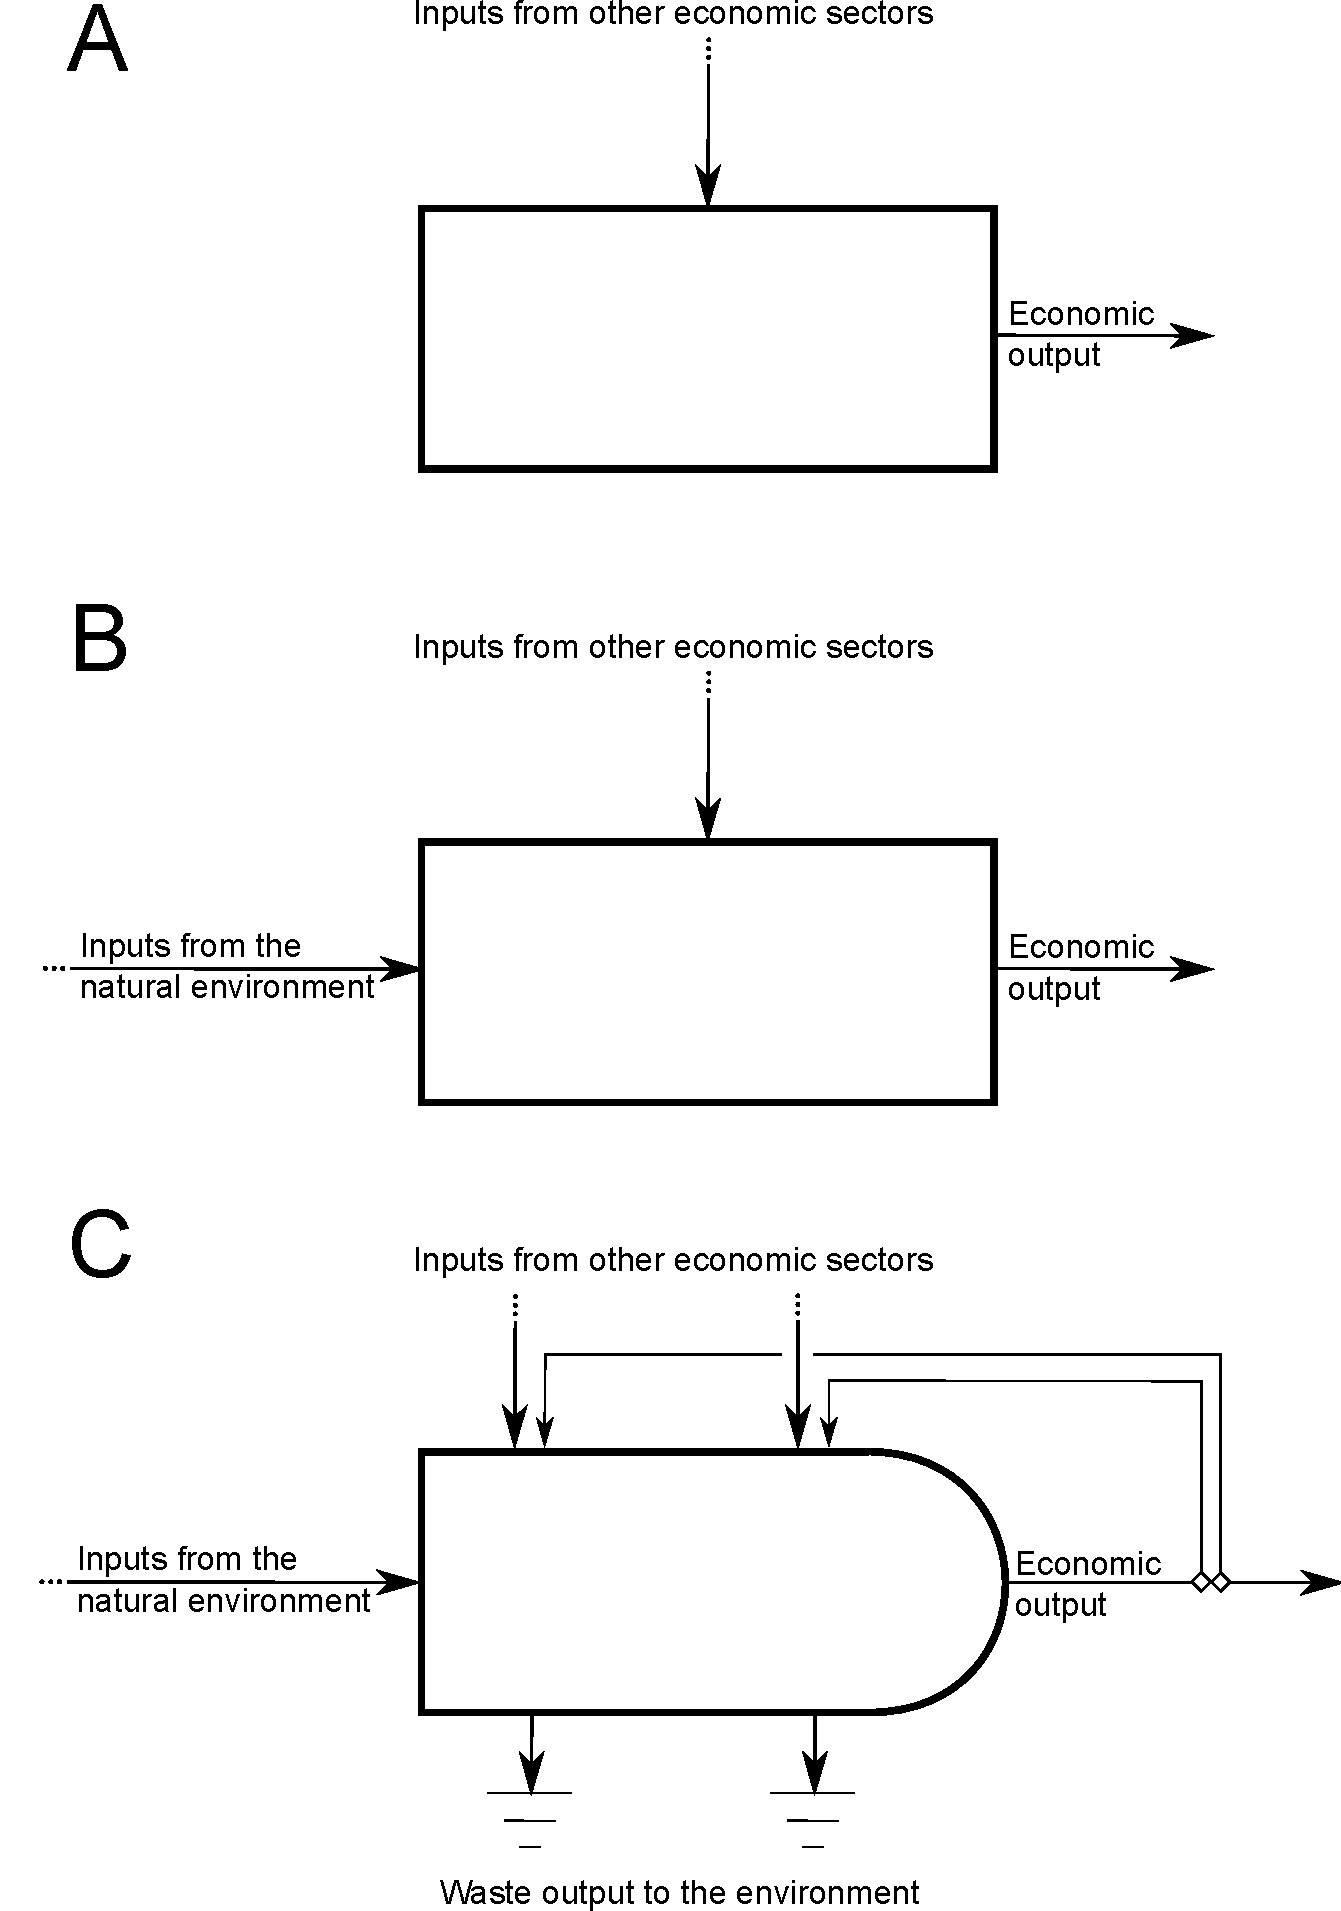
\includegraphics[width=0.8\linewidth]{images/Basic_unit_v3.pdf}
\caption{The basic unit of input-output modeling: A) the standard economic approach includes only transactions among sectors of the economy; B) the ecological economics approach models inputs from the natural environment outside the economy as factors of production and; C) the method presented here accounts also for accumulation, K, of embodied energy within materials in economic sectors.}
\label{fig:basic_unit}
\end{figure}

%%%%%%%%%% Methodology %%%%%%%%%%
\subsection{Total energy ($T$)}
%%%%%%%%%%

Total energy ($T$) is the sum of the direct and indirect (embodied) energy.

\begin{equation} \label{eq:T_def}
	T \equiv E + B
\end{equation}

In general, the flow rate of total energy among sectors in the economy, the earth, and society is given by

\begin{equation} \label{eq:T_dot_def}
	\dot{T} = \dot{E} + \dot{B}.
\end{equation}

In some cases, total energy flows may consist of direct energy ($\dot{E}$) or embodied energy ($\dot{B}$) exclusively. For example, the flow of extracted crude oil from the earth consists of direct energy only ($\dot{B} = 0$ and $\dot{T} = \dot{E}$), because, in this method, no embodied energy ($B$) has been added to the crude oil until it reaches the downstream side of the pump. The flow of goods produced by a non-energy sector of the economy consists of indirect energy only ($\dot{E} = 0$, and therefore $\dot{T} = \dot{B}$), because no direct energy ($E$) is produced by a non-energy sector in this model economy. 

In other cases, total energy flows may have both direct \emph{and} indirect components. For example, the flow of refined petroleum from the energy sector has both a direct energy ($\dot{E}$, the energy content of the oil product, usually represented by chemical potential energy) and embodied energy ($\dot{B}$, which accounts for the energy consumed in upstream processes to extract and refine the crude oil).\footnote{Outputs from agricultural sectors will be similar: both the direct energy component (comprising chemical potential energy) and the embodied energy component will be non-zero.}

Single subscripts on $T$, $E$, or $B$ can mean one of two things: $\dot{T}_{i}$ indicates the outflow of total energy from sector $i$, whereas $T_{i}$ denotes the total energy content of sector $i$. Double subscripts on $T$, $E$, or $B$ (e.g., $\dot{T}_{ij}$) indicate a flow from sector $i$ to sector $j$,\footnote{In the following discussion, the first index always indicates the sector \emph{from} which a quantity flows, and the second index indicates the sector \emph{to} which a quantity flows.} in this case for total energy ($T$).  

The I-O literature \cite{Bullard1975, Herendeen1978} [REF TO BULLARD AND HERENDEEN, ETC. HERE --MKH] assumes (a) that steady state conditions exist (i.e., no accumulation of total energy in economic sectors) and (b) that flows of total energy ($\dot{T}$) are \emph{conserved}, where by \emph{conserved}, it is meant that total energy can be neither created nor destroyed. Like the literature, we assume that total energy is conserved. However, we depart from the literature to allow durability of goods as represented by total energy accumulation in economic sectors. Steady state, this approach is not.

Total energy may accumulate within an economic sector as stocks of direct energy materials (piles of coal or tanks of oil) but also as embodied energy in stocks of capital goods (e.g. machinery or buildings). The rate of accumulation of total energy ($\frac{dT}{dt}$) in a sector of the economy, the Earth, or society is given by the time derivative of total energy:

\begin{equation} \label{eq:T_accum_def}
	\frac{\mathrm{d}T}{\mathrm{d}t} = \frac{\mathrm{d}E}{\mathrm{d}t} + \frac{\mathrm{d}B}{\mathrm{d}t}.
\end{equation}

We note that the definition of total energy (Equation \ref{eq:T_def}) includes direct energy ($E$) and embodied energy ($B$) terms. On the other hand, the First Law of Thermodynamics includes direct energy ($E$) and waste heat ($Q$) terms. The consequence of the foregoing difference is that an interesting relationship exists between embodied energy ($B$) and waste heat ($Q$). We shall see in the following example that waste heat from an economic sector can be considered to contribute to energy embodied within the products of that sector.

%%%%%%%%%%
\section{Example A: single sector economy}
%%%%%%%%%%

In this section, we present an example economic analysis using a single-sector economy wherein the economy and society are merged together.

Figure \ref{fig:single_sector_flows_0} shows a single-sector Economy (represented by ``economy/society,'' 2) that extracts direct energy from the earth ($\dot{E}_{12}$). Direct energy and waste heat flows are identified by vectors. No direct energy flows from the economy (2) to the earth (1), only waste heat ($\dot{Q}_{21}$).

\begin{figure}[h!]
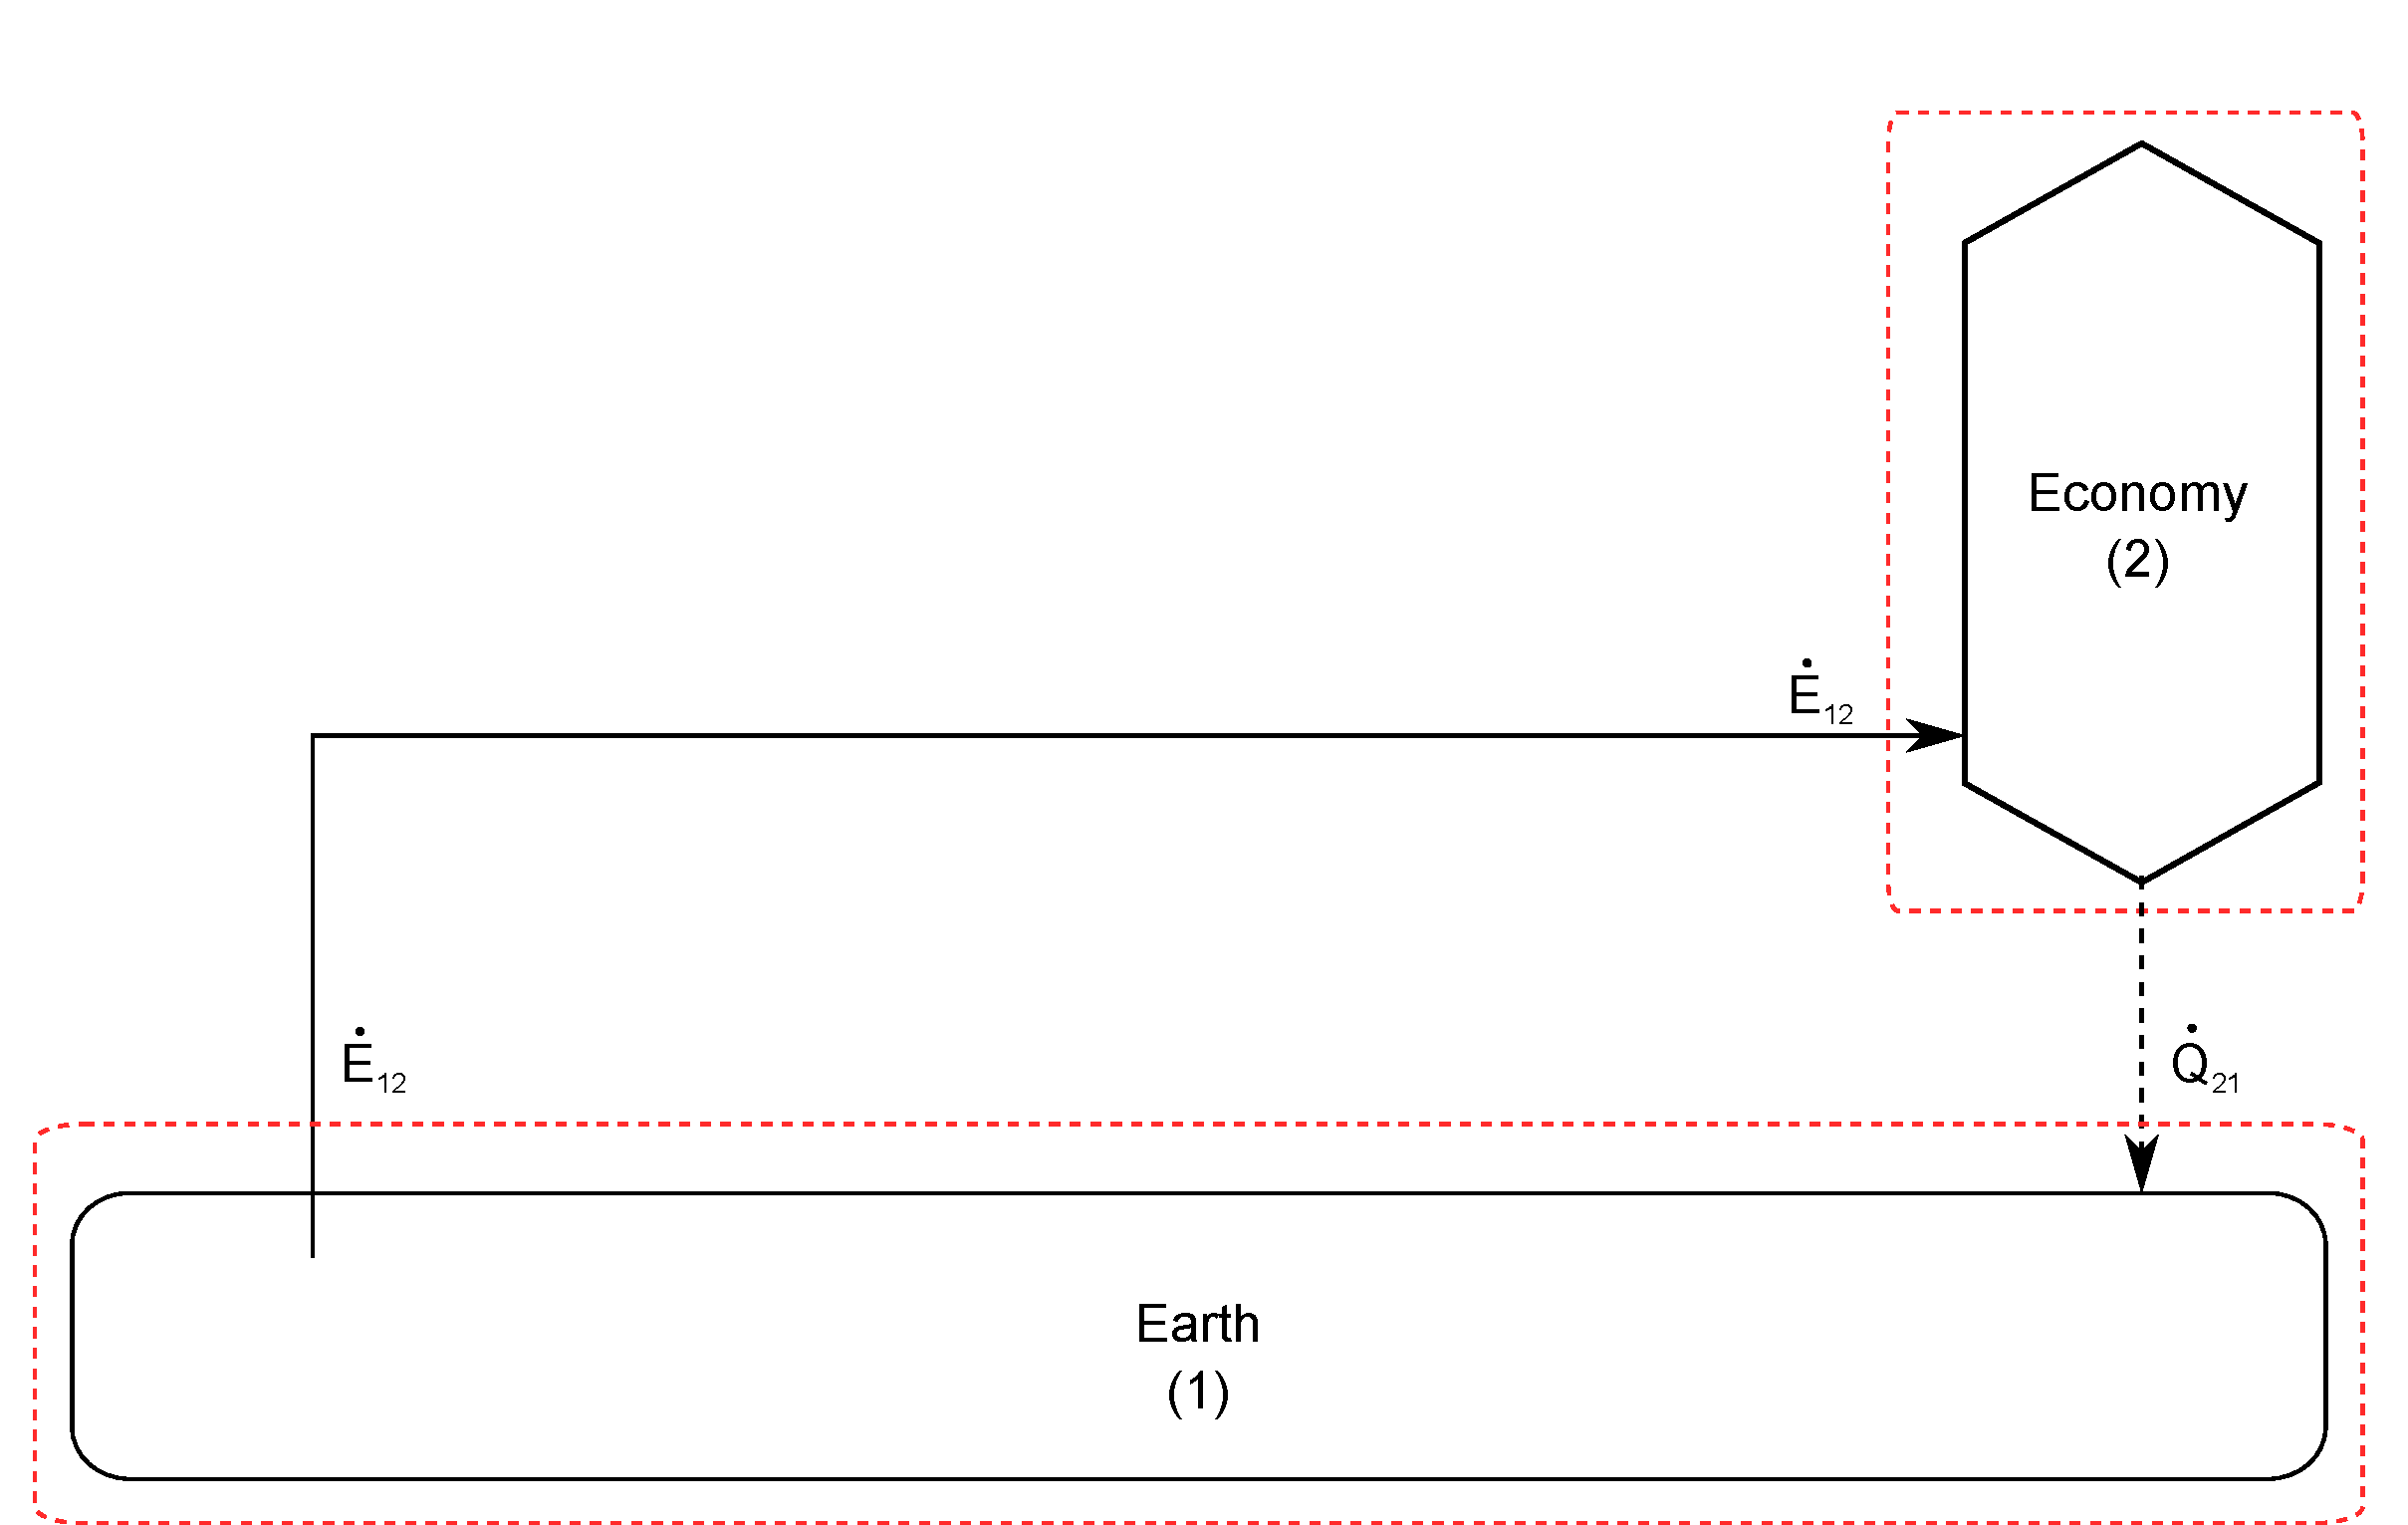
\includegraphics[width=1.0\linewidth]{images/I-O_one_sector_direct_energy.pdf}
\caption{Direct energy ($\dot{E}$) and waste heat ($\dot{Q}$) flows for a single-sector economy. }
\label{fig:single_sector_flows_0}
\end{figure}

%%%%%%%%%% Example A %%%%%%%%%%
\subsection{First Law of Thermodynamics}
%%%%%%%%%%

Both direct energy ($\dot{E}$, such as the energy content of coal, oil, and electricity), and waste heat ($\dot{Q}$) are accounted by the First Law of Thermodynamics. Accounting for possible accumulation of direct energy in the economy, the First Law of Thermodynamics indicates that

\begin{equation} \label{eq:dE_2/dt_single_sector}
	\frac{\mathrm{d}E_{2}}{\mathrm{d}t} = \dot{E}_{12} - \dot{Q}_{21}.
\end{equation}

Aside from, for example, the U.S. Strategic Petroleum Reserve, we are not stockpiling oil and coal at any meaningful rate, i.e. we consume fossil fuels at a rate equal to the extraction rate. Thus, the world is not accumulating direct energy in the economy.\footnote{A counter-example could be made for nuclear fuels where `spent' fuel represents a large exergetic stockpile, however, this reserve is not (presently) economically useful.} (The world \emph{is}, however, accumulating embodied energy in the economy as we shall see shortly.) Thus, the accumulation rate for direct energy $\left(\frac{\mathrm{d}E_{2}}{\mathrm{d}t}\right)$ in the above equation can be set to zero to obtain

\begin{equation} \label{eq:single_sector_direct_energy_no_accumulation}
	0 = \dot{E}_{12} - \dot{Q}_{21}.
\end{equation}

%%%%%%%%%% Example A %%%%%%%%%%
\subsection{Total energy accounting}
%%%%%%%%%%

Figure \ref{fig:single_sector_flows_2} shows the flows of total energy ($\dot{T}$) through the single-sector economy.

\begin{figure}[h!]
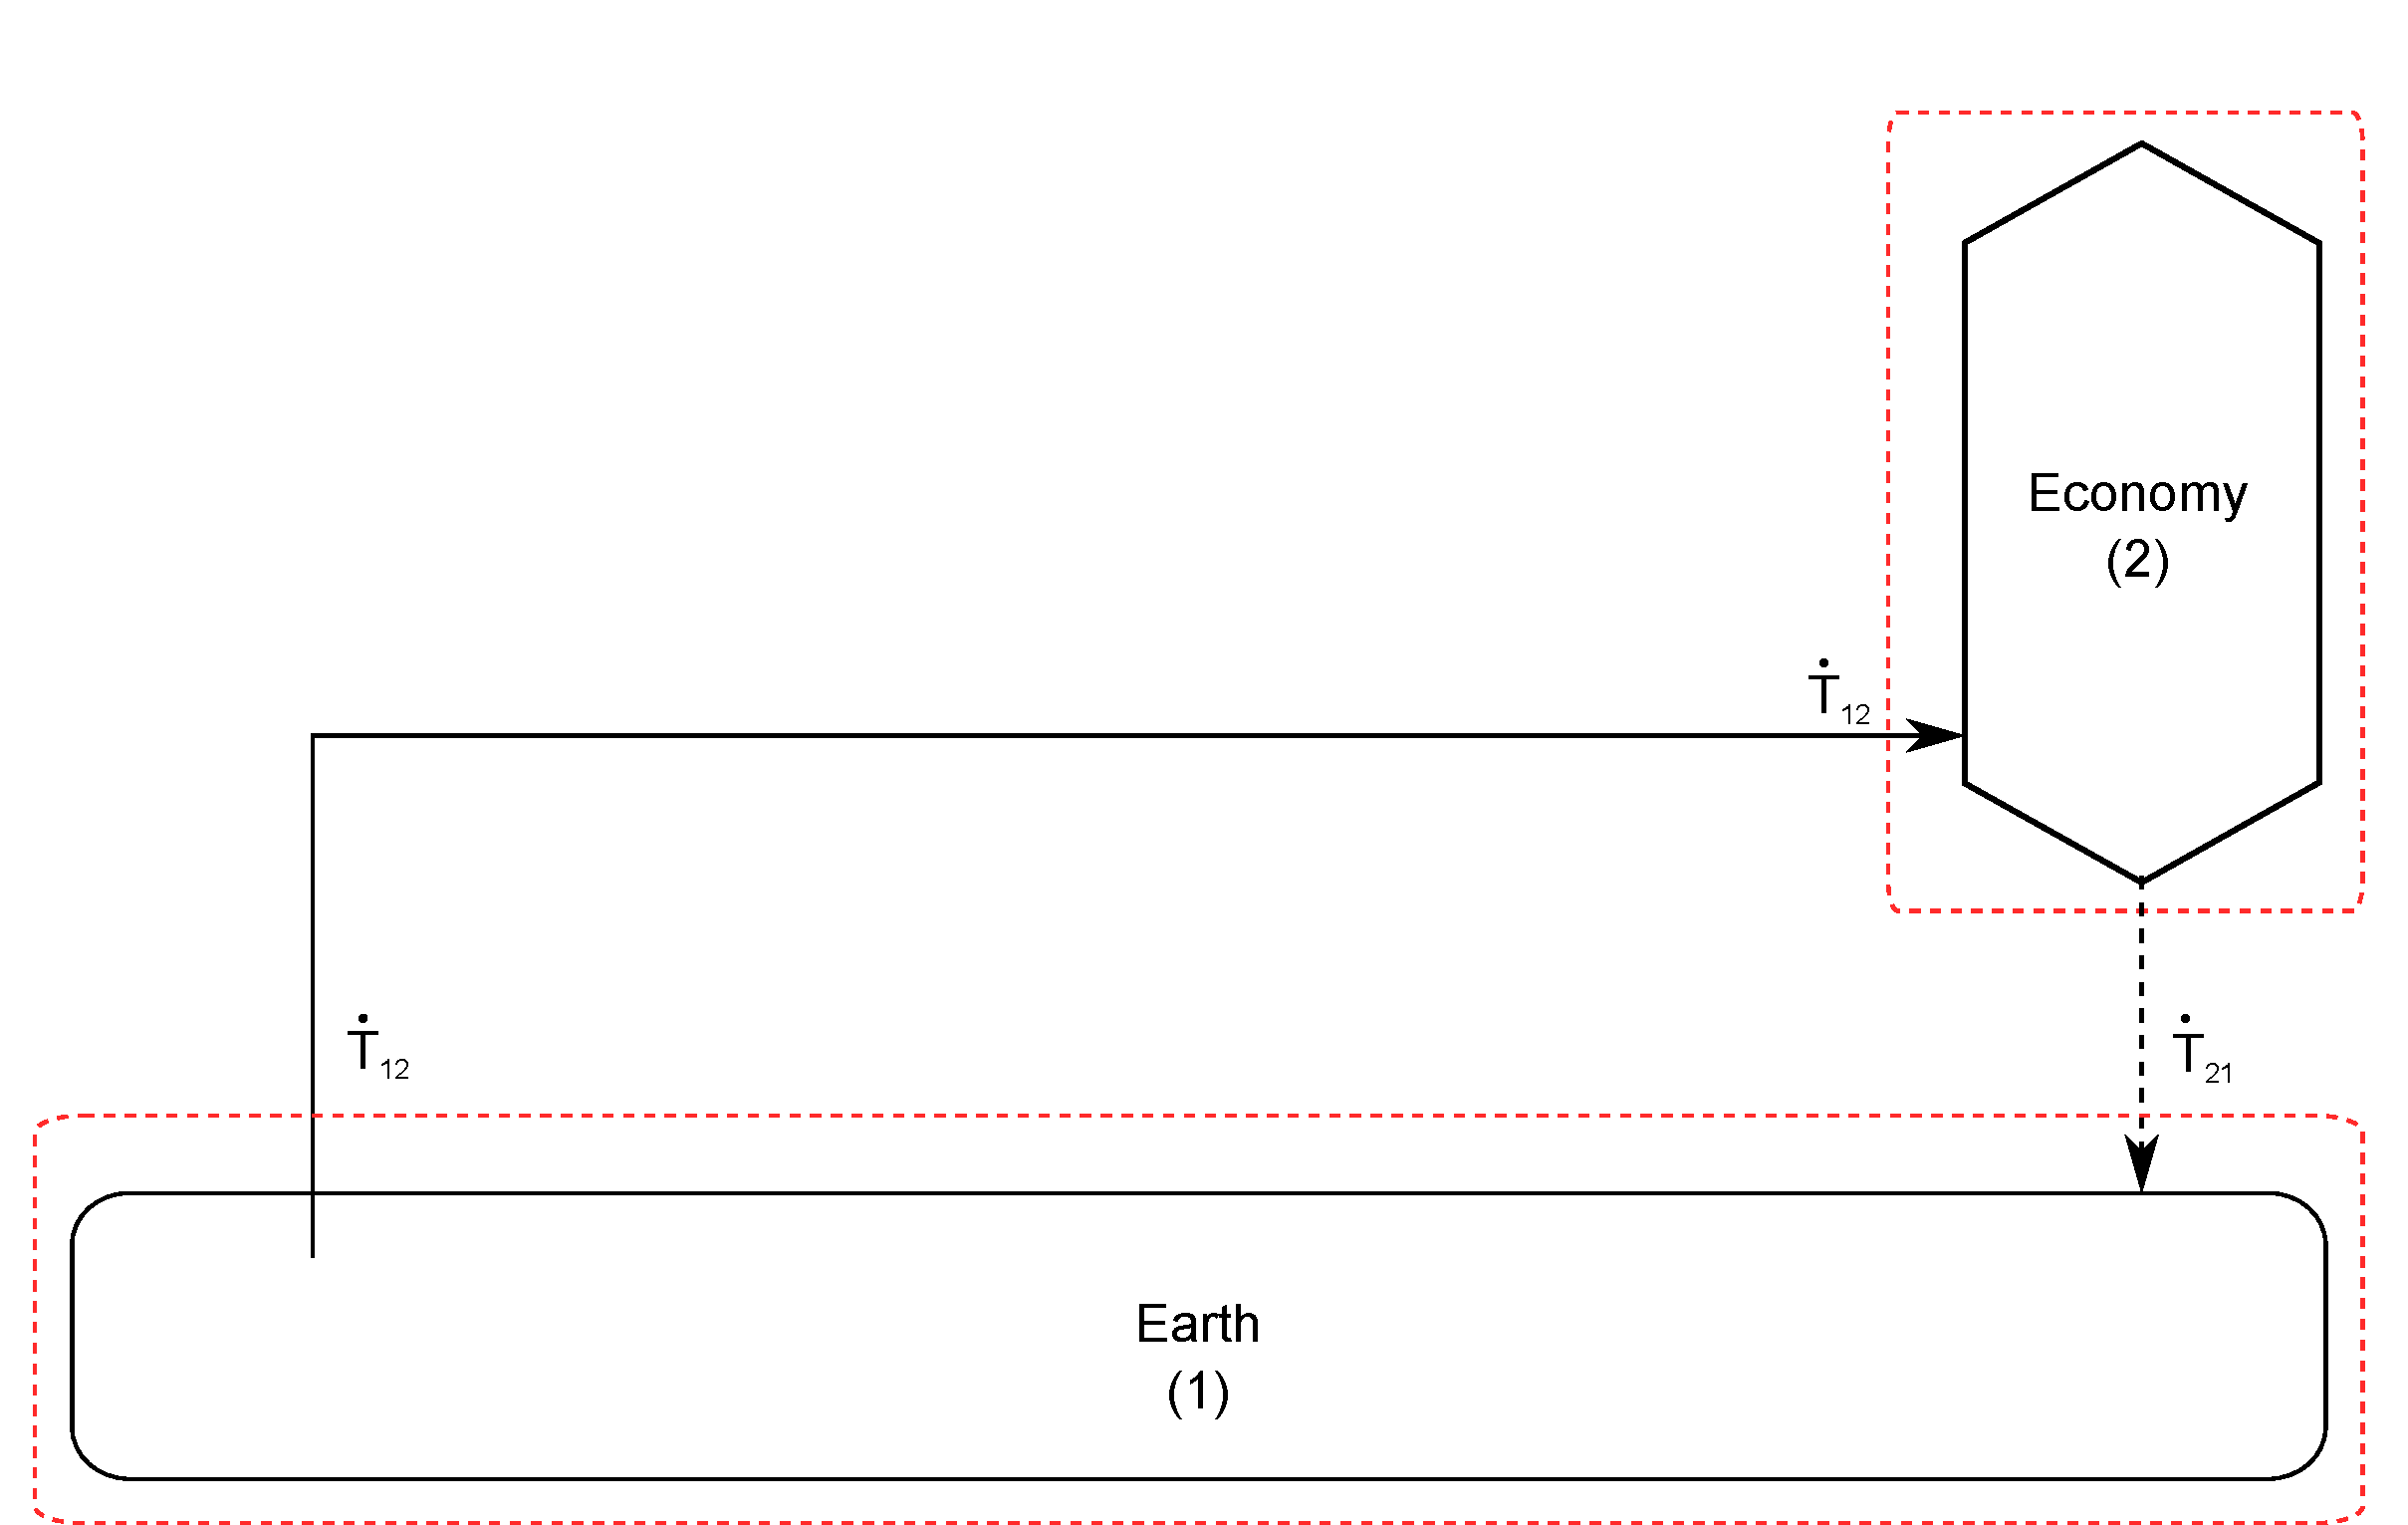
\includegraphics[width=1.0\linewidth]{images/I-O_one_sector_total_energy.pdf}
\caption{Total Energy Flows ($\dot{T}$) in a Single-sector Economy.}
\label{fig:single_sector_flows_2}
\end{figure}

We follow the I-O literature in assuming that total energy ($T$) is conserved. The I-O literature assumes steady-state operation of the economy with no accumulation of embodied energy in the economic sectors. (We will see later how the assumption in the literature introduces errors into I-O analyses.) We depart from the I-O literature by accounting for both accumulation and depreciation of energy embodied in sectors of the economy and society. By doing so, the present analysis does \emph{not} assume a steady-state economy. A total energy accounting around the single-sector economy (2) gives

\begin{equation} \label{eq:single_sector_T_with_accumulation}
	\frac{\mathrm{d}T_{2}}{\mathrm{d}t} = \dot{T}_{12}  - \dot{T}_{21}.
\end{equation}

%%%%%%%%%% Example A %%%%%%%%%%
\subsection{Embodied energy accounting}
%%%%%%%%%%

The First Law of Thermodynamics accounts for both direct energy ($E$) and waste heat ($Q$), whereas total energy ($T$) accounting tracks direct energy ($E$) and embodied energy ($B$). If we substitute the First Law into the total energy accounting equation, we can eliminate direct energy ($E$) to arrive at an embodied energy accounting equation. We begin by expanding the $T$ terms in Equation \ref{eq:single_sector_T_with_accumulation} using Equations \ref{eq:T_def} and \ref{eq:T_dot_def} to obtain

\begin{equation} \label{eq:single_sector_T_with_accumulation_expanded_T}
	\frac{\mathrm{d}E_{2}}{\mathrm{d}t} + \frac{\mathrm{d}B_{2}}{\mathrm{d}t} = \dot{E}_{12} + \dot{B}_{12} - \dot{E}_{21} - \dot{B}_{21}.
\end{equation}

\noindent Realizing that $\frac{\mathrm{d}E_2}{\mathrm{d}t} = 0$ (because direct energy does not accumulate in meaningful amounts in the economy) and $\dot{E}_{21} = 0$ (because energy is returned to the earth as waste heat, see Figure \ref{fig:single_sector_flows_0}) yields

\begin{equation} \label{eq:single_sector_B_accumulation}
	\frac{\mathrm{d}B_{2}}{\mathrm{d}t} = \dot{E}_{12} + \dot{B}_{12} - \dot{B}_{21}.
\end{equation}

\noindent Equation \ref{eq:single_sector_B_accumulation} shows that the accumulation rate of embodied energy in the economy is a function of the inflows of direct and embodied energy less the outflow of embodied energy. 

In this example, we substitute\footnote{We shall encounter this move to substitute the First Law of Thermodynamics into the total energy accounting equation repeatedly below.} Equation \ref{eq:single_sector_direct_energy_no_accumulation} into Equation \ref{eq:single_sector_B_accumulation} to obtain an embodied energy accounting equation:

\begin{equation} \label{eq:embodied_energy_accounting}
	\frac{\mathrm{d}B_{2}}{\mathrm{d}t} = \dot{Q}_{21} + \dot{B}_{12} - \dot{B}_{21}.
\end{equation}

An important result of Bullard-Herendeen-style I-O analyses, historically, has been the quantification of the embodied energy content of economic sector outputs, in this case $\dot{B}_{21}$. Equation \ref{eq:single_sector_B_accumulation} can be rearranged to give

\begin{equation} \label{eq:single_sector_B_output}
	\dot{B}_{21} = \dot{Q}_{21} + \dot{B}_{12} - \frac{\mathrm{d}B_{2}}{\mathrm{d}t}.
\end{equation}

Equation \ref{eq:single_sector_B_output} indicates that the embodied energy content of the product of an economic sector (in this case $\dot{B}_{21}$) can be thought of as the sum of the embodied energy inputs to the sector (in this case $\dot{B}_{12}$) and the waste heat from the sector (in this case $\dot{Q}_{21}$) less the accumulation rate of embodied energy in the sector (in this case $\frac{\mathrm{d}B_{2}}{\mathrm{d}t}$). This derivation indicates that waste heat ($\dot{Q}$) plays an important role\footnote{To our knowledge, there has been no prior identification of the role of waste heat in Bullard-Herendeen-style I-O analyses.} in Bullard-Herendeen-style I-O analyses: the accumulation of waste heat along a production path leads to energy being `embodied' in the output of an economic sector. 

In Equation \ref{eq:single_sector_B_output} we also see the first indication that the traditional approach of neglecting dynamic effects in I-O analyses may lead to errors. If $\frac{\mathrm{d}B_2}{\mathrm{d}t}$ is both neglected and nonzero, calculation of the embodied energy outflow rate ($\dot{B}_{21}$) will be in error.

%%%%%%%%%% Example A %%%%%%%%%%
\subsection{Depreciation}
%%%%%%%%%%

It is worthwhile to note that $\dot{B}_{21}$ represents the disposal rate of embodied energy from the economy back to the earth, akin to depreciation of physical assets. This physical depreciation is different from, but related to, financial depreciation, as financial depreciation is usually faster than physical depreciation. Embodied energy depreciation ($\dot{B}_{21}$ in this example) can be represented by a depreciation term such as

\begin{equation} \label{eq:depreciation_term_defined}
	\dot{B}_{21} = \gamma_{2}B_{2},
\end{equation}

\noindent where $\gamma$ represents the depreciation rate in units of inverse time (e.g., 1/year) with $\gamma > 0$. The depreciation rate ($\gamma$) indicates that a fraction of the total stock of embodied energy is disposed over a period of time (e.g, $\gamma = 0.05$/year). In the absence of other inputs or outputs, this depreciation function provides exponential decay of embodied energy ($B$). $\gamma$ is, in general, a function of time.

Equation \ref{eq:depreciation_term_defined} can be substituted into Equation \ref{eq:embodied_energy_accounting} and rearranged to obtain 

\begin{equation} \label{eq:dB2/dt_single_sector_with_depreciation_gamma}
	\frac{\mathrm{d}B_{2}}{\mathrm{d}t} =  \dot{Q}_{21} + \dot{B}_{12} - \gamma_{2}B_{2}
\end{equation}

\noindent which indicates that the accumulation rate of embodied energy in an economic sector (in this case $\frac{\mathrm{d}B_{2}}{\mathrm{d}t}$) is equal to the sum of the waste heat rate from the economic sector ($\dot{Q}_{21}$) and the inflow rate of embodied energy to the sector ($\dot{B}_{12}$) less the embodied energy disposal rate ($\gamma_{2}B_{2}$).


%%%%%%%%%%
\section{Value ($X$), energy intensity ($\varepsilon$), and the input-output ratio ($a$)}
%%%%%%%%%%

We now turn to defining flows of value ($\dot{X}$), energy intensity ($\varepsilon$), and input-output ratios ($a$).

%%%%%%%%%% X, epsilon, a %%%%%%%%%%
\subsection{Value flows ($\dot{X}$)}
%%%%%%%%%%

Among sectors of the economy and society, value ($\dot{X}$) flows in the same direction as goods, services, and energy, but in the opposite direction from currency payments. Typical of the Bullard-Herendeen I-O analyses technique [NEED REFERENCE HERE --MKH], we allow value flows to be in either monetary units or physical units. For non-energy sectors of the economy, value outflows are in currency units per time (\$/time). For energy-producing sectors, value outflows are in units of J/time or BTU/time.

%%%%%%%%%% X, epsilon, a %%%%%%%%%%
\subsection{Energy intensity ($\varepsilon$)}
%%%%%%%%%%

Energy intensity ($\varepsilon$) is the ratio of total energy and value outflow rates from an economic sector, such that for the $j^{\mathrm{th}}$ economic sector,

\begin{equation} \label{eq:epsilon_output_def}
	\varepsilon_{j} \equiv \frac{\dot{T}_{j}}{\dot{X}_{j}}.
\end{equation}

For goods and services sectors of the economy, $\varepsilon$ is in units of J/\$, but for energy-producing sectors of the economy, the units of $\varepsilon$ are J/J. For inter-sector flows, we have

\begin{equation} \label{eq:epsilon_transfers_1}
	\varepsilon_{ij} = \frac{\dot{T}_{ij}}{\dot{X}_{ij}}.
\end{equation}

\noindent Furthermore, we note that 

\begin{equation} \label{eq:epsilon_equiv_1}
	\varepsilon_{i} = \varepsilon_{ij}
\end{equation}

\noindent for all $j$, because the energy intensity of a sector's output is the same regardless of its destination. I.e., we assume that all goods produced within a sector are produced at the average energy intensity of that sector.\footnote{If this approach is unsatisfactory, the sector may be divided into sub-sectors with different energy intensities.}

%%%%%%%%%% X, epsilon, a %%%%%%%%%%
\subsection{Input-output ratios ($a$)}
%%%%%%%%%%

We define a parameter $a_{ij}$ that represents the input of good $i$ required to produce a unit of output from sector $j$.

\begin{equation} \label{eq:aij_def}
	a_{ij} \equiv \frac{\dot{X}_{ij}}{\dot{X}_{j}}
\end{equation}

Input-output ratios are given in mixed units, depending on the purpose of each sector of the economy and the type of input as shown in Table \ref{table: A_matrix_units}.

\begin{table}
\caption{Units for input-output ratios ($a$).}
\begin{center}
  \begin{tabular}{ ll | c  c | }
 			& 							& \multicolumn{2}{|c|}{Output of} \\
    		&	 						& Non-energy sector 		& Energy sector \\ \hline
\multirow{2}{*}{Inputs from}    		& Non-energy sector 	& $\frac{\text{\$}}{\text{\$}}$ 	& $\frac{\text{\$}}{\text{J}}$ \\ 
    		& Energy sector	 	& $\frac{\text{J}}{\text{\$}}$ 	& $\frac{\text{J}}{\text{J}}$ \\ \hline
  \end{tabular}
\end{center}
\label{table: A_matrix_units}
\end{table}

%%%%%%%%%%
\section{Example B: a one sector economy with external demand}
%%%%%%%%%%

At this point, we move to a second example wherein a single economic sector (3) interacts with Society (2, which provides final demand) and the Earth (1, the destination for waste heat and the source of all resources). In this economy, we assume that the purpose of the goods and services sector is to produce goods and provide services, including the provision of direct energy available to the economy and society.

%%%%%%%%%% Example B %%%%%%%%%%
\subsection{First Law of Thermodynamics}
%%%%%%%%%%

The First Law of Thermodynamics requires that energy (direct and wast heat) is conserved around each Sector of the economy (3) as well as around the Earth (1) and Society (2) as shown in Figure \ref{fig:direct_energy_flows}. 

\begin{figure}[h!]
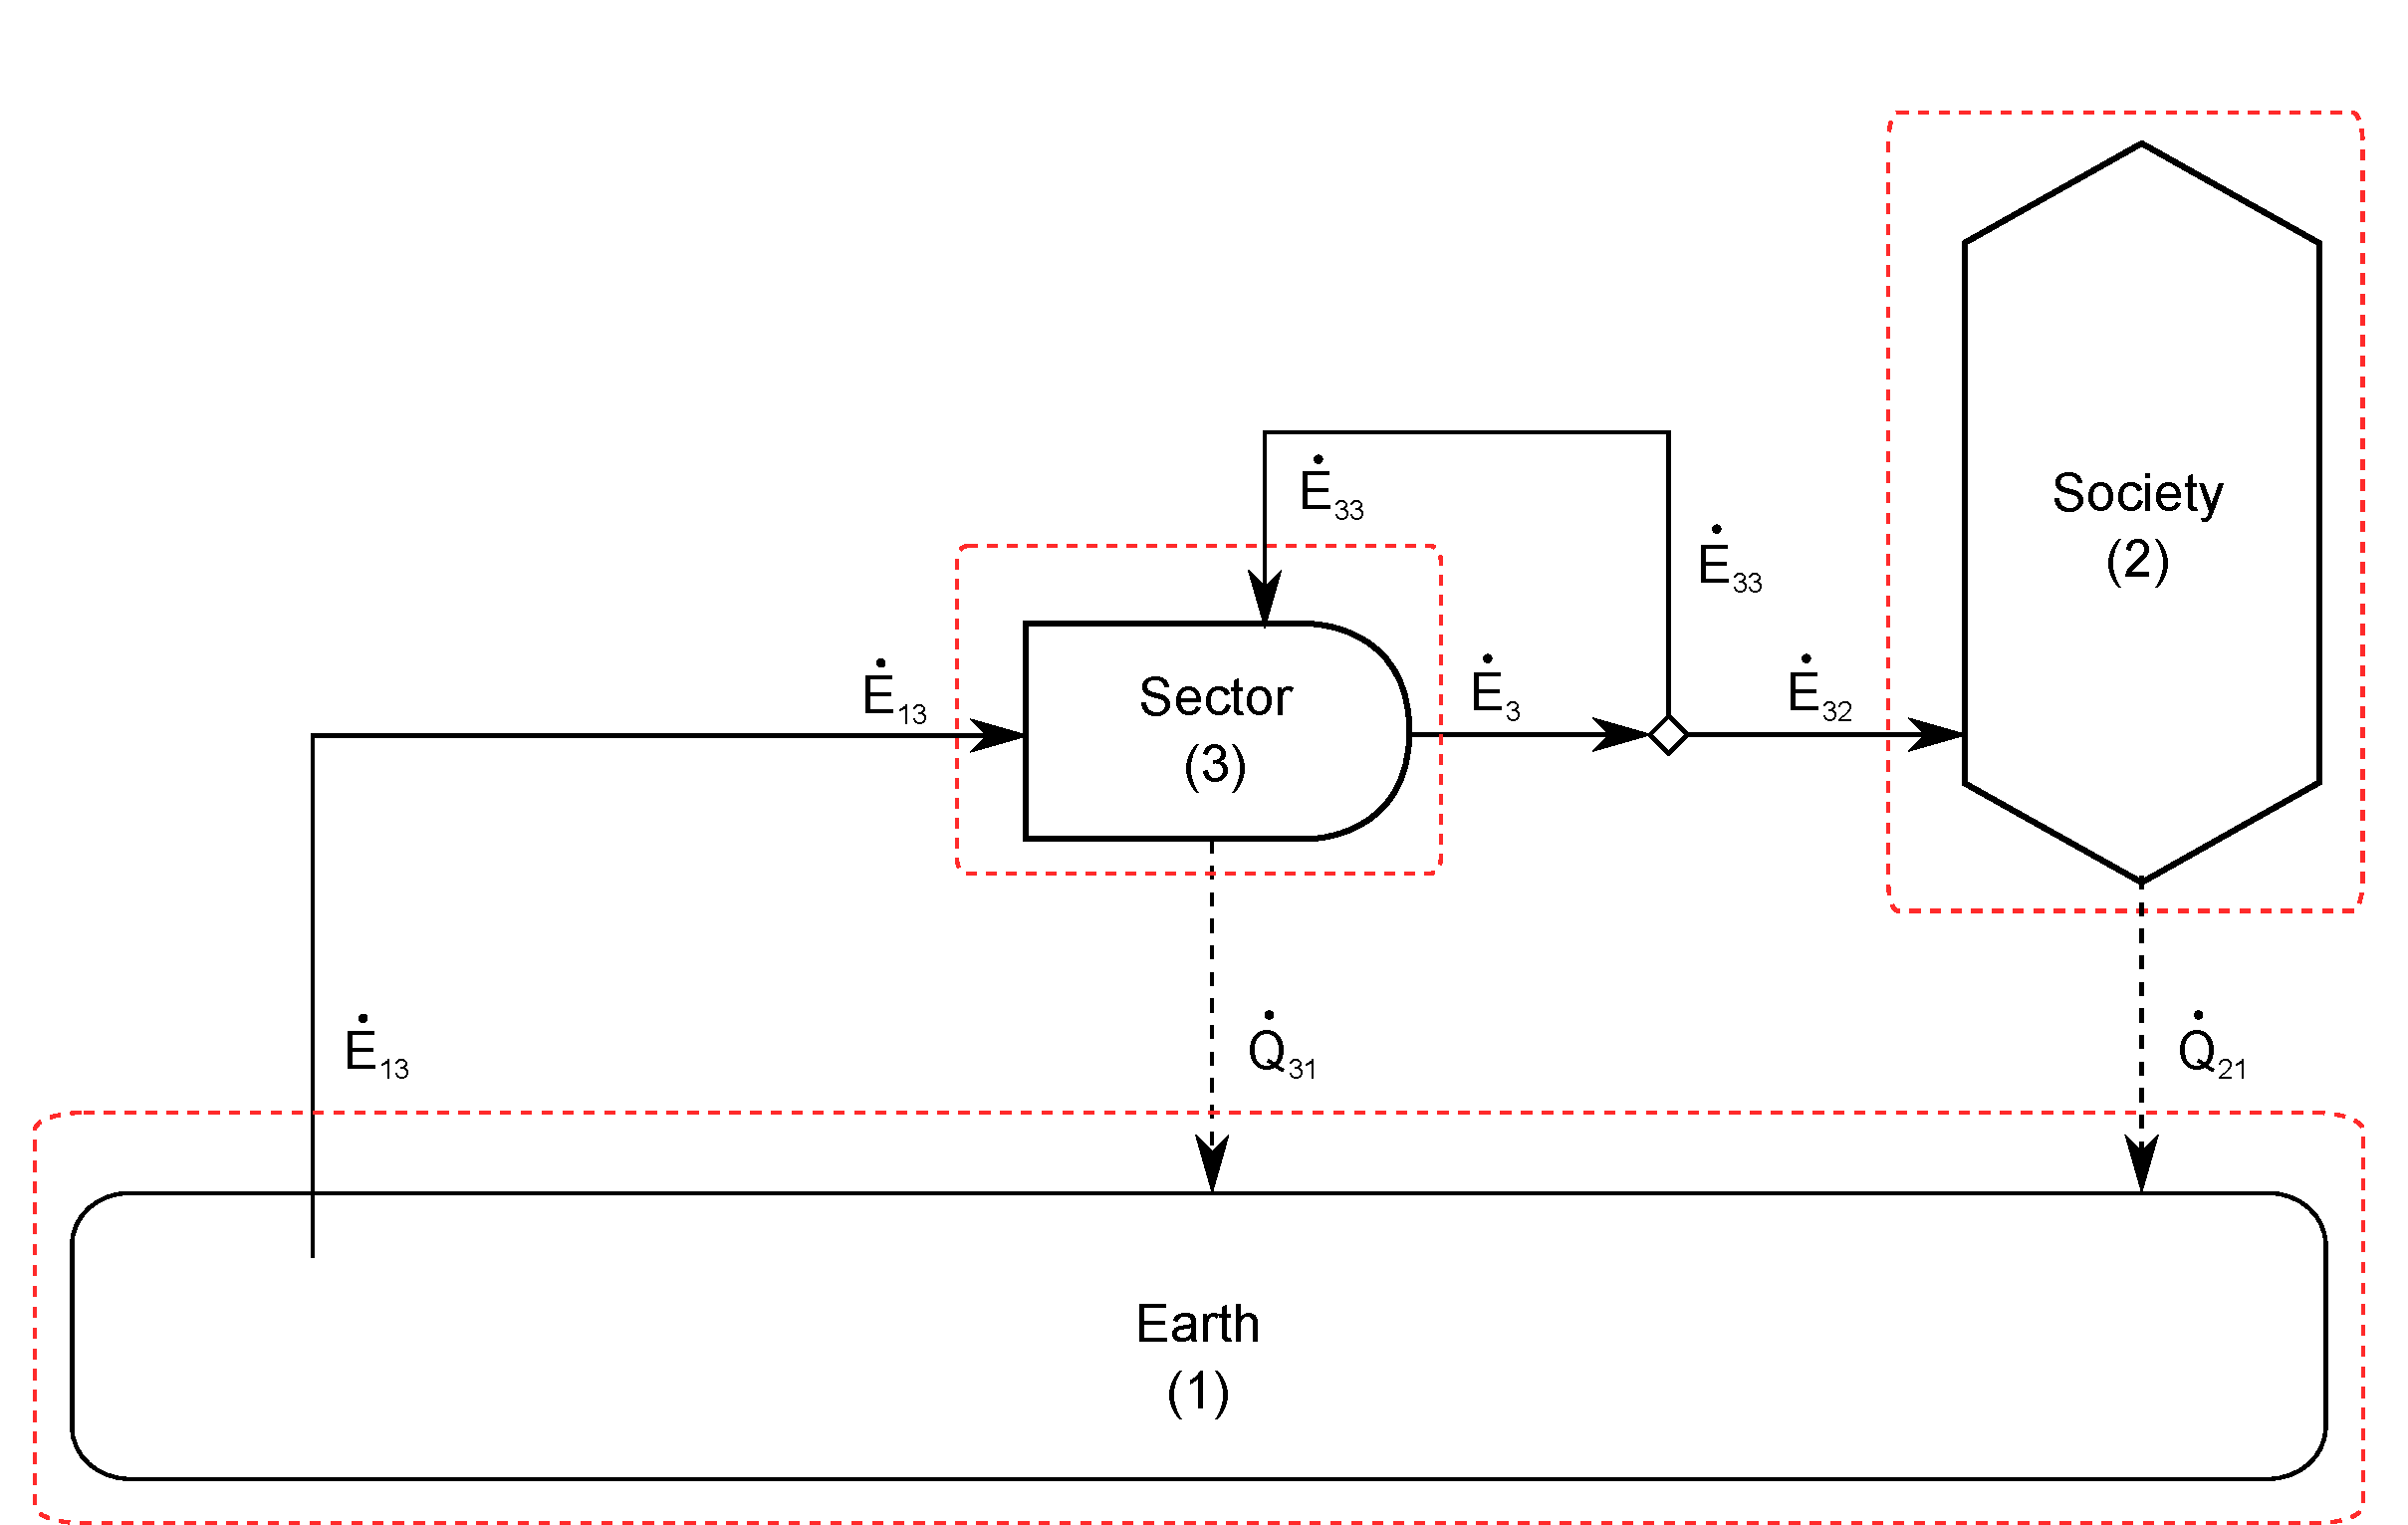
\includegraphics[width=1.0\linewidth]{images/I-O_two_sector_direct_energy.pdf}
\caption{Flows of direct energy ($\dot{E}$) and waste heat ($\dot{Q}$) in a one-sector economy with separate demand.}
\label{fig:direct_energy_flows}
\end{figure}

The First Law around the economic Sector (3) including the accumulation rate of direct energy in the sector $\left(\frac{\mathrm{d}E_{3}}{\mathrm{d}t}\right)$ yields

\begin{equation} \label{eq:CV_E_dot_3}
	\frac{\mathrm{d}E_{3}}{\mathrm{d}t} 	 = \dot{E}_{13} + \dot{E}_{33} - \dot{E}_{3} - \dot{Q}_{31}.
\end{equation}

\noindent It is notable that the economic Sector (3) consumes a portion of its own energy output ($\dot{E}_{33}$) as it produces its goods and services: it takes energy to make energy.

First Law energy accounting around the Earth (1) and Society (2) gives

\begin{equation} \label{eq:CV_E_dot_1}
	\frac{\mathrm{d}E_{1}}{\mathrm{d}t} 	 =  \dot{Q}_{21} + \dot{Q}_{31} - \dot{E}_{13},
\end{equation}

\noindent and 

\begin{equation} \label{eq:CV_E_dot_2}
	\frac{\mathrm{d}E_{2}}{\mathrm{d}t} 	 = \dot{E}_{32} - \dot{Q}_{21}.
\end{equation}

As in Example A, we can set the accumulation of direct energy within each sector to zero to obtain

\begin{equation} \label{eq:CV_E_dot_3_SS}
	0 =\dot{E}_{13} + \dot{E}_{33} - \dot{E}_{3} - \dot{Q}_{31},
\end{equation}

\begin{equation} \label{eq:CV_E_dot_1_SS}
	0 =  \dot{Q}_{21} + \dot{Q}_{31} - \dot{E}_{13},
\end{equation}

\noindent and 

\begin{equation} \label{eq:CV_E_dot_2_SS}
	0 =\dot{E}_{32} - \dot{Q}_{21},
\end{equation}

%%%%%%%%%%% Example B %%%%%%%%%%
%\subsection{Energy ratios}
%%%%%%%%%%%
%
%[IS THERE ANY POINT IN DEFINING THESE HERE IF THEY ARE NOT USED? I HAVE COMMENTED THEM OUT AS I THINK THEY HAVE BEEN MOVED TO LATER SECTION IN EXAMPLE C - MD]
%
%Several important energy ratios can be observed in Figure \ref{fig:direct_energy_flows}. The Gross Energy Ratio ($GER$) is defined as 
%
%\begin{equation} \label{eq:GER_def_ch_5}
%	GER \equiv \frac{\dot{E}_{3}}{\dot{E}_{33}}.
%\end{equation}
%
%\noindent The Net Energy Ratio ($NER$) is defined as
%
%\begin{equation} \label{eq:NER_def_ch_5}
%	NER \equiv \frac{\dot{E}_{32}}{\dot{E}_{33}} = GER - 1.
%\end{equation}
%
%[THESE DEFINITIONS ARE EQUIVALENT TO $\beta$ BOUNDARY DEFINED IN BRANDT AND DALE (2011). WE CANNOT DISTINGUISH EXTERNAL ENERGY RATIOS AT THIS POINT. NOT SURE ABOUT COMMENTED WORK BELOW - CHECK TEX FILE.]

%The rate of energy extracted from the Earth can be expressed as either
%
%\begin{equation} \label{eq:E_dot_13_a}
%	\dot{E}_{13} = \frac{GER - 1}{NEER}\dot{E}_{22}
%\end{equation}
%
%\noindent or
%
%\begin{equation} \label{eq:E_dot_32_b}
%	\dot{E}_{32} = \frac{1 - \frac{1}{GER}}{NEER}\dot{E}_{2}.
%\end{equation}

%%%%%%%%%% Example B %%%%%%%%%%
\subsection{Total energy accounting}
%%%%%%%%%%

Again, we follow the I-O literature in assuming that total energy (i.e., the sum of direct energy and indirect energy) is conserved. Thus, we can draw a diagram similar to Figure \ref{fig:direct_energy_flows} for total energy flows. See Figure \ref{fig:total_energy_flows_1S}.

\begin{figure}[h!]
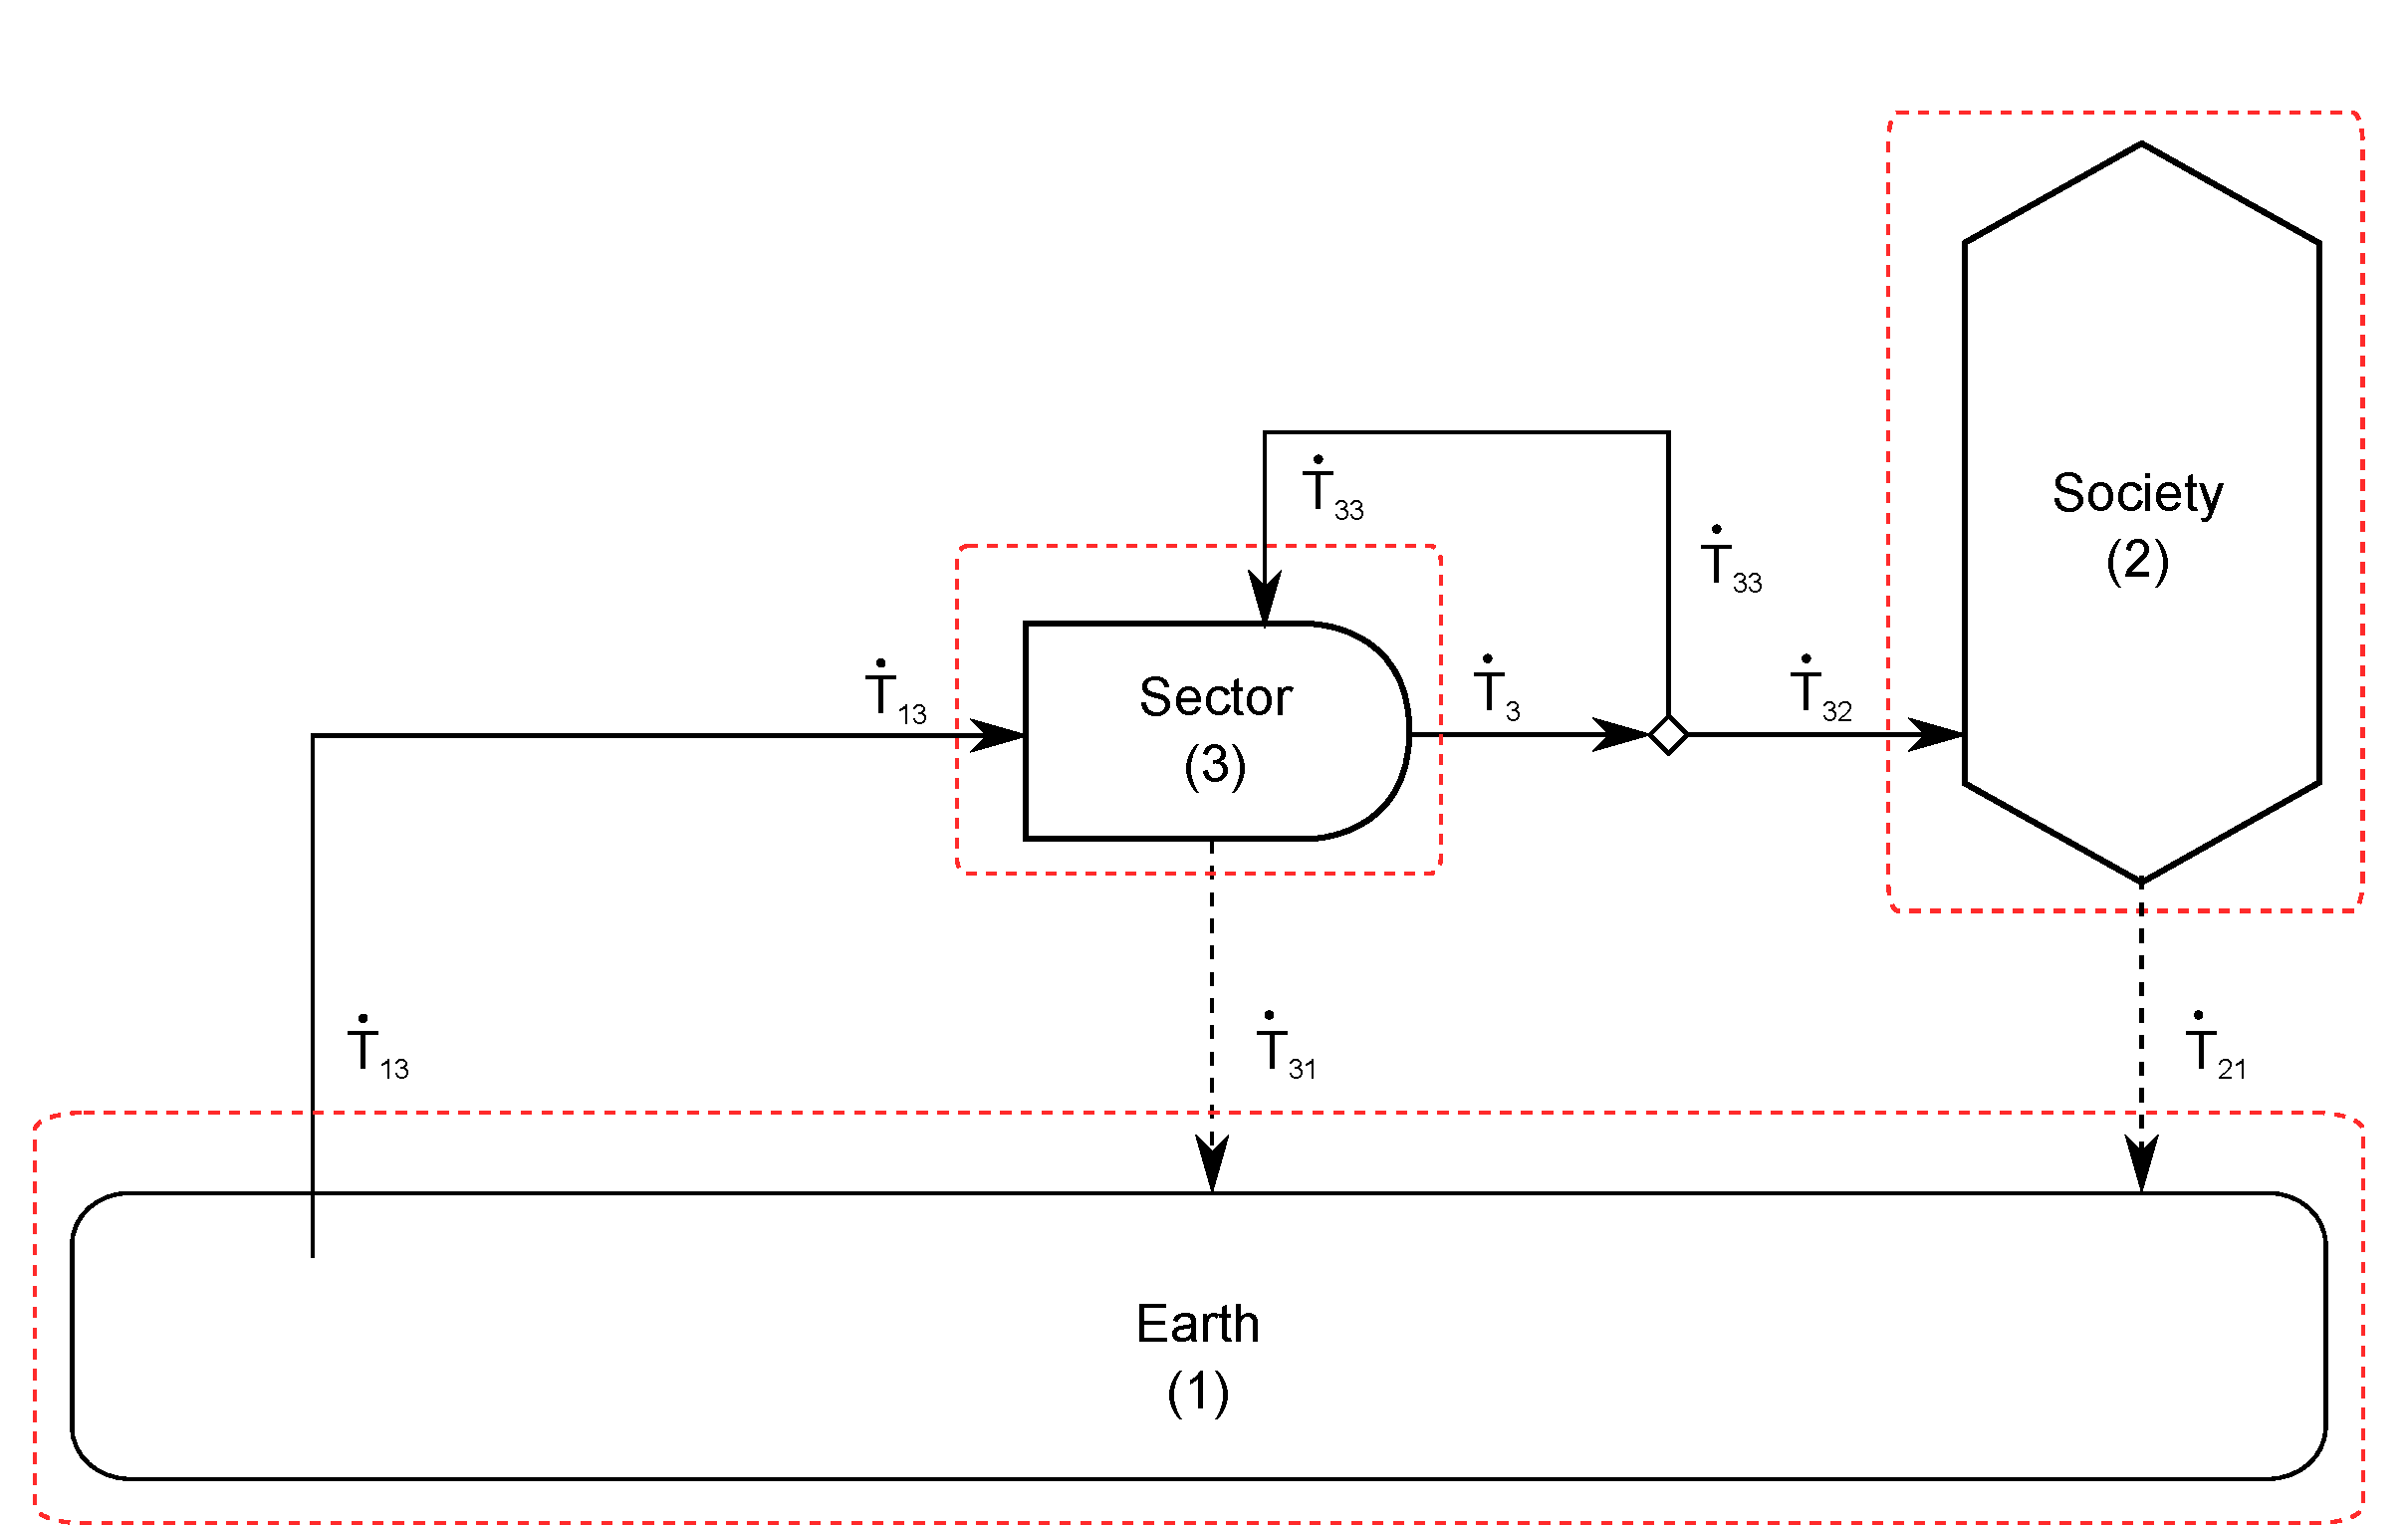
\includegraphics[width=1.0\linewidth]{images/I-O_two_sector_total_energy.pdf}
\caption{Flows of total energy ($\dot{T}$) in a one-sector economy with separate demand.}
\label{fig:total_energy_flows_1S}
\end{figure}

Accounting for accumulation of total energy and using the assumption that total energy is conserved, we can write the following equations.

\begin{equation} \label{eq:CV_T_1}
	\frac{\mathrm{d}T_{1}}{\mathrm{d}t} 	 = \dot{T}_{21} + \dot{T}_{31} - \dot{T}_{13},
\end{equation}

\begin{equation} \label{eq:CV_T_2}
	\frac{\mathrm{d}T_{2}}{\mathrm{d}t} 	 = \dot{T}_{32} - \dot{T}_{21},
\end{equation}

\noindent and

\begin{equation} \label{eq:CV_T_3}
	\frac{\mathrm{d}T_{3}}{\mathrm{d}t} 	 = \dot{T}_{13} + \dot{T}_{33} - \dot{T}_{3} - \dot{T}_{31}.
\end{equation}

%%%%%%%%%% Example B %%%%%%%%%%
\subsection{Embodied energy accounting}
%%%%%%%%%%

Given that $\frac{\mathrm{d}E_{i}}{\mathrm{d}t} = 0$ and $\dot{T} = \dot{E} + \dot{B}$, we note that

\begin{equation} \label{eq:T_dot_equals_B_dot}
	\frac{\mathrm{d}T_i}{\mathrm{d}t} = \frac{\mathrm{d}B_i}{\mathrm{d}t},
\end{equation}

\noindent and we can rewrite the total energy accumulation accounting equations as

\begin{equation} \label{eq:CV_dB_1}
	\frac{\mathrm{d}B_{1}}{\mathrm{d}t} = \dot{E}_{21} + \dot{B}_{21} + \dot{E}_{31} + \dot{B}_{31} - \dot{E}_{13} + \dot{B}_{13},
\end{equation}

\begin{equation} \label{eq:CV_dB_2}
	\frac{\mathrm{d}B_{2}}{\mathrm{d}t} = \dot{E}_{32} + \dot{B}_{32} - \dot{E}_{21} - \dot{B}_{21},
\end{equation}

\noindent and 

\begin{equation} \label{eq:CV_dB_3}
	\frac{\mathrm{d}B_{3}}{\mathrm{d}t} = \dot{E}_{13} + \dot{B}_{13} + \dot{E}_{33} + \dot{B}_{33} - \dot{E}_{3} - \dot{B}_{3} - \dot{E}_{31} - \dot{B}_{31}.
\end{equation}

As in Example A, we can substitute the First Law of Thermodynamics for the economic Sector (Equation \ref{eq:CV_E_dot_3_SS}) into the total energy accounting equation for the economic Sector (Equation \ref{eq:CV_dB_3}). Assuming that $\dot{E}_{31} = 0$ (because energy is returned to the Earth as waste heat, not direct energy), we obtain

\begin{equation} \label{eq:ExB_embodied_energy_accounting}
	\frac{\mathrm{d}B_3}{\mathrm{d}t} = \dot{Q}_{31} + \dot{B}_{13} + \dot{B}_{33} - \dot{B}_{31}
\end{equation}

Similar to Example A, we observe that the accumulation rate of embodied energy in the Goods and Services sector (3) is the sum of the rates of waste heat from the sector ($\dot{Q}_{31}$) and embodied energy into the sector ($\dot{B}_{13} + \dot{B}_{33}$) less the rate of embodied energy leaving the sector on its output stream ($\dot{B}_{31}$).

%%%%%%%%%% Example B %%%%%%%%%%
\subsection{Depreciation}
%%%%%%%%%%

We can substitute a depreciation term for the flow rate of embodied energy from the economic Sector (3) to the Earth (1) to obtain

\begin{equation} \label{eq:ExB_embodied_energy_accounting_with_depreciation}
	\frac{\mathrm{d}B_3}{\mathrm{d}t} = \dot{Q}_{31} + \dot{B}_{13} + \dot{B}_{33} - \gamma_3 B_3.
\end{equation}

%%%%%%%%%% Example B %%%%%%%%%%
\subsection{Estimating energy intensity ($\varepsilon$) of the economy}
%%%%%%%%%%

The following figure shows value flows ($\dot{X}$) in the one-sector economy with separate demand.

\begin{figure}[H]
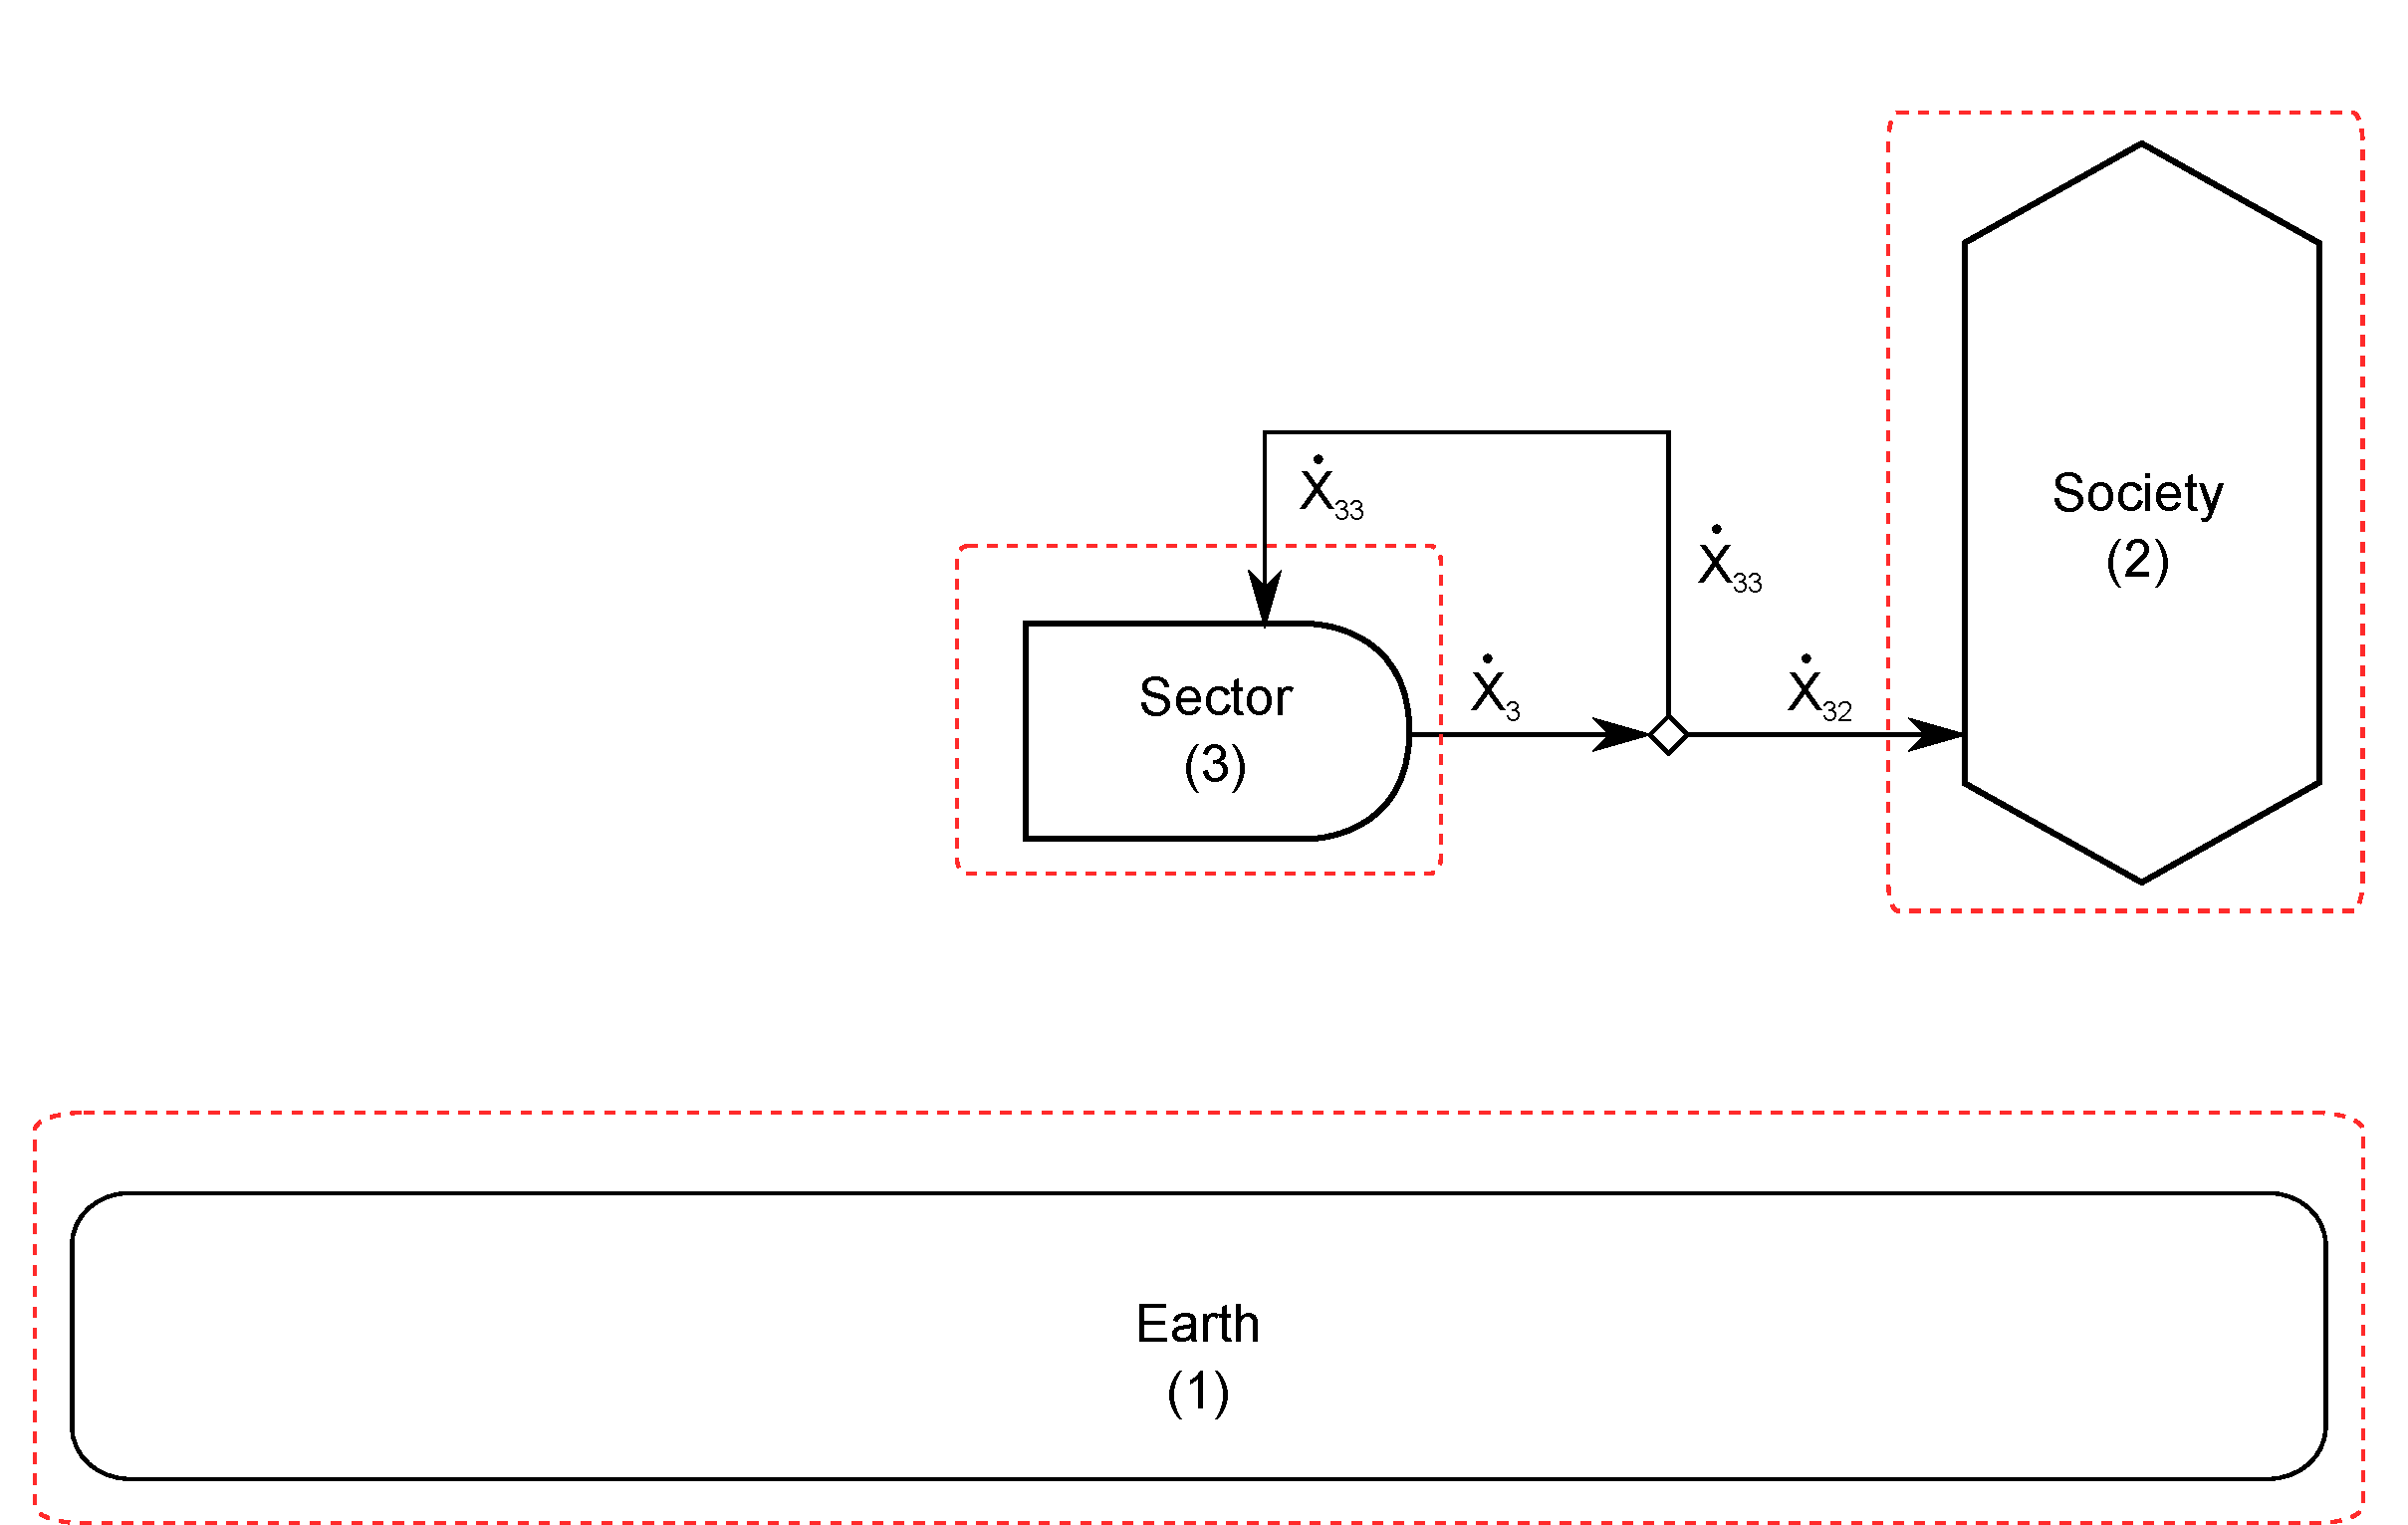
\includegraphics[width=1.0\linewidth]{images/I-O_two_sector_value.pdf}
\caption{Flows of economic value ($\dot{X}$) in a one-sector economy with separate demand.}
\label{fig:economic_value_flows}
\end{figure}

The energy intensity ($\varepsilon$) of the economic Sector (3) is given by

\begin{equation} \label{eq:single_sector_energy_intensity}
	\varepsilon_{3} = \frac{\dot{T}_{3}}{\dot{X}_{3}} = \frac{\dot{T}_{33}}{\dot{X}_{33}}.
\end{equation}

The input-output ratio ($a$) for the economic Sector (3) is

\begin{equation} \label{eq:io_ratio_single_sector}
	a_{33} = \frac{\dot{X}_{33}}{\dot{X}_{3}}.
\end{equation}

\noindent Thus,

\begin{equation} \label{eq:T_dot_1_single_sector}
	\dot{T}_{3} = \varepsilon_{3}\dot{X}_{3},
\end{equation}

\noindent and

\begin{equation} \label{eq:T_dot_11_single_sector}
	\dot{T}_{33} = \varepsilon_{3}a_{33}\dot{X}_{3}.
\end{equation}

Realizing that (a) $\frac{\mathrm{d}T_3}{\mathrm{d}t} = \frac{\mathrm{d}B_3}{\mathrm{d}t}$ because $\frac{\mathrm{d}E_3}{\mathrm{d}t} = 0$, (b) $\dot{T}_{13} = \dot{E}_{13}$ because $\dot{B}_{13} = 0$ due to processing of raw energy carriers occurring \emph{within} the economic Sector (3), and (c) substituting Equations \ref{eq:T_dot_1_single_sector} and \ref{eq:T_dot_11_single_sector} into Equation \ref{eq:CV_T_3} gives

\begin{equation} \label{eq:dB1/dt_single_sector_after_substituting_eps_and_a}
	\frac{\mathrm{d}B_{3}}{\mathrm{d}t} = \varepsilon_{3}a_{33}\dot{X}_{3} + \dot{E}_{13} - \varepsilon_{3}\dot{X}_{3} - \gamma_{3}B_{3}.
\end{equation}

We can estimate the energy intensity of the economy by solving Equation \ref{eq:dB1/dt_single_sector_after_substituting_eps_and_a} for $\varepsilon_{3}$.

\begin{equation} \label{eq:eps3_ss_IO}
	\varepsilon_{3} = (1 - a_{33})^{-1} \dot{X}_{3}^{-1} \left[\dot{E}_{13} - \left(\frac{\mathrm{d}B_{3}}{\mathrm{d}t} + \gamma_{3}B_{3}\right)\right]
\end{equation}

Equation \ref{eq:eps3_ss_IO} is similar to the typical energy intensity equation found in the I-O literature [REFERENCE BULLARD AND OTHERS HERE. --MKH], except that Equation \ref{eq:eps3_ss_IO} applies to a single economic sector and contains scalar (as opposed to matrix) terms. Using Example C below, we will derive a matrix representation of Equation \ref{eq:eps3_ss_IO} that is directly comparable to energy intensity equations found in the I-O literature.

%%%%%%%%% Example B %%%%%%%%%%
\subsection{Derivation of economic sector energy intensity ($\varepsilon$) by a convergent infinite series}
%%%%%%%%%%

The single-sector economy of Figures \ref{fig:direct_energy_flows} through \ref{fig:economic_value_flows} can be re-drawn as shown in Figure \ref{fig:single_sector_flows_3}.

\begin{figure}[h!]
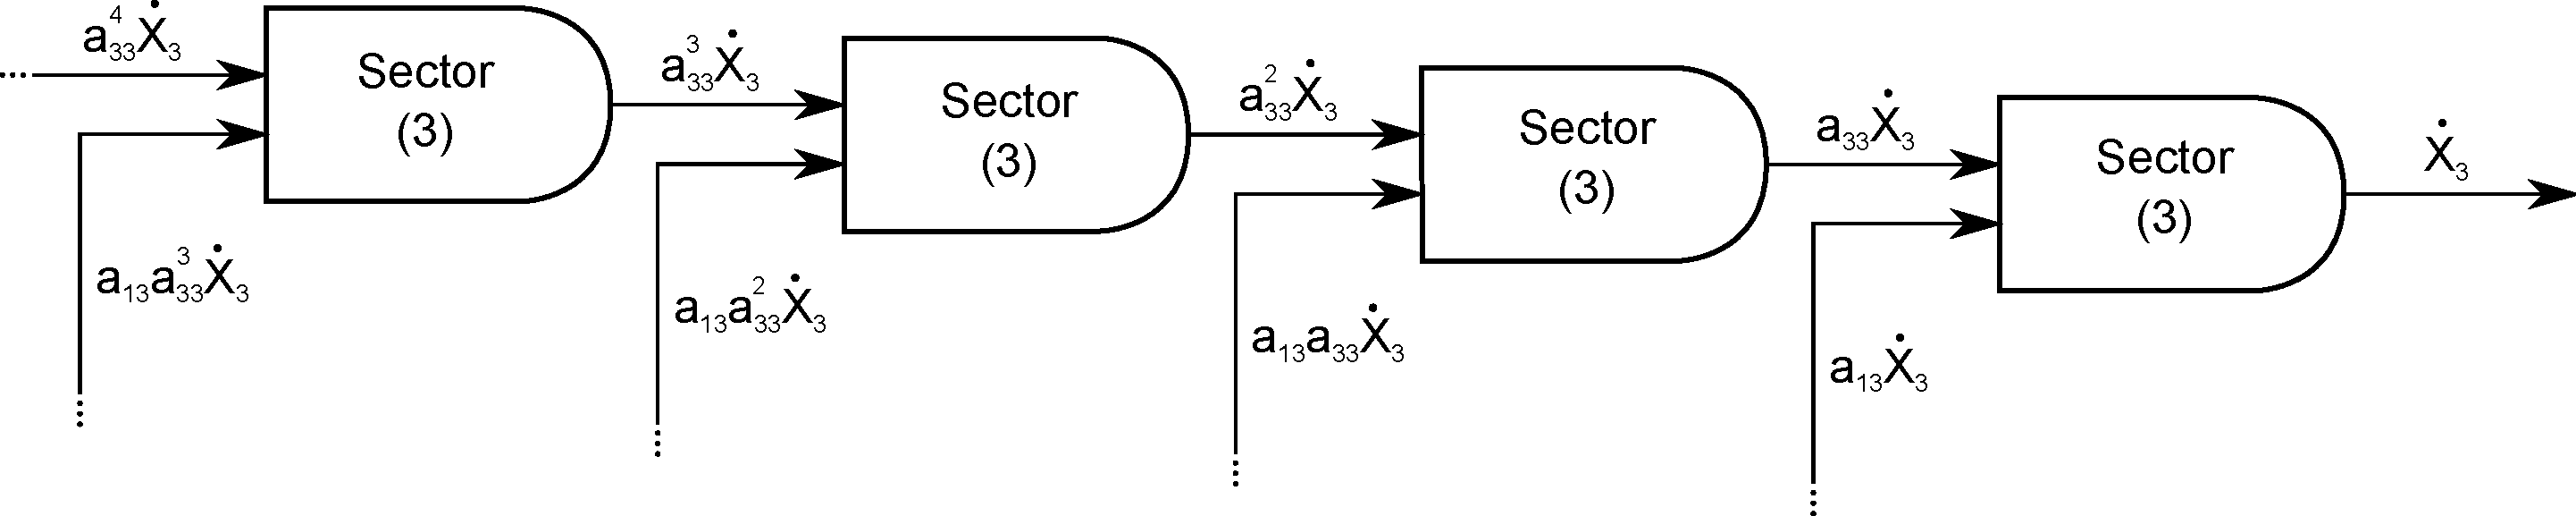
\includegraphics[width=1.0\linewidth]{images/Heun_I-O_Process_Equivalence_3.pdf}
\caption{Process flows in a single-sector economy.}
\label{fig:single_sector_flows_3}
\end{figure}

The economy produces output at a rate of $\dot{X}_{3}$, but it requires energy from the Earth ($\dot{E}_{13} = a_{13}\dot{X}_{3}$) to do so. The economy also consumes a fraction of its own gross output ($\dot{X}_{33} = a_{33}\dot{X}_{3}$). To produce $a_{33}\dot{X}_{3}$, the economy requires an additional $a_{13}a_{33}\dot{X}_{3}$ of energy from the Earth. The total energy required for the economy to produce at a rate of $\dot{X}_{3}$ is an infinite sum.

\begin{equation} \label{eq:E_dot_demand_SS}
	\dot{E}_{demand} = a_{13}\dot{X}_{3} + a_{13}a_{33}\dot{X}_{3} + a_{13}a_{33}^2\dot{X}_{3} + \cdots
\end{equation}

The energy intensity of the economy ($\varepsilon_{3}$) is 

\begin{equation} \label{eq:epsilon_process_SS_intermediate}
	\varepsilon_{3} = \frac{\dot{E}_{demand}}{\dot{X}_{3}} = a_{13}(1 + a_{33} + a_{33}^2) + \cdots = a_{13}\sum_{n=0}^{\infty}a_{33}^{n}.
\end{equation}

Realizing that $\sum_{n=0}^{\infty}a_{33}^{n} = \frac{1}{1-a_{33}}$ and $a_{13} = \frac{\dot{E}_{13}}{\dot{X}_{3}}$ gives

\begin{equation} \label{eq:epsilon_process_SS}
	\varepsilon_{1} = (1-a_{33})^{-1} \dot{X}^{-1} \dot{E}_{13}.
\end{equation}

Neglecting accumulation of embodied energy in the economy $\left(\frac{\mathrm{d}B_{3}}{\mathrm{d}t}\right)$ and depreciation $\left(\gamma_{3}B_{3}\right)$, Equations \ref{eq:eps3_ss_IO} and \ref{eq:epsilon_process_SS} are identical (assuming $\frac{\mathrm{d}B_{3}}{\mathrm{d}t} =\gamma_{3} = 0$), indicating that the I-O approach accounts for the infinite recursion of energy demand by the economy.


%%%%%%%%%%
\section{Example C: a two-sector economy}
%%%%%%%%%%

We extend single-sector Example B to derive a matrix representation for the I-O method that can be generalized to any number of economic sectors. A two-sector economy consisting of an Energy sector (3) and a Goods and Services sector (4) is considered. Both the Earth (1) and Society (2) are also included. Resources are extracted from the Earth (1), and Society (2) provides the final demand for both the Goods and Services (4) and the Energy (3) sectors.

%%%%%%%%%% Example C %%%%%%%%%%
\subsection{First Law of Thermodynamics}
%%%%%%%%%%

The First Law of Thermodynamics requires that energy is conserved around each sector of the economy as well as around the Earth (1) and Society (2) as shown in Figure \ref{fig:direct_energy_flows_2}. 

\begin{figure}[h!]
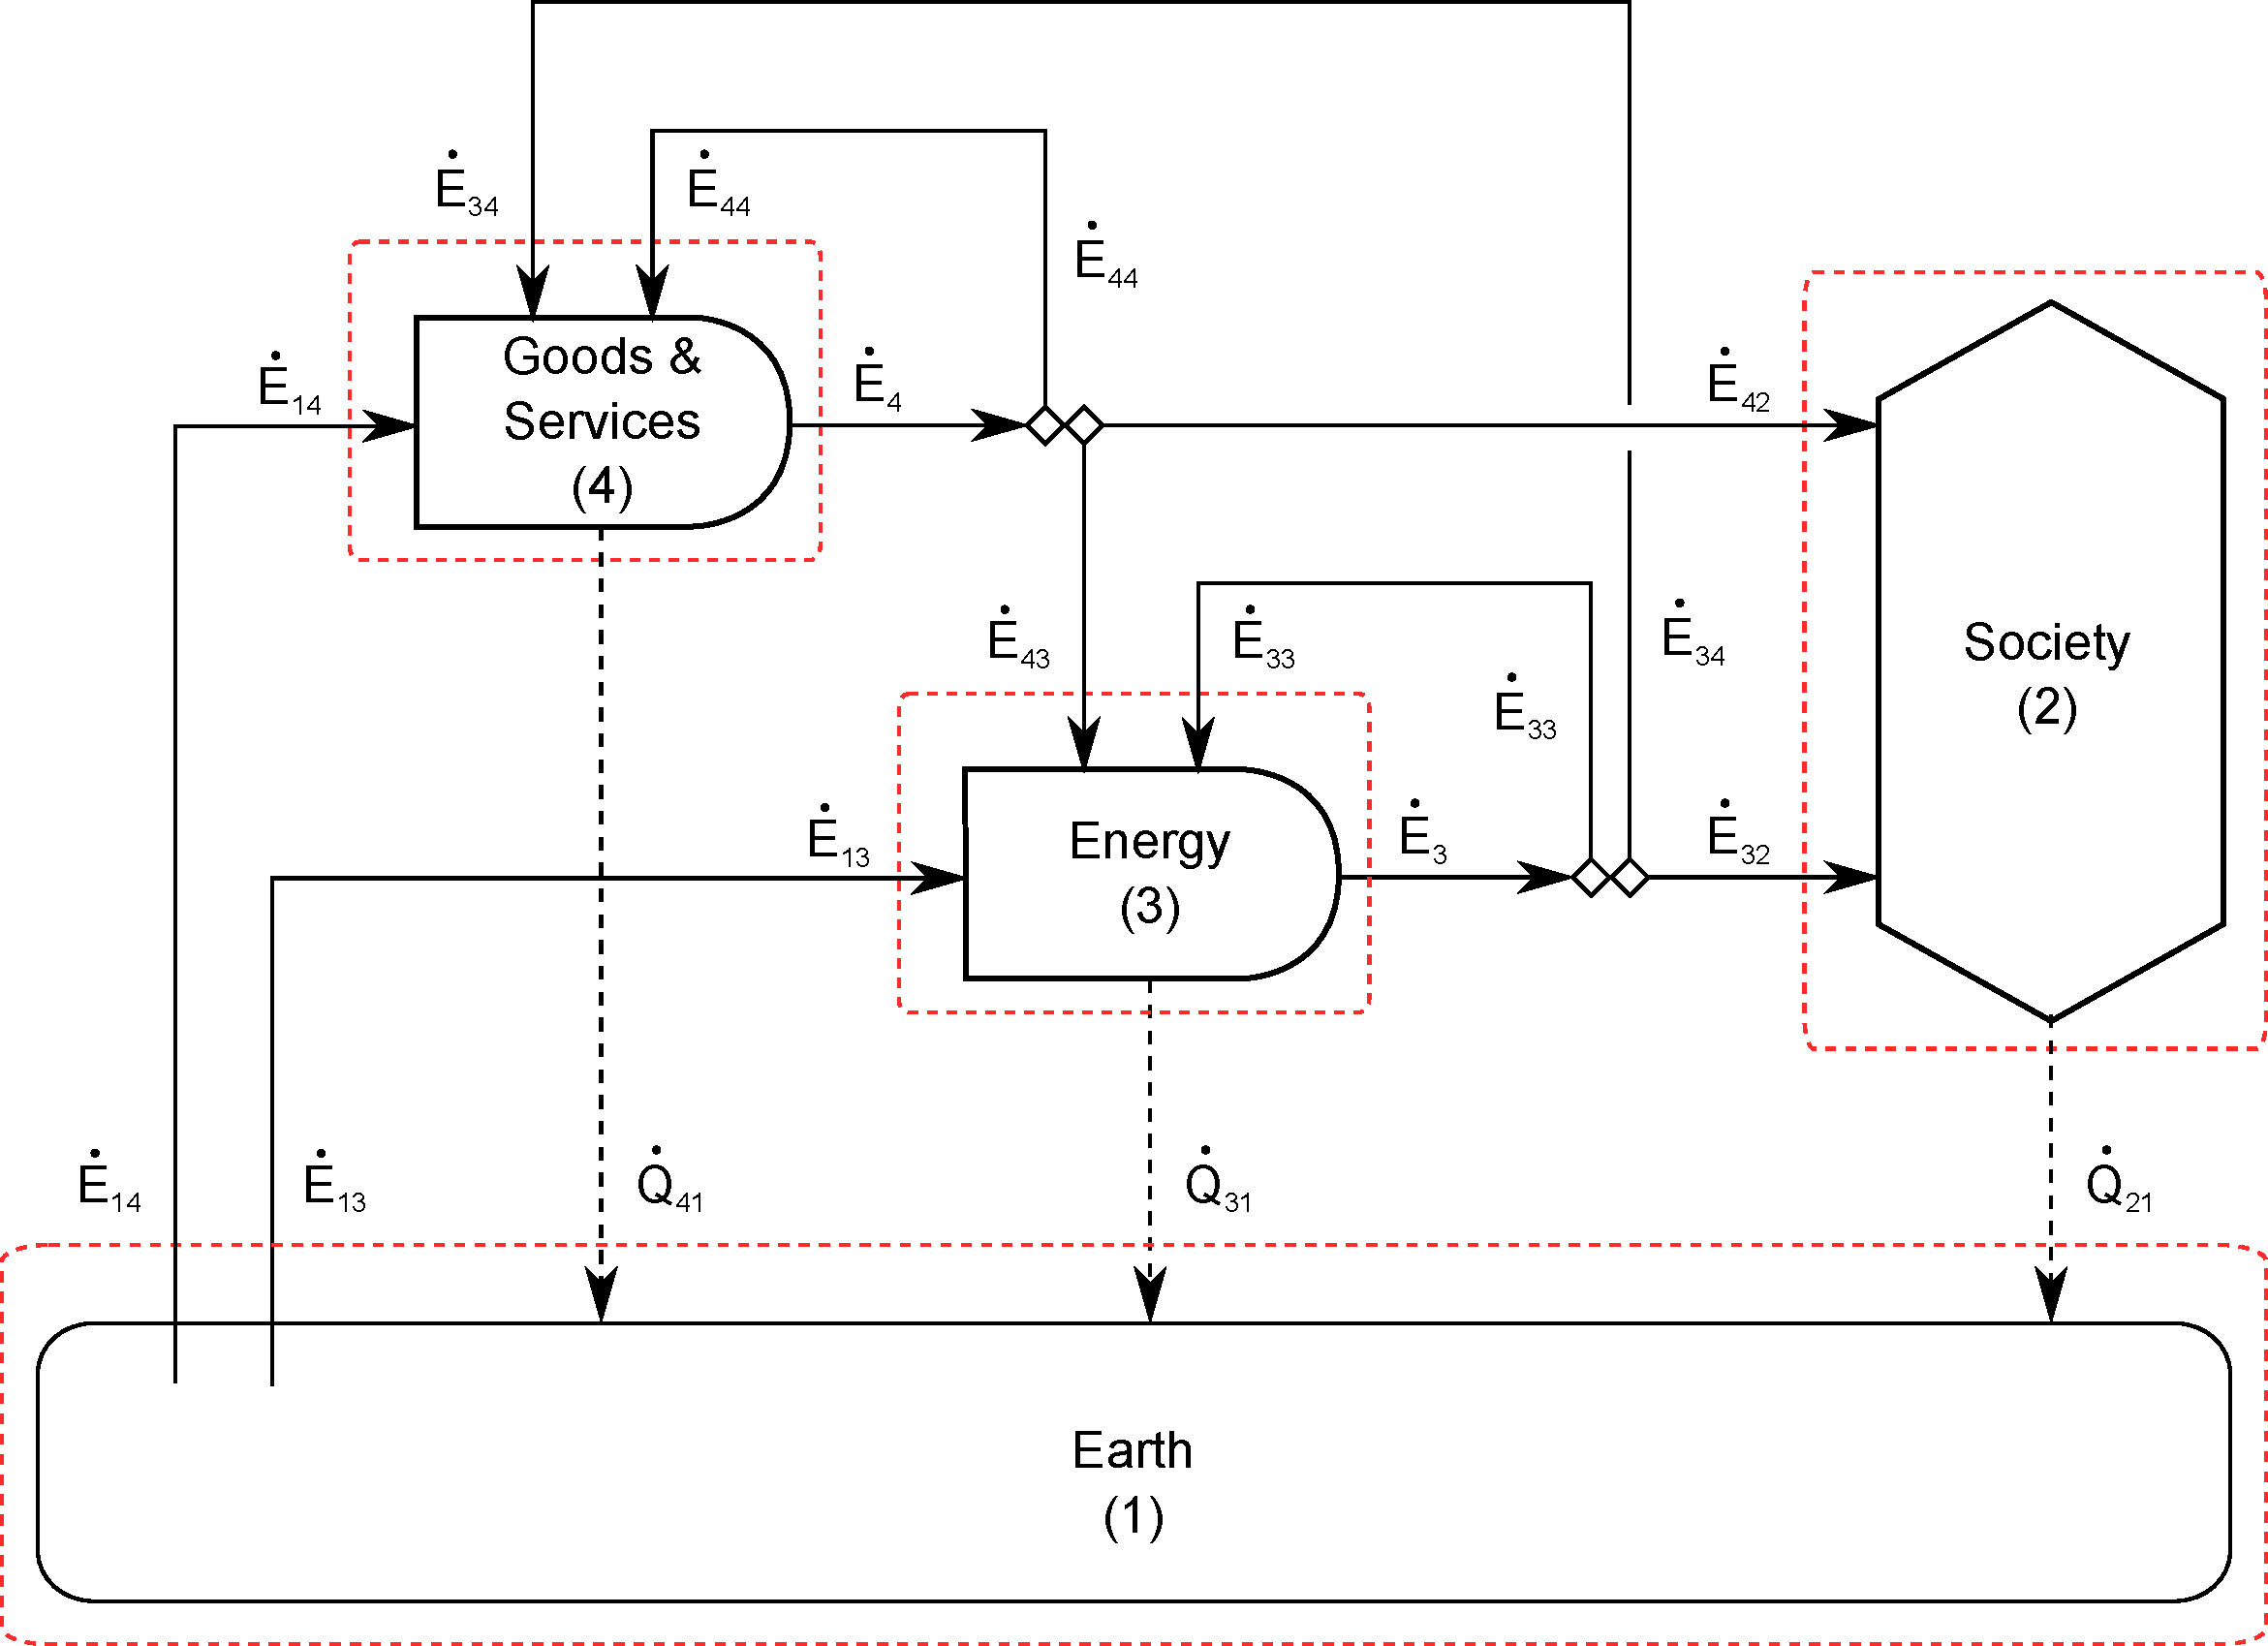
\includegraphics[width=1.0\linewidth]{images/I-O_three_sector_direct_energy.pdf}
\caption{Flows of direct energy ($\dot{E}$) and waste heat ($\dot{Q}$) in a two-sector economy.}
\label{fig:direct_energy_flows_2}
\end{figure}

In this economy, we assume that the purpose of the Goods and Services sector (4) is to produce goods and provide services, it provides no direct energy to society. The purpose of the Energy sector (3) is to make direct energy ($\dot{E}$) available to the economy and society in a useful form. Both direct energy ($\dot{E}$) (such as chemical potential energy in coal, oil, and electricity) and waste heat ($\dot{Q}$) are accounted by the First Law of Thermodynamics. The First Law around the Goods and Services sector (4) including, for now, the accumulation rate of direct energy in the sector $\left(\frac{\mathrm{d}E_{4}}{\mathrm{d}t}\right)$ yields

\begin{equation} \label{eq:C-CV_E_dot_4}
	\frac{\mathrm{d}E_{4}}{\mathrm{d}t} 	 =  \dot{E}_{14} + \dot{E}_{34} + \dot{E}_{44} - \dot{E}_4 - \dot{Q}_{41}.
\end{equation}

Note that we may simplify Equation \ref{eq:C-CV_E_dot_4} by realizing that $\dot{E}_{4} = \dot{E}_{4i} = 0$, because the goods and services sector is assumed to produce no flows of energy, and that $\dot{E}_{14} = 0$, since sector (4) receives no direct energy from the earth, except via the energy sector (3), hence:

\begin{equation} \label{eq:C-CV_E_dot_4_simp}
	\frac{\mathrm{d}E_{4}}{\mathrm{d}t} 	 =  \dot{E}_{34} - \dot{Q}_{41}.
\end{equation}

% [HOW DO WE WANT TO ACCOUNT FOR FOOD (i.e. ENERGY) OUTPUT FROM SECTOR (4) WHICH FLOWS INTO SECTOR (2) IN THIS FRAMEWORK? SIMILARLY, THERE ARE ENERGY FLOWS WHICH ARE USED INTERNALLY (E.G. FERTILIZERS, SO SHOULD WE HAVE $\dot{E}_{4}$ and $\dot{E}_{44}$ TERMS] 
% [ANOTHER CONCEPTUAL QUESTION IS WHETHER AN $\dot{E}_{24}$ TERM SHOULD BE INCLUDED. LABOR IS SUPPLIED FROM SOCIETY TO THE GOODS AND SERVICES SECTOR. LABOR IS A FORM OF DIRECT ENERGY, NO? --MKH]
% [FOOTNOTE ADDED TO DEAL WITH TWO COMMENTS ABOVE - MD]

%[I DECIDED TO INCLUDE THE $\dot{E_4}$ TERM IN THE ABOVE EQUATION. WE DON'T NEED AN $\dot{E}_{44}$ TERM. --MKH. I DON'T FOLLOW WHY WE DON'T NEED THE $\dot{E}_{44}$ TERM? - MD.]



The First Law of Thermodynamics around the Earth (1), Society (2), and the Energy sector (3) gives

\begin{equation} \label{eq:C-CV_E_dot_1}
	\frac{\mathrm{d}E_{1}}{\mathrm{d}t} 	 =  \dot{Q}_{21} + \dot{Q}_{31} + \dot{Q}_{41} - \dot{E}_{13} - \dot{E}_{14},
\end{equation}

\begin{equation} \label{eq:C-CV_E_dot_2}
	\frac{\mathrm{d}E_{2}}{\mathrm{d}t} 	 = \dot{E}_{32}  + \dot{E}_{42} - \dot{Q}_{21},
\end{equation}

\noindent and 

\begin{equation} \label{eq:C-CV_E_dot_3}
	\frac{\mathrm{d}E_{3}}{\mathrm{d}t} 	 = \dot{E}_{13} + \dot{E}_{33} + \dot{E}_{43} - \dot{E}_{3} - \dot{Q}_{31}.
\end{equation}

As in Examples A and B, we can set the accumulation of direct energy to zero.

\begin{equation} \label{eq:C-CV_E_dot_1_SS}
	0 =  \dot{Q}_{21} + \dot{Q}_{31} + \dot{Q}_{41} - \dot{E}_{13} - \dot{E}_{14}
\end{equation}

\begin{equation} \label{eq:C-CV_E_dot_2_SS}
	0  = \dot{E}_{32}  + \dot{E}_{42} - \dot{Q}_{21}
\end{equation}

\begin{equation} \label{eq:C-CV_E_dot_3_SS}
	0 = \dot{E}_{13} + \dot{E}_{33} + \dot{E}_{43} - \dot{E}_{3} - \dot{Q}_{31}
\end{equation}

\noindent and 

\begin{equation} \label{eq:C-CV_E_dot_4_SS}
	0 = \dot{E}_{14} + \dot{E}_{34} + \dot{E}_{44} - \dot{E}_4 - \dot{Q}_{41}
\end{equation}

%%%%%%%%%% Example C %%%%%%%%%%
\subsection{Total energy accounting}
%%%%%%%%%%

Again, we follow the I-O literature in assuming that total energy (i.e., the sum of direct energy and embodied energy) is conserved. Thus, we can draw a diagram similar to Figure \ref{fig:direct_energy_flows_2} for total energy flows.

\begin{figure}[h!]
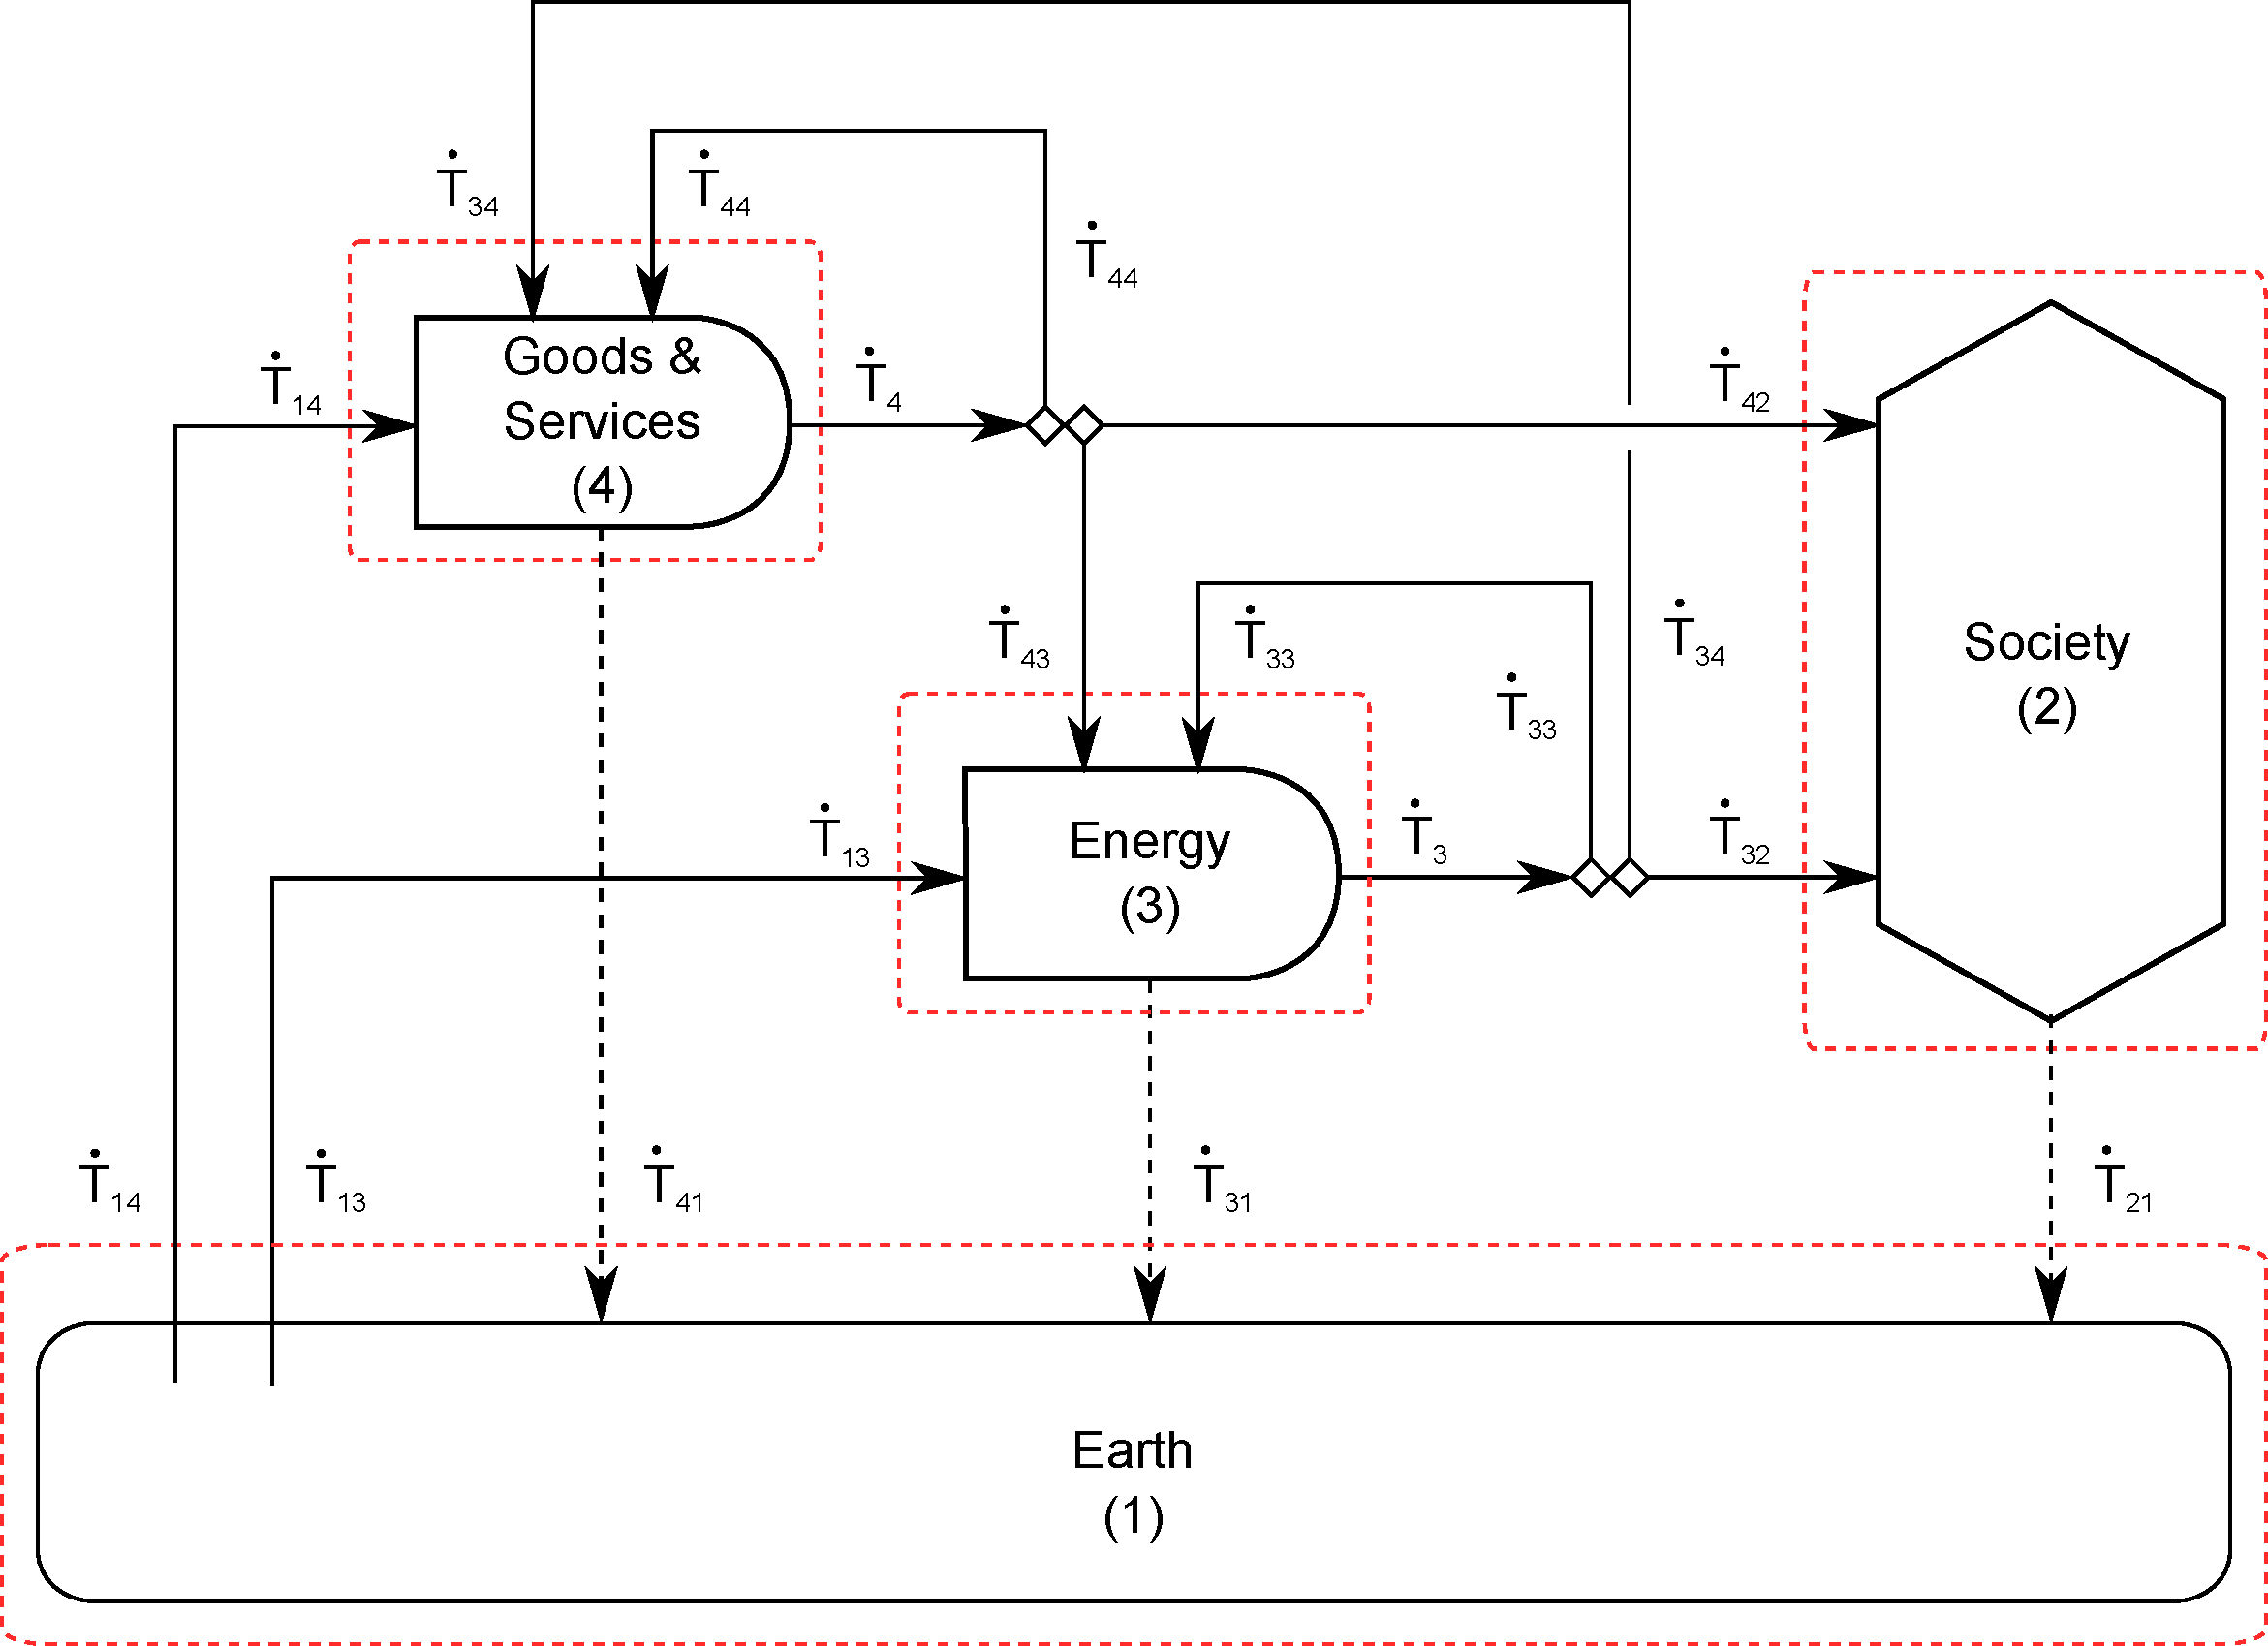
\includegraphics[width=1.0\linewidth]{images/I-O_three_sector_total_energy.pdf}
\caption{Flows of total energy ($\dot{T}$) in a two-sector economy.}
\label{fig:total_energy_flows_2S}
\end{figure}

Accounting for accumulation of total energy and using the assumption that total energy is conserved, we can write the following equations.

\begin{equation} \label{eq:C-CV_T_1}
	\frac{\mathrm{d}T_{1}}{\mathrm{d}t} 	 = \dot{T}_{21} + \dot{T}_{31} + \dot{T}_{41} - \dot{T}_{13} - \dot{T}_{14},
\end{equation}

\begin{equation} \label{eq:C-CV_T_2}
	\frac{\mathrm{d}T_{2}}{\mathrm{d}t} 	 = \dot{T}_{32} + \dot{T}_{42} - \dot{T}_{21},
\end{equation}

\begin{equation} \label{eq:C-CV_T_3}
	\frac{\mathrm{d}T_{3}}{\mathrm{d}t} 	 = \dot{T}_{13} + \dot{T}_{33} + \dot{T}_{43} - \dot{T}_{3} - \dot{T}_{31},
\end{equation}

\noindent and 

\begin{equation} \label{eq:C-CV_T_4}
	\frac{\mathrm{d}T_{4}}{\mathrm{d}t} 	 = \dot{T}_{14} + \dot{T}_{34} + \dot{T}_{44} - \dot{T}_{4} - \dot{T}_{41}.
\end{equation}

%%%%%%%%%% Example C %%%%%%%%%%
\subsection{Embodied energy accounting}
%%%%%%%%%%

Given that $\frac{\mathrm{d}E_{i}}{\mathrm{d}t} = 0$, we again note that $\frac{\mathrm{d}T_i}{\mathrm{d}t} = \frac{\mathrm{d}B_i}{\mathrm{d}t}$. Substituting $\dot{T} = \dot{E} + \dot{B}$ into the total energy accounting equations gives

\begin{equation} \label{eq:C-CV_dB_1}
	\frac{\mathrm{d}B_{1}}{\mathrm{d}t} 	 = \dot{E}_{21} + \dot{B}_{21} + \dot{E}_{31} + \dot{B}_{31} + \dot{E}_{41} + \dot{B}_{41} - \dot{E}_{13} - \dot{B}_{13} - \dot{E}_{14} - \dot{B}_{14},
\end{equation}

\begin{equation} \label{eq:C-CV_dB_2}
	\frac{\mathrm{d}B_{2}}{\mathrm{d}t} 	 = \dot{E}_{32} + \dot{B}_{32} + \dot{E}_{42} + \dot{B}_{42} - \dot{E}_{21} - \dot{B}_{21},
\end{equation}

\begin{equation} \label{eq:C-CV_dB_3}
	\frac{\mathrm{d}B_{3}}{\mathrm{d}t} 	 = \dot{E}_{13} + \dot{B}_{13} + \dot{E}_{33} + \dot{B}_{33} + \dot{E}_{43} + \dot{B}_{43} - \dot{E}_{3} - \dot{B}_{3} - \dot{E}_{31} - \dot{B}_{31},
\end{equation}

\noindent and 

\begin{equation} \label{eq:C-CV_dB_4}
	\frac{\mathrm{d}B_{4}}{\mathrm{d}t} 	 = \dot{E}_{14} + \dot{B}_{14} + \dot{E}_{34} + \dot{B}_{34} + \dot{E}_{44} + \dot{B}_{44} - \dot{E}_{4} - \dot{B}_{4} - \dot{E}_{41} - \dot{B}_{41}.
\end{equation}

Substituting the First Law of Thermodynamics (Equations \ref{eq:C-CV_E_dot_1_SS} through \ref{eq:C-CV_E_dot_4_SS}) into the total energy accounting equations (Equations \ref{eq:C-CV_dB_1} through \ref{eq:C-CV_dB_4}) gives embodied energy accounting equations for Example C.

\begin{equation} \label{eq:C-embodied_acct_1}
	\frac{\mathrm{d}B_{1}}{\mathrm{d}t} 	 = \dot{B}_{21} + \dot{B}_{31} + \dot{B}_{41} - \dot{B}_{13} - \dot{B}_{14} - \dot{Q}_{21} - \dot{Q}_{31} - \dot{Q}_{41}
\end{equation}

\begin{equation} \label{eq:C-embodied_acct_2}
	\frac{\mathrm{d}B_{2}}{\mathrm{d}t} 	 = \dot{B}_{32} + \dot{B}_{42} + \dot{Q}_{21} - \dot{B}_{21}
\end{equation}

\begin{equation} \label{eq:C-embodied_acct_3}
	\frac{\mathrm{d}B_{3}}{\mathrm{d}t} 	 = \dot{B}_{13} + \dot{B}_{33} + \dot{B}_{43} + \dot{Q}_{31} - \dot{B}_{3} - \dot{B}_{31}
\end{equation}

\begin{equation} \label{eq:C-embodied_acct_4}
	\frac{\mathrm{d}B_{4}}{\mathrm{d}t}	 = \dot{B}_{14} + \dot{B}_{34} + \dot{B}_{44} + \dot{Q}_{41} - \dot{B}_{4} - \dot{B}_{41}
\end{equation}

To verify the above derivation, we sum Equations \ref{eq:C-embodied_acct_1} through \ref{eq:C-embodied_acct_4} and use the following identities:

\begin{equation} \label{eq:C-B_sum_3_output}
	\dot{B}_3 = \dot{B}_{32} + \dot{B}_{33} + \dot{B}_{34}
\end{equation}

\noindent and

\begin{equation} \label{eq:C-B_sum_4_output}
	\dot{B}_4 = \dot{B}_{42} + \dot{B}_{43} + \dot{B}_{44};
\end{equation}

\noindent to obtain

\begin{equation} \label{eq:C-B_sums_to_zero}
	\frac{\mathrm{d}B_{1}}{\mathrm{d}t} + \frac{\mathrm{d}B_{2}}{\mathrm{d}t} + \frac{\mathrm{d}B_{3}}{\mathrm{d}t} + \frac{\mathrm{d}B_{4}}{\mathrm{d}t} = 0
\end{equation}

\noindent as expected. The total embodied energy content of the system (Earth (1), Society (2), Energy sector (3), and Goods and Services sector (4)) is constant with respect to time.


%%%%%%%%%% Example C %%%%%%%%%%
\subsection{Definition of embodied energy ($\dot{B}$)}\label{sec:embodied_energy}
%%%%%%%%%%

At this point we can develop a rigorous definition of embodied energy. To do so, we use the Goods and Services sector (4) from Example C. Direct energy accounting around the Goods and Services sector (Figure \ref{fig:direct_energy_flows_2}) yields

\begin{equation} \label{eq:CV_around_GS_sector_E_dot}
	\frac{\mathrm{d}E_{4}}{\mathrm{d}t} = \dot{E}_{14} + \dot{E}_{34} + \dot{E}_{44} - \dot{E}_{4} - \dot{Q}_{41},
\end{equation}

Total energy accounting around the Goods and Services sector (Figure \ref{fig:total_energy_flows_2S}) yields

\begin{equation} \label{eq:CV_around_GS_sector_T_dot}
	\frac{\mathrm{d}T_{4}}{\mathrm{d}t} = \dot{T}_{14} + \dot{T}_{34} + \dot{T}_{44} - \dot{T}_{4} + \dot{T}_{41},
\end{equation}

Solving the direct energy equation (Equation \ref{eq:CV_around_GS_sector_E_dot}) for the rate of direct energy input from the Energy sector (3) to the Goods and Services sector (4), namely $\dot{E}_{34}$, substituting into the total energy equation (Equation \ref{eq:CV_around_GS_sector_T_dot}), solving the result for $\dot{B}_{4}$, and assuming that no direct energy is wasted by the Goods and Services sector (4) to the Earth (1), i.e. $\dot{E}_{41} = 0$, yields

\begin{equation} \label{eq:embodied_output_GS}
	\dot{B}_{4} = \dot{B}_{14} + \dot{B}_{34} + \dot{B}_{44} + \dot{Q}_{41} - \frac{\mathrm{d}B_{4}}{\mathrm{d}t} - \dot{B}_{41}.
\end{equation}

Written generally, we obtain a formal definition for embodied energy output from an economic sector:

\begin{equation} \label{eq:embodied_def_1}
	\dot{B}_{j} \equiv \displaystyle\sum_{i} \dot{B}_{ij} - \frac{\mathrm{d}B_{j}}{\mathrm{d}t} - \dot{B}_{j1} + \dot{Q}_{j1}.
\end{equation}

Rearranging, we obtain

\begin{equation} \label{eq:embodied_def_2}
	\frac{\mathrm{d}B_{j}}{\mathrm{d}t} =  \displaystyle\sum_{i} \dot{B}_{ij} - \dot{B}_{j} - \dot{B}_{j1} + \dot{Q}_{j1}.
\end{equation}

In words, the rate of accumulation of embodied energy in a sector of the economy ($\frac{\mathrm{d}B_{j}}{\mathrm{d}t}$) is equal to the sum of the rates of input of embodied energy into the sector ($\displaystyle\sum_{i} \dot{B}_{ij}$) less the rate of useful output of embodied energy from the sector ($\dot{B}_{j}$) less  the rate of wasting embodied energy by the sector ($\dot{B}_{j1}$) \emph{plus} the rate of waste heat from the sector ($\dot{Q}_{j1}$). The first three terms on the right side of the equation are expected: accumulation is the difference between inflow and outflow rates. However, we see that the last term ($+\ \dot{Q}_{j1}$) in the above equations indicates that waste heat is \emph{additive} to both accumulation of embodied energy in a sector of the economy (Equation \ref{eq:embodied_def_2}) and outflow of embodied energy from a sector of the economy (Equation \ref{eq:embodied_def_1}). Furthermore, because the waste heat appears in the embodied energy output from a sector, waste heat accumulates along each step of a process such that the energy embodied in a finished product is the \emph{sum} of waste heats along a process path.


%%%%%%%%%% Example C %%%%%%%%%%
 \subsection{Depreciation}
%%%%%%%%%%

[SOMEWHERE WE NEED TO DISCUSS THE $\dot{S}_{i1}$ TERMS]

The terms $\dot{B}_{21}$,  $\dot{B}_{31}$, and $\dot{B}_{41}$ represent material depreciation (i.e., disposal) rates. As before, we can represent the embodied energy content of material depreciation as $\dot{B}_{i1} = \gamma_i B_i$ to obtain

\begin{equation} \label{eq:C-embodied_acct_1_depreciation}
	\frac{\mathrm{d}B_{1}}{\mathrm{d}t} 	 = \gamma_2 B_2 + \gamma_3 B_3 + \gamma_4 B_4 - \dot{B}_{13} - \dot{B}_{14} - \dot{Q}_{21} - \dot{Q}_{31} - \dot{Q}_{41}
\end{equation}

\begin{equation} \label{eq:C-embodied_acct_2_depreciation}
	\frac{\mathrm{d}B_{2}}{\mathrm{d}t} 	 = \dot{B}_{32} + \dot{B}_{42} + \dot{Q}_{21} - \gamma_2 B_2
\end{equation}

\begin{equation} \label{eq:C-embodied_acct_3_depreciation}
	\frac{\mathrm{d}B_{3}}{\mathrm{d}t} 	 = \dot{B}_{13} + \dot{B}_{33} + \dot{B}_{43} + \dot{Q}_{31} - \dot{B}_{3} - \gamma_3 B_3
\end{equation}

\begin{equation} \label{eq:C-embodied_acct_4_depreciation}
	\frac{\mathrm{d}B_{4}}{\mathrm{d}t}	 = \dot{B}_{14} + \dot{B}_{34} + \dot{B}_{44} + \dot{Q}_{41} - \dot{B}_{4} - \gamma_4 B_4
\end{equation}

%%%%%%%%%% Example C %%%%%%%%%%
%\subsection{Energy ratios}
%%%%%%%%%%%
%
%% [MIK: I MOVED THESE ENERGY RATIOS TO HERE FROM EARLIER, BECAUSE THEY NEED TO APPEAR AFTER WE DID THE TOTAL ENERGY ACCOUNTING FOR EXAMPLE C. YOU NEED TO REVIEW THIS SECTION IN LIGHT OF ALL OUR CHANGES. --MKH] 
%
%[THIS SECTION IS INTERESTING TO US, BUT MAY NOT BE GERMANE TO THE PAPER. IF THIS WERE TO BE A BOOK, I THINK WE SHOULD KEEP THIS SECTION IN. IF WE'RE NOW SHOOTING FOR A PAPER, WE CAN PROBABLY LEAVE THIS SECTION OUT. WE SHOULD AT LEAST REFERENCE THE LITERATURE HERE. OR, WE SHOULD MAKE USE OF THESE RATIOS. FOR EXAMPLE, IF WE WANT TO TALK ABOUT DECLINING RESOURCE QUALITY IN TERMS OF $EROI$ OR $GER$, WE SHOULD DO SO. WE SHOULD THEN SUBSTITUTE $GER$ INTO THE DERIVED EQUATIONS AND SHOW HOW A CHANGE IN $GER$ AFFECTS ENERGY FLOWS THROUGH THE ECONOMY.  --MKH]
%
%Several important energy ratios can be observed in Figure \ref{fig:direct_energy_flows_2}. [REFERENCE OTHER PAPERS FOR NOMENCLATURE? --MKH] The Gross Energy Ratio ($GER$) is defined as: 
%
%\begin{equation} \label{eq:C-GER_def}
%	GER_{\beta} \equiv \frac{\dot{E}_{3}}{\dot{E}_{33}}.
%\end{equation}
%
%\noindent The Net Energy Ratio ($NER$) is defined as [SHOULD THE NUMERATOR FOR $NER_\beta$ BE $\dot{E}_{32} + \dot{E}_{34}$? --MKH]
%
%[MIK SHOULD CHECK THE NEXT TWO EQUATIONS. ARE THEY CORRECT? --MKH]
%
%\begin{equation} \label{eq:NER_beta_def}
%	NER_{\beta} \equiv \frac{\dot{E}_{32}}{\dot{E}_{33}} = GER - 1.
%\end{equation}
%
%%[THESE DEFINITIONS ARE EQUIVALENT TO $\beta$ BOUNDARY DEFINED IN BRANDT AND DALE (2011). WE CAN DEFINE EXTERNAL ENERGY RATIO BY ACCOUNTING FOR TOTAL ENERGY FLOWS AS BELOW]
%
%[CAN WE SIMPLIFY THESE? FOR EXAMPLE, $\dot{E}_{43} = 0$, SO THE DENOMINATOR CAN BE SIMPLIFIED TO $\dot{B}_{43}$ --MKH]
%
%\begin{equation} \label{eq:C-GER_delta_def}
%	GER_{\delta} \equiv \frac{\dot{E}_{3}}{\dot{T}_{33} + \dot{T}_{43}};
%\end{equation}
%
%[THIS EQUATION DOESN'T LOOK RIGHT. IT IS SAME AS THE PREVIOUS EQUATION $GER - 1$, BUT HAS A DIFFERENT DENOMINATOR. MIK SHOULD CHECK. --MKH]
%\begin{equation} \label{eq:C-NER_delta_def}
%	NER_{\beta} \equiv \frac{\dot{E}_{32} + \dot{E}_{34}}{\dot{T}_{33} + \dot{T}_{43}} = GER - 1;
%\end{equation}
%
%We may also define a Gross External Energy Ratio (GEER) and Net External Energy Ratio (NEER), which account only for inputs from other sectors in the denominator:
%
%\begin{equation} \label{eq:C-GEER_delta_def}
%	GEER_{\delta} \equiv \frac{\dot{E}_{3}}{\dot{T}_{43}},
%\end{equation}
%
%and
%
%\begin{equation} \label{eq:C-NEER_delta_def}
%	NEER_{\beta} \equiv \frac{\dot{E}_{32}}{\dot{T}_{43}}.
%\end{equation}

%%%%%%%%%% Example C %%%%%%%%%%
\subsection{Final demand}
%%%%%%%%%%

Society's demand vector for total energy, $\dot{T}$, can be written as 

\begin{equation} \label{eq:demand_vector_T_dot}
	\vec{Y}_{\dot{T}} = 	\begin{Bmatrix} 	\dot{T}_{32}	\\
																\dot{T}_{42}	\\
									\end{Bmatrix}.
\end{equation}

\noindent In terms of total energy, the ultimate demand ($Y_{\dot{T}}$) is given by 

\begin{equation} \label{eq:final_demand_T_sum}
	Y_{\dot{T}} = 	\sum_{i=3}^{N} \dot{T}_{i2} = \dot{T}_{32} + \dot{B}_{42}.
\end{equation}

\noindent after realizing that $\dot{E}_{42} = 0$. 

[IS THE FOLLOWING PARAGRAPH IN THE RIGHT PLACE?]

We acknowledge that there are examples in the real economy which run counter to this model, where output from non-energy sectors are valued for their energetic content, one example being agriculture.  ``Direct'' energy inputs also flow in the opposite direction in the form of labor, which we also neglect. This will serve to introduce errors which will be small for industrial economies and larger for less industrial societies. To illustrate this we may compare the United States with India. To feed an adult requires around 2000 kcal/day $\approx$ 3 GJ/yr. To feed the whole $\sim$300 million population of the States requires around 1$\times 10^{18}$J (1 EJ) which is around 1\% of the roughly 100 EJ of primary energy supply. The US labor force currently stands at around 240 million. Given that a human can supply around 100 W of power and assuming an 8 hour work day, the US labor force will supply 70 TWh/yr $\approx$ 0.25 EJ. For India, the energy to food to feed 1.25 billion people is nearly 4 EJ which is around 15\% of the $\sim$25 EJ of primary energy consumed. Assuming that the labor force makes up 500 million people working at 12 hours per day, the energy supplied by labor is around 0.8 EJ or around 3\% of the total primary energy. As such, we can see that food energy accounts for around 1\% of primary energy in the US and around 15\% in India. Similarly, the labor inputs account for around 0.25\% in the US and around 3\% in India. The implication of including or omitting these flows is different in each case. Our assumptions introduce small errors for industrial societies where most of the world's energy is consumed.

Using $\dot{T}_{32} = \dot{E}_{32} + \dot{B}_{32}$ and rearranging Equation \ref{eq:final_demand_T_sum} gives

\begin{equation} \label{eq:rearranged_final_demand_T_sum}
	\dot{B}_{32} + \dot{B}_{42} = Y_{\dot{T}} - \dot{E}_{32}.
\end{equation}

\noindent Substituting Equation \ref{eq:rearranged_final_demand_T_sum} into Equation \ref{eq:C-embodied_acct_2_depreciation} yields

\begin{equation} \label{eq:intermediate_T_sum_dB2_dt}
	\frac{\mathrm{d}B_2}{\mathrm{d}t} = Y_{\dot{T}} - \dot{E}_{32} + \dot{Q}_{21} - \gamma_2 B_2.
\end{equation}

Substituting Equation \ref{eq:C-CV_E_dot_2_SS} into Eqaution \ref{eq:intermediate_T_sum_dB2_dt} and realizing that $\dot{E}_{42} = 0$ because direct energy is supplied to society by the energy sector only, we obtain 

\begin{equation} \label{eq:compare_demand_and_accumulation}
	\frac{\mathrm{d}B_{2}}{\mathrm{d}t} = Y_{\dot{T}} - \gamma_{2}B_{2},
\end{equation}

[IT WOULD BE GOOD TO FIND SOME VERY ROUGH DATA FOR THIS VALUE, E.G. WHAT IS THE AVERAGE LIFETIME OF MANUFACTURED GOODS - INCLUDING PACKAGING AND NON-CONSUMER GOODS. WHAT IS THE BALANCE OF NON-DURABLE VS. DURABLE GOODS? WHAT PROPORTION OF GOODS (E.G. FOOD) IS WASTED BEFORE EVER BEING CONSUMED?]

[I AGREE. HOW? --MKH]

\noindent indicating that the final demand vector for total energy ($Y_{\dot{T}}$) and the accumulation rate of energy in society $\left(\frac{\mathrm{d}B_{2}}{\mathrm{d}t}\right)$ differ by the rate of disposal from society ($\gamma_{2}B_{2}$). We note that as total embodied energy in society ($B_{2}$) becomes increasingly large, we need an ever-increasing rate of energy supplied to the society ($Y_{\dot{T}}$) to maintain positive growth $\left(\frac{\mathrm{d}B_{2}}{\mathrm{d}t}\right)$. [MAIN POINT THAT MUST BE DISCUSSED IN FURTHER DETAIL LATER, PARTICULARLY IN RELATION TO INCREASING GDP NOT NECESSARILY SIGNALING INCREASING ACCUMULATION OR GROWTH.]

%[WE NEVER USE THE FINAL PARAGRAPHS OF THIS SECTION. I PROPOSE THAT WE DELETE THEM. --MKH]
%
%A control volume around the economy gives
%
%\begin{equation} \label{eq:CV_around_economy_B_dot}
%	Y_{\dot{B}} = \sum_{j=1}^{N} \dot{E}_{1j} - \sum_{i=1}^{N} \dot{B}_{i1} - \dot{Q}_{21},
%\end{equation}
%
%[I HAVE ADDED $\dot{Q}_{21}$ TERM HERE, AS THERE IS DEFINITELY WASTE HEAT FROM CONSUMPTION OF FINAL ENERGY $Y_{\dot{B}}$ THAT IS NOT EMBODIED IN GOOD OR SERVICE, E.G. THE ELECTRICITY I USE TO COOK MY DINNER, OR WATCH TV]
%
%\noindent illustrating that final demand to society ($Y_{\dot{B}}$) can be considered the ultimate energy sink in the absence of depreciation in the economy.
%
%It is also interesting to note that 
%
%\begin{equation} \label{eq:flow_more_than_demand}
%	\sum_{i=1}^{N} \dot{T}_{i} > Y_{\dot{T}},
%\end{equation}
%
%\noindent which is a consequence of the self-demand of sectors within the economy.

%%%%%%%%%% Example C %%%%%%%%%%
\subsection{Flows of Value ($\dot{X}$)}
%%%%%%%%%%

The following figure shows value flows ($\dot{X}$) in the two-sector economy.

\begin{figure}[h!]
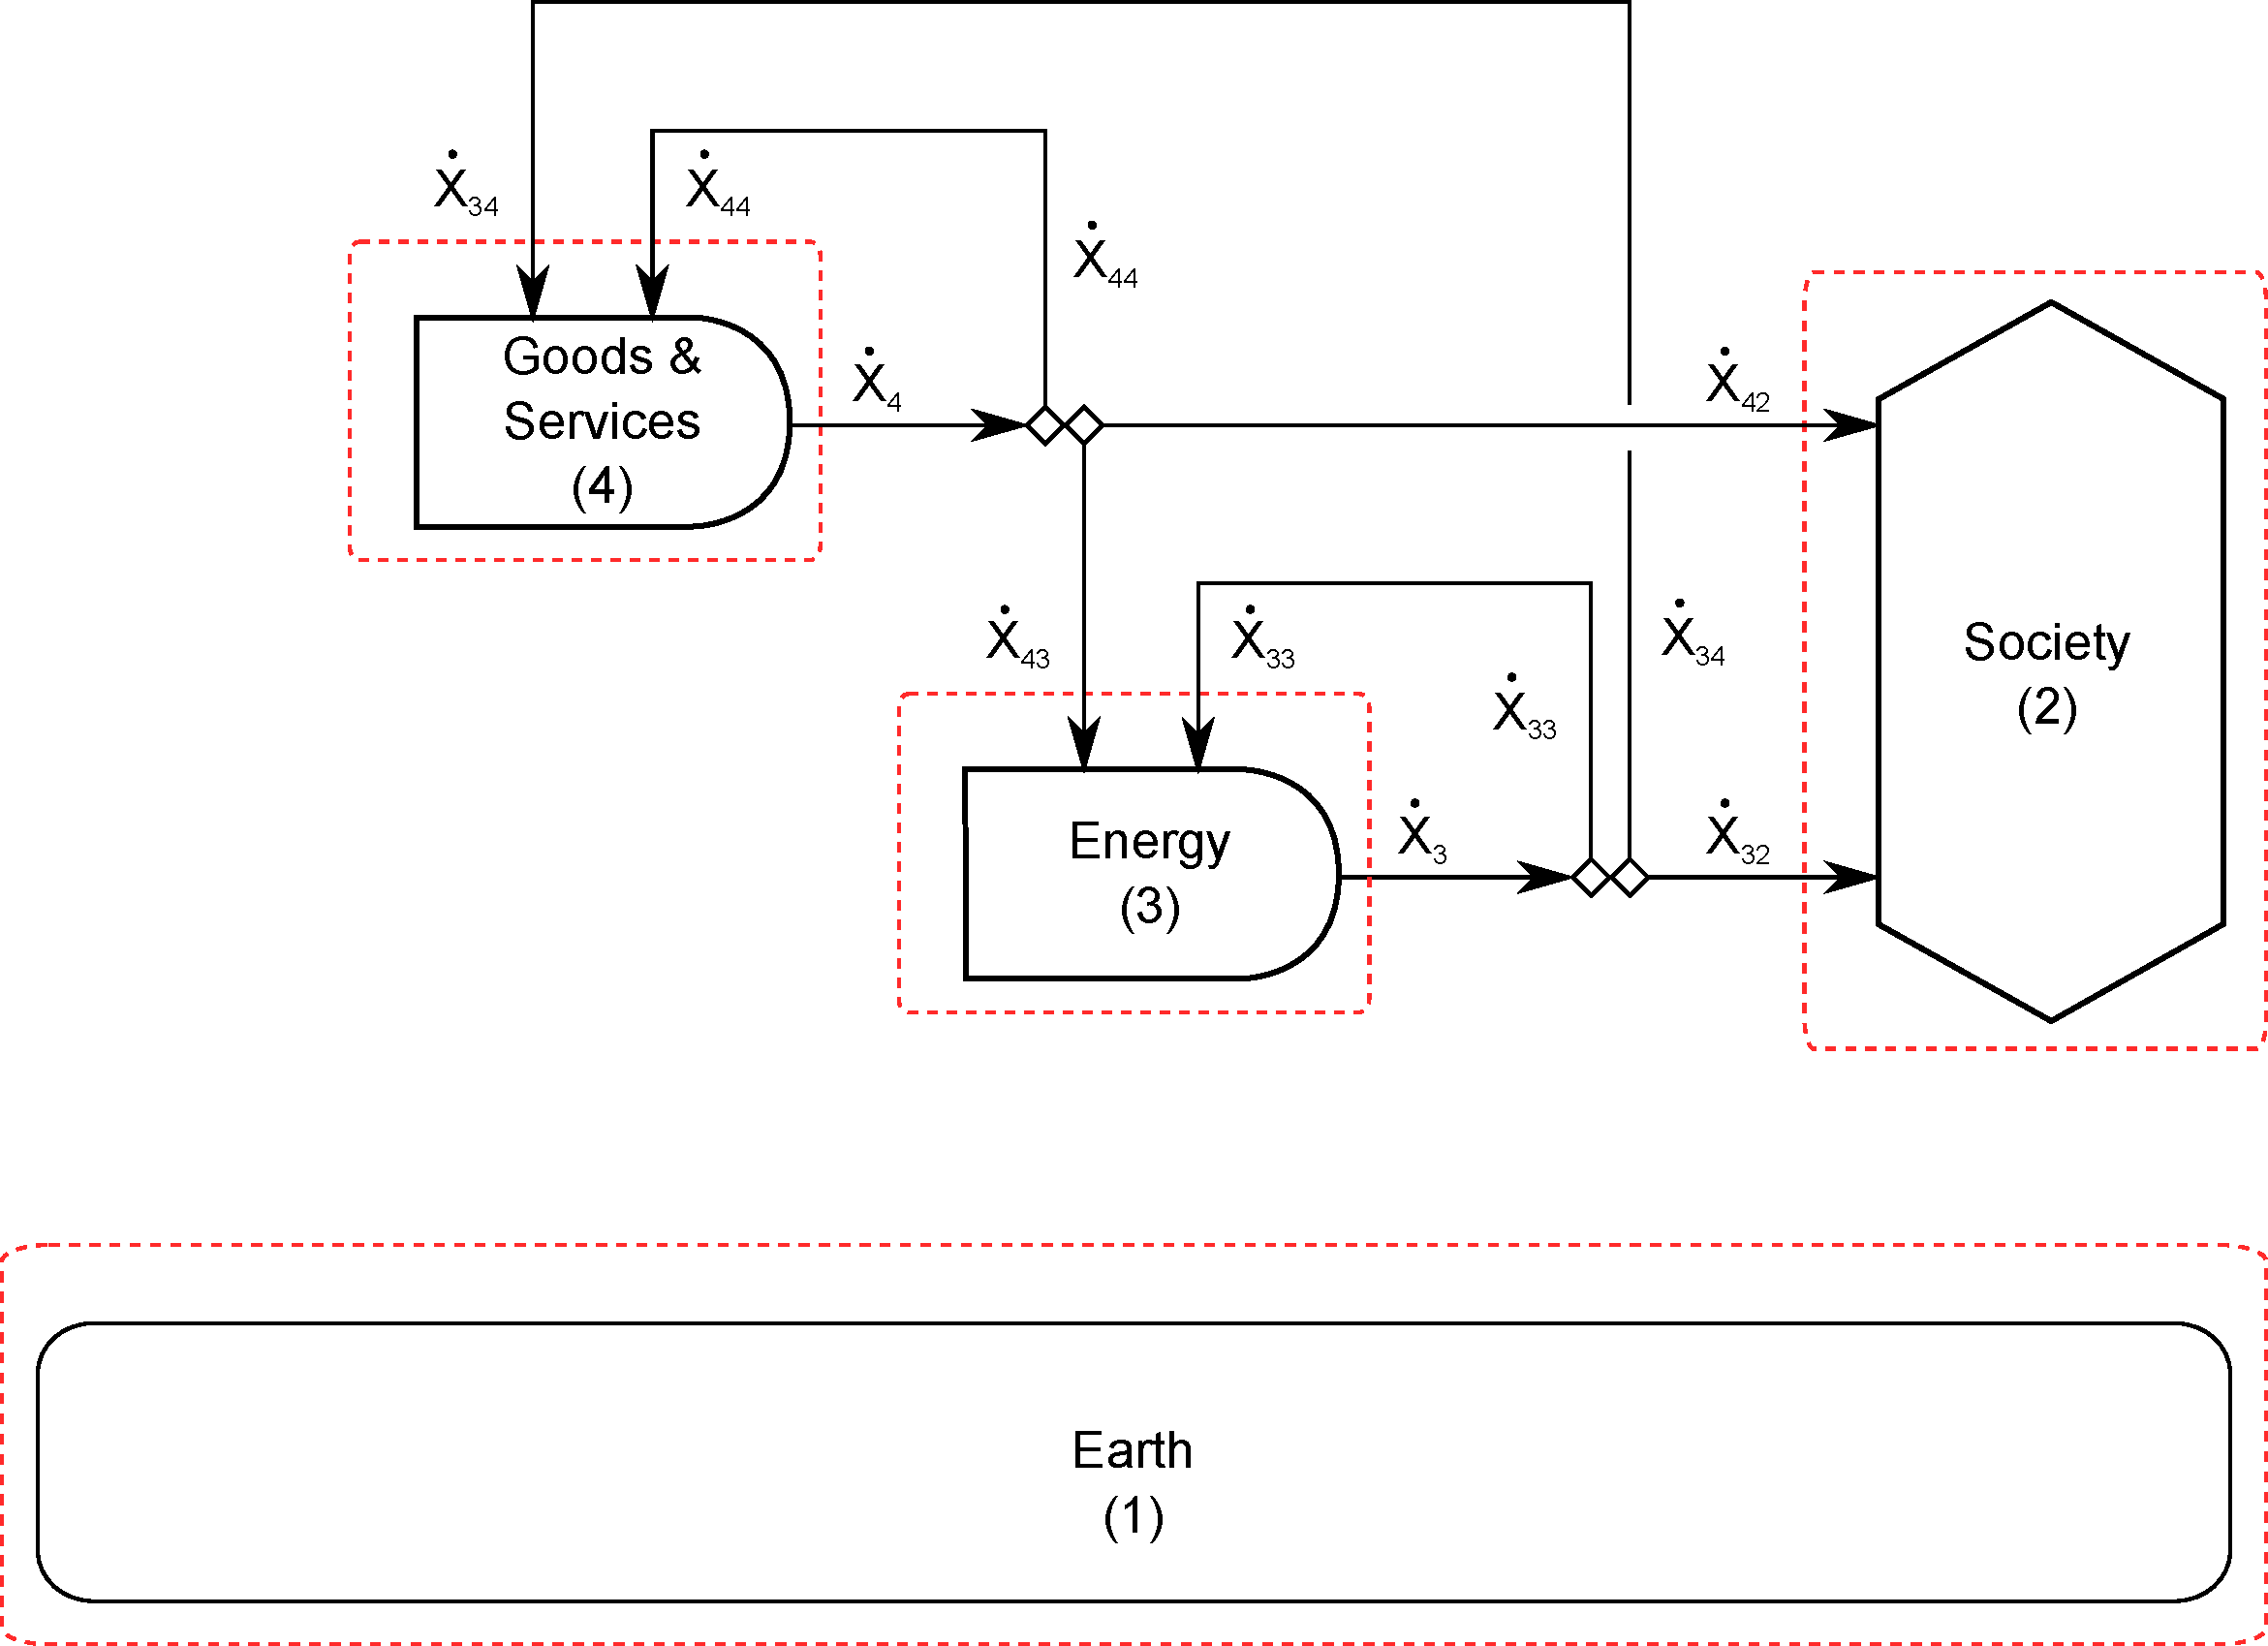
\includegraphics[width=1.0\linewidth]{images/I-O_three_sector_value.pdf}
\caption{Flows of economic value ($\dot{X}$) in a two-sector economy.}
\label{fig:economic_value_flows_2}
\end{figure}

Realizing that the valuable output from energy sectors is direct energy, $\dot{X}_{3} = \dot{E}_{3}$ and $\dot{X}_{3j} = \dot{E}_{3j}$. Thus, outputs from energy sectors are given in energy units (joules or BTUs). 

%With reference to Equations \ref{eq:GER_def_ch_5} and \ref{eq:NER_def_ch_5}, we can express the Gross Energy Ratio ($GER$) and Net Energy Ratio ($NER$) as
%
%\begin{equation} \label{eq:GER_in_terms_of_a_2}
%	GER_{\gamma} = \frac{\dot{E}_{3}}{\dot{E}_{33}} = \frac{\dot{X}_{3}}{\dot{X}_{33}} = \frac{1}{a_{33}},
%\end{equation}
%
%\noindent and
%
%\begin{equation} \label{eq:NER_in_terms_of_a_2}
%	NER = GER - 1 = \frac{1}{a_{33}} - 1.
%\end{equation}
%
%[DO WE NEED THESE NEXT TWO EQUATIONS? DO WE USE THEM ANYWHERE? THEY MIGHT BE HELPFUL FOR A GDP DISCUSSION, BUT WE HAVEN'T INCLUDED THAT DISCUSSION YET. --MKH]

Written in terms of value flows, the ultimate demand vector ($\vec{Y}$) is given by

\begin{equation} \label{eq:demand_vector_B_dot}
	\vec{Y}_{\dot{X}} = 	\begin{Bmatrix} 	\dot{X}_{32}	\\
																\dot{X}_{42}	\\
									\end{Bmatrix},
\end{equation}

\noindent and the total value demand from society ($Y$) is 

\begin{equation} \label{eq:total_value_demand}
	Y_{\dot{X}} = \sum_{i=1}^{N} \dot{X}_{i2} = \dot{X}_{32} + \dot{X}_{42}.
	\end{equation}


%%%%%%%%%% Example C %%%%%%%%%%
\subsection{Matrix Formulation}
%%%%%%%%%%

We can use Equations \ref{eq:epsilon_output_def} through \ref{eq:epsilon_equiv_1} to rewrite Equations \ref{eq:C-CV_B_1_depreciation} and \ref{eq:C-CV_B_2_depreciation} as

\begin{equation} \label{eq:CV_B_3_with_eps}
	\dot{X}_{33}\varepsilon_{3} + \dot{X}_{43}\varepsilon_{4} + \dot{E}_{13} - \frac{\mathrm{d}B_{3}}{\mathrm{d}t} - \gamma_{3}B_{3} = \dot{X}_{3}\varepsilon_{3}
\end{equation}

\noindent and 

\begin{equation} \label{eq:CV_B_4_with_eps}
	\dot{X}_{34}\varepsilon_{3} + \dot{X}_{44}\varepsilon_{4} + \dot{E}_{14} - \frac{\mathrm{d}B_{4}}{\mathrm{d}t} - \gamma_{4}B_{4} = \dot{X}_{4}\varepsilon_{4}.
\end{equation}

We can rewrite Equations \ref{eq:CV_B_3_with_eps} and \ref{eq:CV_B_4_with_eps} in matrix notation with the following definitions:

\begin{equation} \label{eq:eps_vec_def}
	\vec{\varepsilon} =		\begin{Bmatrix} 	\varepsilon_{3}	\\
																\varepsilon_{4}	\\
									\end{Bmatrix},
\end{equation}

\begin{equation} \label{eq:E_vec_def}
	\vec{E} =		\begin{Bmatrix} 	\dot{E}_{13}	\\
													\dot{E}_{14}\\
						\end{Bmatrix},
\end{equation}

\begin{equation} \label{eq:dBdt_vec_def}
	\frac{\mathrm{d}\vec{B}}{\mathrm{d}t} =	\begin{Bmatrix}	\frac{\mathrm{d}B_{3}}{\mathrm{d}t}	\\
																									\frac{\mathrm{d}B_{4}}{\mathrm{d}t}\\
																		\end{Bmatrix},
\end{equation}

\begin{equation} \label{eq:B_vec_def}
	\vec{B} =			\begin{Bmatrix}	B_{3}\\
														B_{4}\\
							\end{Bmatrix},
\end{equation}

\begin{equation} \label{eq:A_matrix_def}
	\vec{A} =	\begin{bmatrix} 	a_{33} & a_{34}	\\
												a_{43} & a_{44}	\\
					\end{bmatrix},
\end{equation}

\begin{equation} \label{eq:X_t_matrix_def}
	\vec{X}_{t} =		\begin{bmatrix} 	\dot{X}_{33}		&	\dot{X}_{34}	\\
														\dot{X}_{43}		&	\dot{X}_{44}\\
							\end{bmatrix},
\end{equation}

\begin{equation} \label{eq:X_hat_matrix_def}
	\hat{\vec{X}} = \delta_{ij}\dot{X}_{j} = \begin{bmatrix} 	\dot{X}_{33}		&	0					\\
																								0					&	\dot{X}_{44}	\\
																							\end{bmatrix},
\end{equation}

\begin{equation} \label{eq:B_hat_matrix_def}
	\hat{\vec{\gamma}} = \delta_{ij}\gamma_{j},
\end{equation}

[CAN WE MAKE THIS EQUATION EXPLICIT]

\noindent and

\begin{equation}\label{eq:k_delta}
	\delta_{ij} = \begin{cases}	1 	& 	\text{if  } i = j		\\
												0	&	\text{if  } i \neq j	\\
						\end{cases},
\end{equation}

\noindent such that:

\begin{equation} \label{eq:matrix_leontief}
	\vec{X}_{t}^{\mathrm{T}}\vec{\varepsilon} + \vec{E} - \left(\frac{\mathrm{d}\vec{B}}{\mathrm{d}t} + \hat{\vec{\gamma}}\vec{B}\right) = \hat{\vec{X}}\vec{\varepsilon}.
\end{equation}

Additional relationships that will be helpful later include (derived in Appendix):

\begin{equation} \label{eq:Xhat_X_and_A}
	\hat{\vec{X}}^{-1}\vec{X}_{t} = \vec{A}^{\mathrm{T}},
\end{equation}

\begin{equation} \label{eq:Xdifference1}
	\vec{X}_{t}^{\mathrm{T}} - \hat{\vec{X}} = \hat{\vec{X}}(\vec{A}^{\mathrm{T}} - \vec{I}),
\end{equation}

\begin{equation} \label{eq:Xdifference2}
	\hat{\vec{X}} - \vec{X}_{t}^{\mathrm{T}} = \hat{\vec{X}}(\vec{I} - \vec{A}^{\mathrm{T}}),
\end{equation}

\noindent and

\begin{equation} \label{eq:Xdifference2_inverse}
	\left(\hat{\vec{X}} - \vec{X}_{t}^{\mathrm{T}}\right)^{-1} = (\vec{I} - \vec{A}^{\mathrm{T}})^{-1}\hat{\vec{X}}^{-1}.
\end{equation}


%%%%%%%%%% Example C %%%%%%%%%%
\subsection{Estimating $\vec{\varepsilon}$ and $\frac{\mathrm{d}\vec{B}}{\mathrm{d}t}$}
%%%%%%%%%%

With Equation \ref{eq:matrix_leontief}, we can solve for either the energy accumulation vector ($\vec{\frac{\mathrm{d}B}{\mathrm{d}t}}$) or the energy intensity vector ($\vec{\varepsilon}$), but not both. 

Solving for the accumulation vector gives

\begin{equation} \label{eq:dB_dt_leontief}
	\frac{\mathrm{d}\vec{B}}{\mathrm{d}t} = (\vec{X}_{t}^{\mathrm{T}} - \hat{\vec{X}})\vec{\varepsilon} + \vec{E} - \hat{\vec{\gamma}}\vec{B}.
\end{equation}

\noindent Finally, we can substutute Equation \ref{eq:Xdifference1} which gives

\begin{equation} \label{eq:dB_dt_leontief_with_A}
	\frac{\mathrm{d}\vec{B}}{\mathrm{d}t} = \hat{\vec{X}} (\vec{A}^{\mathrm{T}} - \vec{I}) \vec{\varepsilon} + \vec{E} - \hat{\vec{\gamma}}\vec{B},
\end{equation}

\noindent which allows estimation of the embodied energy accumulation in economic sectors $\left(\frac{\mathrm{d}\vec{B}}{\mathrm{d}t}\right)$ knowing only sector outputs ($\hat{\vec{X}}$), sector input-output ratios ($\vec{A}$), sector energy intensities ($\vec{\varepsilon}$), energy input to the economy ($\vec{E}$), and sector physical depreciation rates ($\hat{\vec{\gamma}}\vec{b}$). In theory, the transaction matrix ($\vec{X}_{t}$) is not required if the input-ouput ratios ($\vec{A}$) are known, though in reality, knowledge of input-output ratios would be derived from the transaction matrix $\vec{X}_{t}$ .

Solving for the energy intensity vector gives

\begin{equation} \label{eq:epsilon_leontief}
	\vec{\varepsilon} = (\hat{\vec{X}} - \vec{X}_{t}^{\mathrm{T}})^{-1}\left[\vec{E} - \left(\frac{\mathrm{d}\vec{B}}{\mathrm{d}t} + \hat{\vec{\gamma}}\vec{B}\right)\right].
\end{equation}

\noindent Substituting Equation \ref{eq:Xdifference2_inverse} gives

\begin{equation} \label{eq:epsilon_leontief_with_A}
	\vec{\varepsilon} = (\vec{I} - \vec{A}^{\mathrm{T}})^{-1}\hat{\vec{X}}^{-1}\left[\vec{E} - \left(\frac{\mathrm{d}\vec{B}}{\mathrm{d}t} + \hat{\vec{\gamma}}\vec{B}\right)\right],
\end{equation}

\noindent which allows estimation of the energy intensity of economic sectors ($\vec{\varepsilon}$) knowing only sector input-output ratios ($\vec{A}$), sector outputs ($\hat{\vec{X}}$), energy input to the economy ($\vec{E}$), sector embodied energy accumulation rates $\left(\frac{\mathrm{d}\vec{B}}{\mathrm{d}t}\right)$, and sector physical depreciation rates ($\hat{\vec{\gamma}}\vec{B}$).

Comparison of Equations \ref{eq:eps1_ss_IO} and \ref{eq:epsilon_leontief_with_A} shows the similarities between the single-sector algebraic formulation and the multi-sector matrix formulation of the I-O analysis method. This newly developed multi-sector matrix formulation can be extended to any desired level of economic and energy sector disaggregation as shown by Bullard (1975, 1978) and others.

************************** MATT ENDED HERE *************************

%%%%%%%%%%
\section{Example D: a two-sector economy with durable and non-durable goods}
%%%%%%%%%%

We now extend the two-sector economy from Example C by distinguishing two types of embodied energy flows: short-lived, non-durable goods (S), such as packaging, newspapers or the embodied content of direct energy flows and long-lived, durable goods (L), such as appliances, capital equipment, roads or buildings. In reality, (as the names suggest) the distinction between short- and long-lived goods is really one of degree rather than a difference in kind, as we are making, such that the distribution in lifetime of goods stretches from a matter of hours or days for some intermediate goods right up to thousands of years for some structures still in use today \cite{Leask2012}. We assume that there is no accumulation of short-lived goods within the economy or society, such that $\frac{\textrm{d}S}{\textrm{dt}} = 0$.  We can define the following relationships:

\begin{equation}\label{eq:D_def_S_L}
B \equiv S + L = L
\end{equation}

\begin{equation}\label{eq:D_def_dot_S_L}
\dot{B} = \dot{S} + \dot{L}
\end{equation}

\begin{equation}\label{eq:D_def_acc_S_L}
\frac{\textrm{d}B}{\textrm{dt}} =\frac{\textrm{d}S}{\textrm{dt}} + \frac{\textrm{d}L}{\textrm{dt}} = \frac{\textrm{d}L}{\textrm{dt}}
\end{equation}

%%%%%%%%%% Example D %%%%%%%%%%
\subsection{First Law of Thermodynamics}
%%%%%%%%%%

As before, the First Law of Thermodynamics requires that energy is conserved around each sector of the economy as well as around the Earth (1) and Society (2) as shown in Figure \ref{fig:direct_energy_flows_2}. All of the direct energy flows remain as they were for Example C, outlined in Equations \ref{eq:C-CV_E_dot_4} - \ref{eq:C-CV_E_dot_4_SS}.

%%%%%%%%%% Example D %%%%%%%%%%
\subsection{Total energy accounting}
%%%%%%%%%%

Again, the total energy accounting equations remain the same for this new Example D, as they were for Example C outlined in Equations \ref{eq:C-CV_T_1} - \ref{eq:C-CV_T_4}.

%%%%%%%%%% Example D %%%%%%%%%%
\subsection{Embodied energy accounting}
%%%%%%%%%%

Given that $\frac{\mathrm{d}E_{i}}{\mathrm{d}t} = \frac{\mathrm{d}S_{i}}{\mathrm{d}t} = 0$, we again note that $\frac{\mathrm{d}T_i}{\mathrm{d}t} = \frac{\mathrm{d}B_i}{\mathrm{d}t} = \frac{\mathrm{d}L_{i}}{\mathrm{d}t}$. Substituting $\dot{T} = \dot{E} + \dot{B} = \dot{E} + \dot{S} + \dot{L}$ into the total energy accounting equations gives

\begin{equation} \label{eq:D-CV_dB_1}
	\frac{\mathrm{d}L_{1}}{\mathrm{d}t} 	 = \dot{E}_{21} + \dot{S}_{21} + \dot{L}_{21}+ \dot{E}_{31} + \dot{S}_{31} + \dot{L}_{31} + \dot{E}_{41} + \dot{S}_{41} + \dot{L}_{41} - \dot{E}_{13} - \dot{S}_{13} - \dot{L}_{13} - \dot{E}_{14} - \dot{S}_{14} - \dot{L}_{14},
\end{equation}

\begin{equation} \label{eq:D-CV_dB_2}
	\frac{\mathrm{d}L_{2}}{\mathrm{d}t} 	 = \dot{E}_{32} + \dot{S}_{32} + \dot{L}_{32} + \dot{E}_{42} + \dot{S}_{42} + \dot{L}_{42} - \dot{E}_{21} - \dot{S}_{21} - \dot{L}_{21},
\end{equation}

\begin{equation} \label{eq:D-CV_dB_3}
	\frac{\mathrm{d}L_{3}}{\mathrm{d}t} 	 = \dot{E}_{13} + \dot{S}_{13} + \dot{L}_{13} + \dot{E}_{33} + \dot{S}_{33} + \dot{L}_{33}+ \dot{E}_{43} + \dot{S}_{43} + \dot{L}_{43} - \dot{E}_{3} - \dot{S}_{3} - \dot{L}_{3} - \dot{E}_{31} - \dot{S}_{31} - \dot{L}_{31},
\end{equation}

\noindent and 

\begin{equation} \label{eq:D-CV_dB_4}
	\frac{\mathrm{d}L_{4}}{\mathrm{d}t} 	 = \dot{E}_{14} + \dot{S}_{14} + \dot{L}_{14} + \dot{E}_{34} + \dot{S}_{34} + \dot{L}_{34}+ \dot{E}_{44} + \dot{S}_{44} + \dot{L}_{44} - \dot{E}_{4} - \dot{S}_{4} - \dot{L}_{4} - \dot{E}_{41} - \dot{S}_{41} - \dot{L}_{41}.
\end{equation}

Substituting the First Law of Thermodynamics (Equations \ref{eq:C-CV_E_dot_1_SS} through \ref{eq:C-CV_E_dot_4_SS}) into the total energy accounting equations (Equations \ref{eq:D-CV_dB_1} through \ref{eq:D-CV_dB_4}) gives embodied energy accounting equations for Example D.

\begin{equation} \label{eq:D-embodied_acct_1}
	\frac{\mathrm{d}L_{1}}{\mathrm{d}t} 	 = \dot{S}_{21} + \dot{L}_{21} + \dot{S}_{31} + \dot{L}_{31} + \dot{S}_{41} + \dot{L}_{41} - \dot{S}_{13} - \dot{L}_{13} - \dot{S}_{14} -  \dot{L}_{14} - \dot{Q}_{21} - \dot{Q}_{31} - \dot{Q}_{41}
\end{equation}

\begin{equation} \label{eq:D-embodied_acct_2}
	\frac{\mathrm{d}L_{2}}{\mathrm{d}t} 	 = \dot{S}_{32} +  \dot{L}_{32} + \dot{S}_{42} +  \dot{S}_{42} + \dot{Q}_{21} - \dot{S}_{21} -  \dot{L}_{21}
\end{equation}

\begin{equation} \label{eq:D-embodied_acct_3}
	\frac{\mathrm{d}L_{3}}{\mathrm{d}t} 	 = \dot{S}_{13} +  \dot{L}_{13} + \dot{S}_{33} +  \dot{L}_{33} + \dot{S}_{43} +  \dot{S}_{43} + \dot{Q}_{31} - \dot{S}_{3} -  \dot{L}_{3} - \dot{S}_{31} -  \dot{L}_{31}
\end{equation}

\begin{equation} \label{eq:D-embodied_acct_4}
	\frac{\mathrm{d}L_{4}}{\mathrm{d}t}	 = \dot{S}_{14} +  \dot{L}_{14} + \dot{S}_{34} +  \dot{L}_{34} + \dot{S}_{44} +  \dot{L}_{44} + \dot{Q}_{41} - \dot{S}_{4} -  \dot{L}_{4} - \dot{S}_{41} -  \dot{L}_{41}
\end{equation}

To verify the above derivation, we sum Equations \ref{eq:D-embodied_acct_1} through \ref{eq:D-embodied_acct_4} and use the following identities:

\begin{equation} \label{eq:D-S_sum_3_output}
	\dot{S}_3 = \dot{S}_{32} + \dot{S}_{33} + \dot{S}_{34}
\end{equation}

\begin{equation} \label{eq:D-L_sum_3_output}
	\dot{L}_3 = \dot{L}_{32} + \dot{L}_{33} + \dot{L}_{34}
\end{equation}

\begin{equation} \label{eq:D-S_sum_4_output}
	\dot{S}_4 = \dot{S}_{42} + \dot{S}_{43} + \dot{S}_{44};
\end{equation}

\noindent and

\begin{equation} \label{eq:D-L_sum_4_output}
	\dot{L}_4 = \dot{L}_{42} + \dot{L}_{43} + \dot{L}_{44};
\end{equation}

\noindent to obtain

\begin{equation} \label{eq:D-B_sums_to_zero}
	\frac{\mathrm{d}B_{1}}{\mathrm{d}t} + \frac{\mathrm{d}B_{2}}{\mathrm{d}t} + \frac{\mathrm{d}B_{3}}{\mathrm{d}t} + \frac{\mathrm{d}B_{4}}{\mathrm{d}t} = 0
\end{equation}

\noindent as expected. The total embodied energy content of the system (Earth (1), Society (2), Energy sector (3), and Goods and Services sector (4)) is constant with respect to time.

%%%%%%%%%% Example D %%%%%%%%%%
 \subsection{Depreciation}
%%%%%%%%%%

The terms $\dot{L}_{21}$,  $\dot{L}_{31}$, and $\dot{L}_{41}$ represent material depreciation (i.e., disposal) rates. We can represent the embodied energy content of material depreciation as $\dot{L}_{i1} = \gamma_i L_i$. Realizing that $S_i = 0$ we can see that $\gamma_i L_i = \gamma_i B_i$ which we may use to obtain:

\begin{equation} \label{eq:D-embodied_acct_1_depreciation}
	\frac{\mathrm{d}L_{1}}{\mathrm{d}t} 	 = \dot{S}_{21} + \gamma_2 B_2 + \dot{S}_{31} + \gamma_3 B_3 + \dot{S}_{41} + \gamma_4 B_4 - \dot{S}_{13} - \dot{L}_{13} - \dot{S}_{14} - \dot{L}_{14} - \dot{Q}_{21} - \dot{Q}_{31} - \dot{Q}_{41}
\end{equation}

\begin{equation} \label{eq:D-embodied_acct_2_depreciation}
	\frac{\mathrm{d}L_{2}}{\mathrm{d}t} 	 = \dot{S}_{32} + \dot{L}_{32} + \dot{S}_{42} + \dot{L}_{42} + \dot{Q}_{21} - \dot{S}_{21} - \gamma_2 B_2
\end{equation}

\begin{equation} \label{eq:D-embodied_acct_3_depreciation}
	\frac{\mathrm{d}L_{3}}{\mathrm{d}t} 	 = \dot{S}_{13} + \dot{L}_{13} + \dot{S}_{33} + \dot{L}_{33} + \dot{S}_{43} + \dot{L}_{43} + \dot{Q}_{31} - \dot{S}_{3} - \dot{L}_{3} - \dot{S}_{31} - \gamma_3 B_3
\end{equation}

\begin{equation} \label{eq:D-embodied_acct_4_depreciation}
	\frac{\mathrm{d}L_{4}}{\mathrm{d}t}	 = \dot{S}_{14} + \dot{L}_{14} + \dot{S}_{34} + \dot{L}_{34} + \dot{S}_{44} + \dot{L}_{44} + \dot{Q}_{41} - \dot{S}_{4} - \dot{L}_{4} - \dot{S}_{41} - \gamma_4 B_4
\end{equation}


%%%%%%%%%% Example D %%%%%%%%%%
\subsection{Final demand}
%%%%%%%%%%

Society's demand vector for total energy, $\dot{T}$, can again be written as 

\begin{equation} \label{eq:D-demand_vector_T_dot}
	\vec{Y}_{\dot{T}} = 	\begin{Bmatrix} 	\dot{T}_{32}	\\
																\dot{T}_{42}	\\
									\end{Bmatrix}.
\end{equation}

\noindent In terms of total energy, the ultimate demand ($Y_{\dot{T}}$) is given by 

\begin{equation} \label{eq:D-final_demand_T_sum}
	Y_{\dot{T}} = 	\sum_{i=3}^{N} \dot{T}_{i2} = \dot{T}_{32} + \dot{B}_{42} = \dot{T}_{32} + \dot{S}_{42} + \dot{L}_{42}.
\end{equation}

\noindent after realizing that $\dot{E}_{42} = 0$.

Using $\dot{T}_{32} = \dot{E}_{32} + \dot{S}_{32} + \dot{L}_{32}$ and rearranging Equation \ref{eq:D-final_demand_T_sum} gives

\begin{equation} \label{eq:D-rearranged_final_demand_T_sum}
	\dot{S}_{32} +\dot{L}_{32} + \dot{S}_{42} + \dot{L}_{42} = Y_{\dot{T}} - \dot{E}_{32}.
\end{equation}

\noindent Substituting Equation \ref{eq:D-rearranged_final_demand_T_sum} into Equation \ref{eq:D-embodied_acct_2_depreciation} yields

\begin{equation} \label{eq:D-intermediate_T_sum_dB2_dt}
	\frac{\mathrm{d}L_2}{\mathrm{d}t} = Y_{\dot{T}} - \dot{E}_{32} + \dot{Q}_{21} - \dot{S}_{21} - \gamma_2 B_2.
\end{equation}

Substituting Equation \ref{eq:D-CV_E_dot_2_SS} into Eqaution \ref{eq:D-intermediate_T_sum_dB2_dt} and realizing that $\dot{E}_{42} = 0$ because direct energy is supplied to society by the energy sector only, we obtain 

\begin{equation} \label{eq:D-compare_demand_and_accumulation}
	\frac{\mathrm{d}L_{2}}{\mathrm{d}t} = Y_{\dot{T}} - \dot{S}-{21} - \gamma_{2}B_{2},
\end{equation}

\noindent indicating that the final demand vector for total energy ($Y_{\dot{T}}$) and the accumulation rate of energy in society $\left(\frac{\mathrm{d}L_{2}}{\mathrm{d}t}\right)$ differ by the rate of disposal from society ($\gamma_{2}B_{2}$). We note that as total embodied energy in society ($B_{2}$) becomes increasingly large, we need an ever-increasing rate of energy supplied to the society ($Y_{\dot{T}}$) to maintain positive growth $\left(\frac{\mathrm{d}L_{2}}{\mathrm{d}t}\right)$. 

%%%%%%%%%% Example D %%%%%%%%%%
\subsection{Flows of Value ($\dot{X}$)}
%%%%%%%%%%

The following figure shows value flows ($\dot{X}$) in the two-sector economy.

Realizing that the valuable output from energy sectors is direct energy, $\dot{X}_{3} = \dot{E}_{3}$ and $\dot{X}_{3j} = \dot{E}_{3j}$. Thus, outputs from energy sectors are given in energy units (joules or BTUs). 

Written in terms of value flows, the ultimate demand vector ($\vec{Y}$) is given by

\begin{equation} \label{eq:D-demand_vector_B_dot}
	\vec{Y}_{\dot{X}} = 	\begin{Bmatrix} 	\dot{X}_{32}	\\
																\dot{X}_{42}	\\
									\end{Bmatrix},
\end{equation}

\noindent and the total value demand from society ($Y$) is 

\begin{equation} \label{eq:D-total_value_demand}
	Y_{\dot{X}} = \sum_{i=1}^{N} \dot{X}_{i2} = \dot{X}_{32} + \dot{X}_{42}.
	\end{equation}

%%%%%%%%%% Example D %%%%%%%%%%
\subsection{Matrix Formulation}
%%%%%%%%%%

We can use Equations \ref{eq:epsilon_output_def} through \ref{eq:epsilon_equiv_1} to rewrite Equations \ref{eq:D-CV_B_1_depreciation} and \ref{eq:D-CV_B_2_depreciation} as

\begin{equation} \label{eq:D-CV_B_3_with_eps}
	\dot{X}_{33}\varepsilon_{3} + \dot{X}_{43}\varepsilon_{4} + \dot{E}_{13} - \frac{\mathrm{d}L_{3}}{\mathrm{d}t} - \dot{S}_{31} - \gamma_{3}B_{3} = \dot{X}_{3}\varepsilon_{3}
\end{equation}

\noindent and 

\begin{equation} \label{eq:D-CV_B_4_with_eps}
	\dot{X}_{34}\varepsilon_{3} + \dot{X}_{44}\varepsilon_{4} + \dot{E}_{14} - \frac{\mathrm{d}L_{4}}{\mathrm{d}t} - \dot{S}_{41} - \gamma_{4}B_{4} = \dot{X}_{4}\varepsilon_{4}.
\end{equation}

We can rewrite Equations \ref{eq:D-CV_B_3_with_eps} and \ref{eq:D-CV_B_4_with_eps} in matrix notation with the following definitions:

\begin{equation} \label{eq:D-eps_vec_def}
	\vec{\varepsilon} =		\begin{Bmatrix} 	\varepsilon_{3}	\\
																\varepsilon_{4}	\\
									\end{Bmatrix},
\end{equation}

\begin{equation} \label{eq:D-E_vec_def}
	\vec{E} =		\begin{Bmatrix} 	\dot{E}_{13}	\\
													\dot{E}_{14}\\
						\end{Bmatrix},
\end{equation}

\begin{equation} \label{eq:D-dLdt_vec_def}
	\frac{\mathrm{d}\vec{L}}{\mathrm{d}t} =	\begin{Bmatrix}	\frac{\mathrm{d}L_{3}}{\mathrm{d}t}	\\
																									\frac{\mathrm{d}L_{4}}{\mathrm{d}t}\\
																		\end{Bmatrix},
\end{equation}

\begin{equation} \label{eq:B_vec_def}
	\vec{B} =	\vec{L} =		\begin{Bmatrix}	B_{3}\\
																	B_{4}\\
										\end{Bmatrix},
\end{equation}

\begin{equation} \label{eq:D-A_matrix_def}
	\vec{A} =	\begin{bmatrix} 	a_{33} & a_{34}	\\
												a_{43} & a_{44}	\\
					\end{bmatrix},
\end{equation}

\begin{equation} \label{eq:D-X_t_matrix_def}
	\vec{X}_{t} =		\begin{bmatrix} 	\dot{X}_{33}		&	\dot{X}_{34}	\\
														\dot{X}_{43}		&	\dot{X}_{44}\\
							\end{bmatrix},
\end{equation}

\begin{equation} \label{eq:D-X_hat_matrix_def}
	\hat{\vec{X}} = \delta_{ij}\dot{X}_{j} = \begin{bmatrix} 	\dot{X}_{33}		&	0					\\
																								0					&	\dot{X}_{44}	\\
																							\end{bmatrix},
\end{equation}


\begin{equation} \label{eq:D-B_hat_matrix_def}
	\hat{\vec{\gamma}} = \delta_{ij}\gamma_{j},
\end{equation}

\noindent and

\begin{equation} \label{eq:D-S_vec_def}
	\vec{S} =		\begin{Bmatrix} 	\dot{E}_{31}	\\
													\dot{E}_{41}\\
						\end{Bmatrix},
\end{equation}

\noindent such that:

\begin{equation} \label{D-eq:matrix_leontief}
	\vec{X}_{t}^{\mathrm{T}}\vec{\varepsilon} + \vec{E} - \left(\frac{\mathrm{d}\vec{L}}{\mathrm{d}t} +\vec{S} + \hat{\vec{\gamma}}\vec{L}\right) = \hat{\vec{X}}\vec{\varepsilon}.
\end{equation}

%%%%%%%%%% Example D %%%%%%%%%%
\subsection{Estimating $\vec{\varepsilon}$ and $\frac{\mathrm{d}\vec{B}}{\mathrm{d}t}$}
%%%%%%%%%%

With Equation \ref{eq:D-matrix_leontief}, we can solve for either the energy accumulation vector ($\vec{\frac{\mathrm{d}L}{\mathrm{d}t}}$) or the energy intensity vector ($\vec{\varepsilon}$), but not both. 

Solving for the accumulation vector gives

\begin{equation} \label{eq:D-dL_dt_leontief}
	\frac{\mathrm{d}\vec{L}}{\mathrm{d}t} = (\vec{X}_{t}^{\mathrm{T}} - \hat{\vec{X}})\vec{\varepsilon} + \vec{E} - \vec{S} - \hat{\vec{\gamma}}\vec{B}.
\end{equation}

\noindent Finally, we can substutute Equation \ref{eq:Xdifference1} which gives

\begin{equation} \label{eq:D-dB_dt_leontief_with_A}
	\frac{\mathrm{d}\vec{L}}{\mathrm{d}t} = \hat{\vec{X}} (\vec{A}^{\mathrm{T}} - \vec{I}) \vec{\varepsilon} + \vec{E} - \vec{S} - \hat{\vec{\gamma}}\vec{B},
\end{equation}

\noindent which allows estimation of the accumulation of long-lived goods in economic sectors $\left(\frac{\mathrm{d}\vec{L}}{\mathrm{d}t}\right)$ knowing only sector outputs ($\hat{\vec{X}}$), sector input-output ratios ($\vec{A}$), sector energy intensities ($\vec{\varepsilon}$), energy input to the economy ($\vec{E}$), and sector physical depreciation rates ($\hat{\vec{\gamma}}\vec{B}$). In theory, the transaction matrix ($\vec{X}_{t}$) is not required if the input-ouput ratios ($\vec{A}$) are known, though in reality, knowledge of input-output ratios would be derived from the transaction matrix $\vec{X}_{t}$ .

Solving for the energy intensity vector gives

\begin{equation} \label{eq:D-epsilon_leontief}
	\vec{\varepsilon} = (\hat{\vec{X}} - \vec{X}_{t}^{\mathrm{T}})^{-1}\left[\vec{E} - \left(\frac{\mathrm{d}\vec{L}}{\mathrm{d}t} + \vec{S} + \hat{\vec{\gamma}}\vec{B}\right)\right].
\end{equation}

\noindent Substituting Equation \ref{eq:Xdifference2_inverse} gives

\begin{equation} \label{eq:D-epsilon_leontief_with_A}
	\vec{\varepsilon} = (\vec{I} - \vec{A}^{\mathrm{T}})^{-1}\hat{\vec{X}}^{-1}\left[\vec{E} - \left(\frac{\mathrm{d}\vec{L}}{\mathrm{d}t} + \vec{S} + \hat{\vec{\gamma}}\vec{B}\right)\right],
\end{equation}

\noindent which allows estimation of the energy intensity of economic sectors ($\vec{\varepsilon}$) knowing only sector input-output ratios ($\vec{A}$), sector outputs ($\hat{\vec{X}}$), energy input to the economy ($\vec{E}$), sector embodied energy accumulation rates $\left(\frac{\mathrm{d}\vec{L}}{\mathrm{d}t}\right)$, and sector physical depreciation rates ($\hat{\vec{\gamma}}\vec{B}$).

Comparison of Equations \ref{eq:eps1_ss_IO} and \ref{eq:epsilon_leontief_with_A} shows the similarities between the single-sector algebraic formulation and the multi-sector matrix formulation of the I-O analysis method. This newly developed multi-sector matrix formulation can be extended to any desired level of economic and energy sector disaggregation as shown by Bullard (1975, 1978) and others.


%%%%%%%%%%
\section{Implications}
%%%%%%%%%%

Several implications can be drawn from the above detailed development of the I-O method equations in a manner that includes both embodied energy accumulation and depreciation.

%%%%%%%%%% Implications %%%%%%%%%%
\subsection{Implications for economic ``development"}
%%%%%%%%%%

[IT WOULD BE GOOD TO HAVE A COMPARISON BETWEEN $\frac{\mathrm{d}\vec{B}}{\mathrm{d}t}$ AND STANDARD METRIC OF DEVELOPMENT, I.E. GDP WHICH I GUESS WOULD BE SOMETHING LIKE $\sum_{i}\dot{X}_{i}$. WE CAN CERTAINLY ENVISION SITUATIONS WHERE $\sum_{i}\dot{X}_{i}$ IS INCREASING AND 

One consequence of economic ``progress" or ``development" is that embodied energy accumulates in economic sectors and society. In fact, accumulation of embodied energy in economic sectors and society could be considered a \emph{proxy} of development. This proxy for development is overly materialistic, one-dimensional, and reductionist, but alternatives such as GDP can be similarly criticized. In fact, GDP could continue to increase whilst accumulation of embodied energy or value actually decreased.

Figure \ref{fig:total_energy_flows_2S} shows that energy extraction from the Earth is what ultimately drives development as measured by the accumulation of embodied energy in the economy and society. Development occurs over time. If embodied energy is the measure, development can be expressed as the integral of $\frac{\mathrm{d}\vec{B}}{\mathrm{d}t}$ for economic sectors

\begin{equation} \label{eq:Dev_Integral_Economy}
	\vec{B}(t) = \vec{B}(0) + \int_{t=0}^{t=t} \frac{\mathrm{d}\vec{B}}{\mathrm{d}t}\mathrm{d}t,
\end{equation}

\noindent or, using Equation \ref{eq:compare_demand_and_accumulation}, as the integral of $\frac{\mathrm{d}B_{2}}{\mathrm{d}t}$ for society,

\begin{equation} \label{eq:Dev_Integral_Society}
	B_{2}(t) = B_{2}(0) + \int_{t=0}^{t=t} \frac{\mathrm{d}B_{2}}{\mathrm{d}t}\mathrm{d}t = B_{2}(0) + \int_{t=0}^{t=t} (Y_{\dot{T}} - \gamma_{2}B_{2} - \dot{Q}_{21})\mathrm{d}t.
\end{equation}

%[I ADDED IN A $\dot{Q}_{21}$ TERM HERE - MD]

Using embodied energy is obviously an incomplete measure of development. We might also use $X(t) = X(0) + \int\frac{dX}{dt}dt$. In fact, B and X are two complimentary factors to the economic process. For capital, B, to be useful, we need direct energy, E (to run the capital) and economic value, X (i.e. money). Therefore each of these factors are necessary, but insufficient.

Table \ref{table:embodied_energy_accumulation_factors} describes some of the dynamics that can be observed from Equation \ref{eq:dB_dt_leontief_with_A}. It is quite possible that, especially for regions like the U.S. and Western Europe, the rate of embodied energy accumulation in the economy $\left(\frac{\mathrm{d}\vec{B}}{\mathrm{d}t}\right)$ will be small relative to the rate of energy extraction from the Earth ($\vec{E}$). On the other hand, in rapidly developing countries, like China or India, the rate of embodied energy accumulation in the economy may be significantly higher than in a developed economy.



\begin{table}
\caption{Factors from Equation \ref{eq:dB_dt_leontief_with_A} affecting the rate of embodied energy accumulation in the economy.}
\begin{center}
  \begin{tabular}{| c | l | }
    \hline
    Right-side term & Implication \\ \hline
    $\hat{\vec{X}}$ & As economic output increases, $\frac{\mathrm{d}\vec{B}}{\mathrm{d}t}$ goes up (as will $\vec{E})$  \\ \hline
    $\vec{A}$ & As input-ouput ratios increase, $\frac{\mathrm{d}\vec{B}}{\mathrm{d}t}$ goes up  \\ \hline
    $\varepsilon$ & As the energy intensity of the economy increases, $\frac{\mathrm{d}\vec{B}}{\mathrm{d}t}$ goes up  \\ \hline
   $ \vec{E}$ & As the rate of energy flow from the Earth increases, $\frac{\mathrm{d}\vec{B}}{\mathrm{d}t}$ goes up  \\ \hline
    $\hat{\vec{\gamma}}$ & As the depreciation rate increases, $\frac{\mathrm{d}\vec{B}}{\mathrm{d}t}$ goes down  \\ \hline
    $\vec{B}$ & As the embodied energy in the economy increases, $\frac{\mathrm{d}\vec{B}}{\mathrm{d}t}$ goes down  \\ \hline
  \end{tabular}
\end{center}
\label{table:embodied_energy_accumulation_factors}
\end{table}


The behavior of $\vec{B}$ with $\frac{\mathrm{d}\vec{B}}{\mathrm{d}t}$ is vitally important. A developed economy has significantly higher embodied energy ($\vec{B}$) than a developing economy, and, thus, the outflow rate of embodied energy due to depreciation ($\hat{\vec{\gamma}}\vec{B}$) will be higher. As increasingly large amounts of energy are embodied in the economy, increasingly large energy extraction rates ($\vec{E}$) are required to offset depreciation ($\hat{\vec{\gamma}}\vec{B}$) and maintain positive growth $\left(\frac{\mathrm{d}\vec{B}}{\mathrm{d}t} > 0\right)$ in the sectors of the economy. Depreciation may also be, temporarily, offset by increasing energy efficiency, i.e. by decreasing energy intensity, $\varepsilon$.

In a similar manner, Equation \ref{eq:compare_demand_and_accumulation} indicates that maintaining a positive rate of societal development $\left(\frac{\mathrm{d}B_{2}}{\mathrm{d}t} > 0\right)$ requires ever increasing embodied energy input rates to society ($Y_{\dot{T}}$) as the society ``develops." This mechanism provides a natural brake to the continued growth of physical economies.


%%%%%%%%%% Implications %%%%%%%%%%
\subsection{Implications for the I-O method}
%%%%%%%%%%

The I-O literature (examples include Bullard (1975) and Cassler (1983)) usually writes Equation \ref{eq:epsilon_leontief_with_A} as

\begin{equation} \label{eq:epsilon_leontief_with_A_literature}
	\vec{\varepsilon} = (\vec{I} - \vec{A}^{T})^{-1}\hat{\vec{X}}^{-1}\vec{E}.
\end{equation}

\noindent It is clear from comparison of Equations \ref{eq:epsilon_leontief_with_A} and \ref{eq:epsilon_leontief_with_A_literature} that the literature is not accounting for accumulation of energy in the economic sectors $\left(\frac{\mathrm{d}\vec{B}}{\mathrm{d}t}\right)$, nor does it account for physical depreciation ($\hat{\vec{\gamma}}\vec{B}$). To be precise, the literature assumes

\begin{equation} \label{eq:dB_dt_plus_gamma_zero_assumption}
	\frac{\mathrm{d}\vec{B}}{\mathrm{d}t} + \hat{\vec{\gamma}}\vec{B} = \vec{0}.
\end{equation}

Examining Equation \ref{eq:epsilon_leontief_with_A}, we see that to the extent that $\frac{\mathrm{d}\vec{B}}{\mathrm{d}t} + \hat{\vec{\gamma}}\vec{B} \ll \vec{E}$, estimates of energy intensity ($\vec{\varepsilon}$) obtained with the assumption of Equation \ref{eq:dB_dt_plus_gamma_zero_assumption} contain little error. However, when the sum of the accumulation and depreciation rates $\left(\frac{\mathrm{d}\vec{B}}{\mathrm{d}t} + \hat{\vec{\gamma}}\vec{B}\right)$ becomes significant relative to the rate of energy extracted from the Earth ($\vec{E}$), estimates of economic sector energy intensities ($\vec{\varepsilon}$) using the assumption of Equation \ref{eq:dB_dt_plus_gamma_zero_assumption} have a high-side bias (assuming that $\frac{dB}{dt} >0$ and $\gamma B > 0$). As discussed above, the assumption of Equation \ref{eq:dB_dt_plus_gamma_zero_assumption} can be violated in developing economies because accumulation $\left(\frac{\mathrm{d}\vec{B}}{\mathrm{d}t}\right)$ is large or in developed economies because depreciation ($\hat{\gamma}\vec{B}$) is large. 

The assumption of Equation \ref{eq:dB_dt_plus_gamma_zero_assumption} may cause another challenge for energy analysts. The I-O method is often used to estimate energy intensities for each sector of the economy ($\vec{\varepsilon}$) with Equation \ref{eq:dB_dt_plus_gamma_zero_assumption}. With $\vec{\varepsilon}$ values in hand, one can estimate changes in energy demand from the Earth ($\vec{E}$) as the output of economic sectors ($\hat{\vec{X}}$) increases or decreases by solving Equation \ref{eq:epsilon_leontief_with_A_literature} for $\vec{E}$.

\begin{equation} \label{eq:Leontief_lit_solved_for_E}
	\vec{E} = \hat{\vec{X}}(\vec{I} - \vec{A}^{\mathrm{T}})\vec{\varepsilon}
\end{equation}

When accumulation and depreciation terms are included, we see that the energy demands ($\vec{E}$) must be calculated differently. Solving Equation \ref{eq:epsilon_leontief_with_A} for $\vec{E}$ gives 

\begin{equation} \label{eq:Leontief_solved_for_E_with_embodied_depreciation}
	\vec{E} = \hat{\vec{X}}(\vec{I} - \vec{A}^{\mathrm{T}})\varepsilon + \left(\frac{\mathrm{d}\vec{B}}{\mathrm{d}t} + \hat{\gamma}\vec{B}\right).
\end{equation}

\noindent By comparing Equations \ref{eq:Leontief_lit_solved_for_E} and \ref{eq:Leontief_solved_for_E_with_embodied_depreciation}, we see that to the extent that accumulation $\left(\frac{\mathrm{d}\vec{B}}{\mathrm{d}t}\right)$ and depreciation ($\hat{\vec{\gamma}}\vec{B}$) are non-zero, estimates of energy demand are too low. If the sum of accumulation $\left(\frac{\mathrm{d}\vec{B}}{\mathrm{d}t}\right)$ and depreciation ($\hat{\vec{\gamma}}\vec{B}$) are small relative to total energy demand ($\vec{E}$), then neglecting these effects causes little error. Economies with fast growth rates $\left(\frac{\mathrm{d}\vec{B}}{\mathrm{d}t}\right)$ or large sizes ($\vec{B}$) are more likely to violate the typical assumptions in the literature.


%%%%%%%%%% Implications %%%%%%%%%%
\subsection{Implications for recycling, reuse, and dematerialization}
%%%%%%%%%%

Dematerialization is the idea that economic activity can be unlinked from material or energy demands (UNEP, 2011). One of the primary methods for dematerializing an economy is reuse and recycling of materials. The impact of recycling can be seen in the I-O formulation only when depreciation and accumulation are included. 

One effect of recycling is to reduce the magnitude of the disposal rate ($\hat{\vec{\gamma}}$). Equation \ref{eq:dB_dt_leontief_with_A} indicates that recycling of material in an economy, thereby reducing $\hat{\vec{\gamma}}$, will slow the effect of depreciation $\left(\hat{\vec{\gamma}}\vec{B}\right)$ and put upward pressure on growth $\left(\frac{\mathrm{d}\vec{B}}{\mathrm{d}t}\right)$. 

Recycling has a mixed effect on energy demand ($\vec{E}$). Because recycled material displaces newly-produced material in the economy and society, recycling will tend to reduce energy demand ($\vec{E}$). Equation \ref{eq:dB_dt_leontief_with_A} indicates that this displacement effect will put downward pressure on growth $\left(\frac{\mathrm{d}B}{\mathrm{d}t}\right)$. However, recycling processes require energy to operate, thereby increasing energy demand ($\vec{E}$). Equation \ref{eq:dB_dt_leontief_with_A} indicates that additional energy demand will put upward pressure on growth $\left(\frac{\mathrm{d}B}{\mathrm{d}t}\right)$. 

If recycling produces a net reduction in energy demand ($\vec{E}$), that is if the effect of displaced production dominates over the effect of energy consumed in recycling processes, the upward pressure on growth $\left(\frac{\mathrm{d}B}{\mathrm{d}t}\right)$ from decrease in $\hat{\vec{\gamma}}$ and the downward pressure on growth from net reduction of $\vec{E}$ offset each other, the growth rate $\left(\frac{\mathrm{d}B}{\mathrm{d}t}\right)$ will remain near zero, and total embodied energy $(\vec{B})$ will remain constant. In that scenario, dematerialization can develop: reduced material and energy input ($\vec{E}$) can be accompanied by no change in growth $\left(\frac{\mathrm{d}\vec{B}}{\mathrm{d}t}\right)$.


%%%%%%%%%% Implications %%%%%%%%%%
\subsection{Comparison to a Steady-state Economy}
%%%%%%%%%%



****** Finish this section. In terms of what a SSE would look like in the I-O framework, at first blush, I would think that dB/dt = 0 is one aspect.  Also, with no growth, inflow rates = depreciation rates.  The larger that B is for any society, the larger E must be (to overcome depreciation).  To minimize E, hyper-recycling is probably useful.  Those are at least a place to start. ******

****** In our discussion, we also addressed the attempts at SSE from point of view of society. In order to achieve this goal \emph{without} recycling, the goods and services sector should have to increase extraction to offset decreasing ore grade, the energy sector should have to increase extraction of energy to allow increasing extraction (unless efficiency could make up the gap - unlikely) in which case the SSE would be violated from these two and from the POV of the earth.
******


%%%%%%%%%%
\section{Conceptual and Theoretical Issues}
%%%%%%%%%%


%%%%%%%%%% Conceptual and Theoretical Issues %%%%%%%%%%
\subsection{Choice of Energy Input Vector}
%%%%%%%%%%

Consistent with traditional I-O methods, the derivation presented above counts energy at the point of inflow to the economy. That is, elements of the energy input vector to the economy ($\vec{E}$) are zero except for those sectors that receive energy directly from the Earth. With the traditional approach, energy input to energy sectors is non-zero, and energy input to non-energy sectors is zero. So, in the two-sector example C above, $\dot{E}_{14} = 0$ and $\dot{E}_{13} \neq 0$. 

Costanza (1984) suggests an alternative approach, namely to count energy input to the economy at the point of conversion to useful work. Theoretical justification for this direct energy conversion (DEC) approach comes from both thermodynamic and economic considerations. The thermodynamic justification derives from the purpose of energy consumption in an economy, namely to produce useful work. If energy flows \emph{through} a sector, it should not be counted ``against" that sector: only energy that is converted to useful work \emph{in} the sector should be counted against that sector.

The economic justification derives from the typical treatment of transportation sectors of the economy. ****** More here. See Costanza (1984) for the transportation analogy. ******

The DEC approach implicitly redefines energy intensity to be the required amount of fossil fuel energy to produce a unit of economic output. 

****** Equation redefining $\varepsilon$ here.

In the DEC approach, electricity consumption is converted to its fossil energy equivalent (coal) before being ``applied" to an economic sector. And, refined petroleum is converted to its fossil energy equivalent (crude) before being ``applied" to an economic sector.

****** The DEC option is akin to my idea of substituting the 1st Law into the total energy equation. Show this derivation after redefining $\varepsilon$ to be embodied energy per dollar, not total energy per dollar. So, there is a second implicit assumption going on with Costanza (1984), namely that we have a re-derivation of energy intensity. ******

****** Show that re-derivation results in only counting the energy burned by each sector (or the waste heat off of each sector). Costanza (1984) shows that distributing energy input at the point of consumption reduces the variance of energy intensity across all sectors of the economy. ******


%%%%%%%%%% Conceptual and Theoretical Issues %%%%%%%%%%
\subsection{What is Endogenous?}
%%%%%%%%%%

Are government and households endogenous? Costanza (1980) was the first to endogenize government and households, because households provide services to the economy (labor) in exchange for wages and government provides services to the economy in exchange for taxes, both of which require energy. Costanza (1980) showed that by including government and households as sectors in the economy, the variation of energy intensity is significantly reduced across all sectors of the economy. 


%%%%%%%%%% Conceptual and Theoretical Issues %%%%%%%%%%
\subsection{What About the Sun?}
%%%%%%%%%%

Costanza (1980) includes an option to consider the sun as an input to the economy, thereby significantly increasing the energy intensity of agricultural sectors and other sectors that depend upon agricultural outputs, however Costanza (1984) did not include the sun \cite{Costanza1980, Costanza1984}. Whether solar input to the economy should be considered is probably dependent upon the objectives of the analysis. In this framework we are primarily interested in the effects of declining energy resource quality in industrial economies, due to depletion of fossil fuels. As such, inclusion of solar flows is unnecessary. However, expanding the framework to include non-industrial or more agrarian societies would probably require accounting for these flows. Additionally, similar concerns might be raised in dealing with a society that is largely reliant on solar or wind energy.   [EARLIER FOOTNOTE ON INDUSTRIAL VS. NON-INDUSTRIAL ECONOMIES COULD BE BROUGHT IN HERE - MD]

There are a number of means by which solar flows can be accounted. Short-term solar flows could be accounted in the output of agricultural and forestry sectors, as well as some of the renewable energy producers, such as solar thermal and PV, wind, ocean thermal, hydro-power and biomass. This method does not account for longer-term flows of solar energy used to form fossil fuels. The \emph{emergy} accounting method puts all flows in terms of \emph{em}bodied en\emph{ergy} flows \cite{Odum1975, Odum1996}. The basic unit of measure is the \emph{em}joule which is often given in terms of flows of solar energy embodied in the energy (or material) - the solar emjoules - per unit of resource, abbreviated to seJ/J for energy resources, or seJ/g for materials. As such, even fossil fuels, e.g. coal, extracted from the earth have an embodied energy of around 67,000 seJ/J \cite{Brown2004}. 




%%%%%%%%%%% Conceptual and Theoretical Issues %%%%%%%%%%
%\section{Dynamic Modeling of Energy Flows Over Time}
%%%%%%%%%%%
%
%Equation \ref{eq:db_dt_leontief} provides an opportunity to model the dynamics of energy flows through an economy as the Gross Energy Ratio ($GER$) and the Net External Energy Ratio ($NEER$) of the energy producing sectors changes over time. We can follow these steps:
%
%\begin{itemize}
%
%\item Substitute Equation \ref{eq:E_dot_32_B} into vector $\vec{E}$ in Equation \ref{eq:dB_dt_leontief}.
%
%\item Develop independent knowledge of the energy intensity vector ($\vec{\varepsilon}$), either by assumption or from a process analysis.
%
%\item Develop knowledge of the $\vec{A}$ matrix, either by assumption or from historical analysis.
%
%\item Perform a sensitivity analysis of the economy as a function of $GER$. At each value of $GER$, we can calculate $\vec{T}$. From the $\vec{T}$ matrix, we can calculate $Y_{\dot{T}}$. From $Y_{\dot{T}}$, we can calculate $\frac{\mathrm{d}B_{2}}{\mathrm{d}t}$, the rate of accumulation of energy in society.
%
%\item Graph $\frac{\mathrm{d}B_{2}}{\mathrm{d}t}$ vs. $GER$ to see where $\frac{\mathrm{d}B_{2}}{\mathrm{d}t}$ reaches zero.
%
%\item Calculate
%
%\end{itemize}
%
%********* Possibly develop a simple example using time series data for energy input to the world. Estimate b values by integrating. Estimate depreciation using a static value for gamma. Define that delta fraction of all energy goes into accumulation in the economy. Show that there is a ``limit to growth"?
%********************
%
%
%%%%%%%%%%%
%\section{Use of the I-O Method}
%%%%%%%%%%%
%
%Discuss previous literature here? 
%
%The data for these historical analyses (Bullard and Herendeen (1975) and Costanza (1980, 1984) are, by now, outdated. The only current source of data that will allow for this type of analysis is maintained by researchers at Carnegie Mellon University (****** reference here *****). From their data, the energy intensity of the oil and gas extraction sector for 2002 was 14.5 MJ energy used per dollar spent. More recently, Gagnon et al. (2009) estimated the same energy intensity in 2009 as 20 MJ per dollar (for global oil and gas extraction??). 

%%%%%%%%%%
\section{Appendix - Proofs and derivation of useful relationships}
%%%%%%%%%%

%%%%%%%%%% Appendix %%%%%%%%%%
\subsection{Proof of Equation \ref{eq:Xdifference1}}
%%%%%%%%%%

We begin with a restatement of Equation \ref{eq:Xdifference1}.

\begin{equation} \label{eq:Xdifference1Proof-1}
	\vec{X}_t^\mathrm{T} - \hat{\vec{X}} = \hat{\vec{X}}(\vec{A}^\mathrm{T} - \vec{I})
\end{equation}

\noindent We expand the matrices to obtain

\begin{equation} \label{eq:Xdifference1Proof-2}
\begin{bmatrix} 	\dot{X}_{33} & \dot{X}_{43}	\\
				\dot{X}_{34} & \dot{X}_{44}	\\
\end{bmatrix} \\
- \\
\begin{bmatrix} 	\dot{X}_{3} & 0	\\
				0 & \dot{X}_{4}	\\
\end{bmatrix} \\
= \\
\begin{bmatrix} 	\dot{X}_{3} & 0	\\
				0 & \dot{X}_{4}	\\
\end{bmatrix} \\
\begin{bmatrix} 	a_{33}-1 & a_{43}	\\
				a_{34} & a_{44}-1	\\
\end{bmatrix}.
\end{equation}

\noindent Multiplication of the matrices provides

\begin{equation} \label{eq:Xdifference1Proof-3}
\begin{bmatrix} 	\dot{X}_{33} - \dot{X}_3 & \dot{X}_{43}	\\
				\dot{X}_{34} & \dot{X}_{44} - \dot{X}_4	\\
\end{bmatrix} \\
= \\
\begin{bmatrix} 	\dot{X}_3 a_{33} - \dot{X}_3 & \dot{X}_3 a_{43}	\\
				\dot{X}_4 a_{34} & \dot{X}_4 a_{44} - \dot{X}_4	\\
\end{bmatrix}.
\end{equation}

\noindent Using $\dot{X}_j a_{ij} = \dot{X}_{ij}$ (see Equation \ref{eq:aij_def}) gives

\begin{equation} \label{eq:Xdifference1Proof-4}
\begin{bmatrix} 	\dot{X}_{33} - \dot{X}_3 & \dot{X}_{43}	\\
				\dot{X}_{34} & \dot{X}_{44} - \dot{X}_4	\\
\end{bmatrix} \\
= \\
\begin{bmatrix} 	\dot{X}_{33} - \dot{X}_3 & \dot{X}_{43}	\\
				\dot{X}_{34} & \dot{X}_{44} - \dot{X}_4	\\
\end{bmatrix}
\end{equation}

\noindent to complete the proof.

%%%%%%%%%% Appendix %%%%%%%%%%
\subsection{Proof of Equation \ref{eq:Xdifference2}}
%%%%%%%%%%

We begin with a restatement of Equation \ref{eq:Xdifference2}.

\begin{equation} \label{eq:Xdifference2Proof-1}
	\hat{\vec{X}} - \vec{X}_t^\mathrm{T} = \hat{\vec{X}}(\vec{I} - \vec{A}^\mathrm{T})
\end{equation}

\noindent We expand the matrices to obtain

\begin{equation} \label{eq:Xdifference2Proof-2}
\begin{bmatrix} 	\dot{X}_{3} & 0	\\
				0 & \dot{X}_{4}	\\
\end{bmatrix} \\
 - \\
\begin{bmatrix} 	\dot{X}_{33} & \dot{X}_{43}	\\
				\dot{X}_{34} & \dot{X}_{44}	\\
\end{bmatrix} \\
= \\
\begin{bmatrix} 	\dot{X}_{3} & 0	\\
				0 & \dot{X}_{4}	\\
\end{bmatrix} \\
\begin{bmatrix} 	1 - a_{33} & -a_{43}	\\
				-a_{34} & 1 - a_{44}	\\
\end{bmatrix}.
\end{equation}

\noindent Multiplication of the matrices provides

\begin{equation} \label{eq:Xdifference2Proof-3}
\begin{bmatrix} 	\dot{X}_{3} - \dot{X}_{33} & - \dot{X}_{43}	\\
				- \dot{X}_{34} & \dot{X}_{4} - \dot{X}_{44}	\\
\end{bmatrix} \\
= \\
\begin{bmatrix} 	\dot{X}_{3} - \dot{X}_3 a_{33} & - \dot{X}_3 a_{43}	\\
				- \dot{X}_4 a_{34} & \dot{X}_{4} - \dot{X}_4 a_{44}	\\
\end{bmatrix}.
\end{equation}

\noindent Using $\dot{X}_j a_{ij} = \dot{X}_{ij}$ (see Equation \ref{eq:aij_def}) gives

\begin{equation} \label{eq:Xdifference2Proof-4}
\begin{bmatrix} 	\dot{X}_{3} - \dot{X}_{33} & - \dot{X}_{43}	\\
				- \dot{X}_{34} & \dot{X}_{4} - \dot{X}_{44}	\\
\end{bmatrix} \\
= \\
\begin{bmatrix} 	\dot{X}_{3} - \dot{X}_{33} & - \dot{X}_{43}	\\
				- \dot{X}_{34} & \dot{X}_{4} - \dot{X}_{44}	\\
\end{bmatrix}
\end{equation}

\noindent to complete the proof.

%%%%%%%%%% Appendix %%%%%%%%%%
\subsection{Derivation of Equation \ref{eq:Xdifference2_inverse}}
%%%%%%%%%%

We begin with a restatement of Equation \ref{eq:Xdifference2}.

\begin{equation} \label{eq:Xdifference2_inverse_Proof-1}
	\hat{\vec{X}} - \vec{X}_t^\mathrm{T} = \hat{\vec{X}}(\vec{I} - \vec{A}^\mathrm{T})
\end{equation}

\noindent We take the inverse of both sides of the equation to obtain

\begin{equation} \label{eq:Xdifference2_inverse_Proof-2}
	\left(\hat{\vec{X}} - \vec{X}_t^\mathrm{T}\right)^{-1} = \left(\hat{\vec{X}}(\vec{I} - \vec{A}^\mathrm{T})\right)^{-1}.
\end{equation}

\noindent We now apply the following matrix identity (formula 6.2, pg. 308 from \cite{Zwillinger2011}).

%[MIK: THE REFERENCE FOR THIS IS BEYER, WILLIAM H. STANDARD MATHEMATICAL TABLES AND FORMULAE, CRC PRESS, 29TH EDITION, 1991, FORMULA 6.2, P. 308. NEEDS TO BE CITED WITH A PROPER TEX CITATION. --MKH]

\begin{equation} \label{eq:Xdifference2_inverse_Proof-3}
	\left(\vec{A}\vec{B}\vec{C}\right)^{-1} = \vec{C}^{-1} \vec{B}^{-1} \vec{A}^{-1}
\end{equation}

\noindent to the right side of Equation \ref{eq:Xdifference2_inverse_Proof-2} to obtain

\begin{equation} \label{eq:Xdifference2_inverse_Proof-4}
	\left(\hat{\vec{X}} - \vec{X}_t^\mathrm{T}\right)^{-1} = (\vec{I} - \vec{A}^{\mathrm{T}})^{-1} \hat{\vec{X}}^{-1},
\end{equation}

\noindent which is identical to Equation \ref{eq:Xdifference2_inverse}.





%% References
%%
%% Following citation commands can be used in the body text:
%%
%%  \citet{key}  ==>>  Jones et al. (1990)
%%  \citep{key}  ==>>  (Jones et al., 1990)
%%
%% Multiple citations as normal:
%% \citep{key1,key2}         ==>> (Jones et al., 1990; Smith, 1989)
%%                            or  (Jones et al., 1990, 1991)
%%                            or  (Jones et al., 1990a,b)
%% \cite{key} is the equivalent of \citet{key} in author-year mode
%%
%% Full author lists may be forced with \citet* or \citep*, e.g.
%%   \citep*{key}            ==>> (Jones, Baker, and Williams, 1990)
%%
%% Optional notes as:
%%   \citep[chap. 2]{key}    ==>> (Jones et al., 1990, chap. 2)
%%   \citep[e.g.,][]{key}    ==>> (e.g., Jones et al., 1990)
%%   \citep[see][pg. 34]{key}==>> (see Jones et al., 1990, pg. 34)
%%  (Note: in standard LaTeX, only one note is allowed, after the ref.
%%   Here, one note is like the standard, two make pre- and post-notes.)
%%
%%   \citealt{key}          ==>> Jones et al. 1990
%%   \citealt*{key}         ==>> Jones, Baker, and Williams 1990
%%   \citealp{key}          ==>> Jones et al., 1990
%%   \citealp*{key}         ==>> Jones, Baker, and Williams, 1990
%%
%% Additional citation possibilities
%%   \citeauthor{key}       ==>> Jones et al.
%%   \citeauthor*{key}      ==>> Jones, Baker, and Williams
%%   \citeyear{key}         ==>> 1990
%%   \citeyearpar{key}      ==>> (1990)
%%   \citetext{priv. comm.} ==>> (priv. comm.)
%%   \citenum{key}          ==>> 11 [non-superscripted]
%% Note: full author lists depends on whether the bib style supports them;
%%       if not, the abbreviated list is printed even when full requested.
%%
%% For names like della Robbia at the start of a sentence, use
%%   \Citet{dRob98}         ==>> Della Robbia (1998)
%%   \Citep{dRob98}         ==>> (Della Robbia, 1998)
%%   \Citeauthor{dRob98}    ==>> Della Robbia


%% References with bibTeX database:

\bibliographystyle{model2-names}
\bibliography{EROI_review_v2}

%% Authors are advised to submit their bibtex database files. They are
%% requested to list a bibtex style file in the manuscript if they do
%% not want to use model2-names.bst.

%% References without bibTeX database:

% \begin{thebibliography}{00}
	
%% \bibitem must have one of the following forms:
%%   \bibitem[Jones et al.(1990)]{key}...
%%   \bibitem[Jones et al.(1990)Jones, Baker, and Williams]{key}...
%%   \bibitem[Jones et al., 1990]{key}...
%%   \bibitem[\protect\citeauthoryear{Jones, Baker, and Williams}{Jones
%%       et al.}{1990}]{key}...
%%   \bibitem[\protect\citeauthoryear{Jones et al.}{1990}]{key}...
%%   \bibitem[\protect\astroncite{Jones et al.}{1990}]{key}...
%%   \bibitem[\protect\citename{Jones et al., }1990]{key}...
%%   \harvarditem[Jones et al.]{Jones, Baker, and Williams}{1990}{key}...
%%

% \bibitem[ ()]{}

% \end{thebibliography}

\end{document}

%%
%% End of file `elsarticle-template-2-harv.tex'.
